%%%%%%%%%%%%%%%%%%%%%%%%%%%%%%%%%%%%%%%%%%%%%%%%%%%%%%%%%%%%%%%%%%%%
%% Author: Martin Kravec <428724@mail.muni.cz>
%% UČO: 428724
%%%%%%%%%%%%%%%%%%%%%%%%%%%%%%%%%%%%%%%%%%%%%%%%%%%%%%%%%%%%%%%%%%%%

\documentclass[
	11pt, oneside, printed, final, palatino, monochrome
	microtype,
	table,   %% Causes the coloring of tables. Replace with `notable` to restore plain tables.
	lof,     %% Prints the List of Figures. Replace with `nolof` to hide the List of Figures.
	lot     %% Prints the List of Tables. Replace with `nolot` to hide the List of Tables.
	%% More options are listed in the user guide at
	%% <http://mirrors.ctan.org/macros/latex/contrib/fithesis/guide/mu/phil.pdf>.
]{fithesis3}

%%%%%%%%%%%%%%%%%%%%%%%%%%% DEPENDENCIES %%%%%%%%%%%%%%%%%%%%%%%%%%%

\usepackage[english,czech]{babel}
\usepackage[T1]{fontenc}
\usepackage[utf8]{inputenc}
%\usepackage[utf8x]{inputenc}
\usepackage{bold-extra}
\usepackage{setspace}
\usepackage{lastpage}
\usepackage{anyfontsize}
\usepackage{graphicx}
\usepackage{graphics}
\usepackage{float}
\usepackage{pdfpages}
\usepackage{textcomp}
\usepackage[pdftex]{hyperref}
\PassOptionsToPackage{hyphens}{url}\usepackage{hyperref} % split url correctly

%%%%%%%%%%%%%%%%%%%%%%%%%%% THESIS SETUP %%%%%%%%%%%%%%%%%%%%%%%%%%%

\thesissetup{
	university    = mu,
    faculty       = phil,
    department    = Kabinet informačních studií a knihovnictví,
    field         = Informační studia a knihovnictví,
    type          = bc,
    author        = Martin Kravec,
    gender        = m,
    advisor       = Mgr. Michal Denár,
    date			  = 2016/03/12,
    keywords	  	  = {open source, Koha, Aleph, knihovní systém, migrace},
	TeXkeywords	  = {open source, Koha, Aleph, knihovní systém, migrace},
	%keywordsEn    = {open source, Koha, Aleph, library system, migration}, % throws error
	TeXkeywordsEn = {open source, Koha, Aleph, library system, migration},
    title         = Studie proveditelnosti implementace open source integrovaného knihovního systému Koha v~knihovnách Masarykovy univerzity,
    titleEn		  = Feasibility study for the implementation of open source integrated library system Koha in libraries of Masaryk University,
    TeXtitle      = Studie proveditelnosti implementace open source integrovaného knihovního systému Koha v~knihovnách Masarykovy univerzity,
    TeXtitleEn    = Studie proveditelnosti implementace open source integrovaného knihovního systému Koha v~knihovnách Masarykovy univerzity
}

%\hyphenpenalty=50
%\exhyphenpenalty=50

%\usepackage[none]{hyphenat}

\setlength{\emergencystretch}{4pt} % remove text line overflow, partly

\thesislong{thanks}{ % THANKS
    Chtěl bych poděkovat vedoucímu práce Mgr. Michalu Denárovi za to, že mi ukázal, jak krásně by mohlo fungovat české knihovnictví, a také Mgr. Petře Žabičkové v~roli konzultantky za to, že mi ukázala, jak je na tom české knihovnictví ve skutečnosti. Dále bych rád poděkoval RNDr.~Michalu~Růžičkovi, který se chopil role konzultanta a poskytl nedocenitelné informace. A~v~neposlední řadě si zaslouží můj vděk také zaměstnanci univerzitních knihoven MU, kteří jako respondenti ochotně spolupracovali při provádění rozhovorů a stínování v~rámci mého průzkumu mapování knihovních procesů v~knihovnách Masarykovy univerzity.
}

\thesislong{abstract}{ % ANNOTATION!
    Cílem této práce je zejména provést studii proveditelnosti, která určí, zda je možná migrace z~knihovního systému Aleph na open source integrovaný knihovní systém Koha v~knihovnách Masarykovy univerzity. Celá studie je založena na šestiměsíčním průzkumu týkajícího se mapování knihovních procesů ve vybraných knihovnách univerzity, a to formou rozhovorů a stínování. Průzkum byl také prováděn v~síti 900 knihoven v~Turecku. Studie v~úvodu rozebírá analýzu trhu, na kterou pak navazuje finanční analýza propojená s~řízením a minimalizací rizik. Součástí studie proveditelnosti je také evaluace efektivity a udržitelnosti projektu založena na SWOT analýze. Práce také pojednává o~projektovém managementu a řízení lidských zdrojů a podrobněji rozebírá technické a technologické řešení projektu, přičemž objasňuje aspekty vývoje open source softwaru. 
}

\thesislong{abstractEn}{ % EN ANNOTATION!
    The aim of this thesis is to perform a feasibility study to determine whether it is possible to migrate from the Aleph system to the open source integrated library system Koha in libraries of Masaryk University. The entire study is based on a six month survey regarding the mapping of library processes in selected libraries of the university via  interviews and shadowing. The survey was also conducted in the network of 900 libraries in Turkey. In introduction, the study discusses market analysis, which is then followed by financial analysis connected with risk management. Part of the feasibility study is also the evaluation of the effectiveness and sustainability of the project based on the SWOT analysis. The work also deals with project management and human resource management and analyzes the technical and technological solutions of the project, while clarifying aspects of the development of open source software.
}

%%%%%%%%%%%%%%%%%%%%%%%%%%% BIBLIOGRAPHY %%%%%%%%%%%%%%%%%%%%%%%%%%%

\usepackage{csquotes}
\usepackage[
	backend 		= biber,
  	sortlocale	= cs_CZ,
  	style		= iso-authoryear,
  	%style		 = iso-numeric,
  	%citestyle   = numeric,
  	bibencoding = UTF8,
  	babel		= other	% to support multiple languages in bibliography
]{biblatex}
\addbibresource{bibliography.bib}
%% `style`s and `citestyles`, see:
%% <http://mirrors.ctan.org/macros/latex/contrib/biblatex/doc/biblatex.pdf>.
%% https://github.com/michal-h21/biblatex-iso690

%%%%%%%%%%%%%%%%%%%%%%%%%%% NEW CITATION COMMANDS %%%%%%%%%%%%%%%%%%%%%%%%%%%

\newcommand{\citepages}[2]{[\cite[#1]{#2}]}

\newcommand{\citesource}[1]{[\cite{#1}]}

%%%%%%%%%%%%%%%%%%%%%%%%%%% NEW FORMATING COMMANDS %%%%%%%%%%%%%%%%%%%%%%%%%%%

\newcommand{\bold}[1]{\textbf{#1}}
\newcommand{\italic}[1]{\textit{#1}}
\newcommand{\citace}[1]{„\textit{#1}“} % @FIXME proc nefunguje?
\newcommand{\mezera}{\bigskip}
\newcommand{\code}[1]{\texttt{#1}}

%%%%%%%%%%%%%%%%%%%%%%%%%%%%%% INDEX %%%%%%%%%%%%%%%%%%%%%%%%%%%%%%

\makeindex

%%%%%%%%%%%%%%%%%%%%%%%%%%%% PROHLASENI %%%%%%%%%%%%%%%%%%%%%%%%%%%

\makeatletter\thesis@load
  \makeatletter\def\thesis@czech@declaration{%
  ~\\%
  \vskip 4.5in%
  \noindent {\Large \bold{Prohlášení}}\\%
  ~\\%
  Prohlašuji, že jsem předkládanou práci zpracoval%
  \thesis@czech@gender@koncovka\ samostatně~a použil%
  \thesis@czech@gender@koncovka\ jen uvedené prameny~a
  literaturu. Současně dávám svolení k~tomu, aby
  elektronická verze této práce byla zpřístupněna přes
  informační systém Masarykovy univerzity.
  }
\makeatother

%%%%%%%%%%%%%%%%%%%%%%%%%%%% UVODNI LIST %%%%%%%%%%%%%%%%%%%%%%%%%%%

\makeatletter\thesis@load
  \makeatletter\def\thesis@blocks@preTitlePage{%
    \begin{center}%
      \thesis@titlePage@LARGE\thesis@@{universityName}\\%
      \thesis@titlePage@Large\thesis@@{facultyName}\\%
      \thesis@titlePage@large\thesis@department\\%
      \thesis@field%
      \vskip 2.8in%
      {\thesis@titlePage@Huge\bf\thesis@@{typeName}}\\[3.3in]%
      {\thesis@titlePage@Large\bf\thesis@@{semester}} \hfill {\thesis@titlePage@Large\bf\thesis@author}
    \end{center}%
  }
\makeatother

%%%%%%%%%%%%%%%%%%%%%%%%%%%% PRILOHY %%%%%%%%%%%%%%%%%%%%%%%%%%%
\makeatletter\thesis@load
  \makeatletter\def\thesis@blocks@seznampriloh{%
    \chapter*{Seznam příloh}
    \addcontentsline{toc}{chapter}{Seznam příloh} 
    Příloha 1: Projekt bakalářské diplomové práce
  }
\makeatother

\makeatletter\thesis@load
  \makeatletter\def\thesis@blocks@prilohy{%
    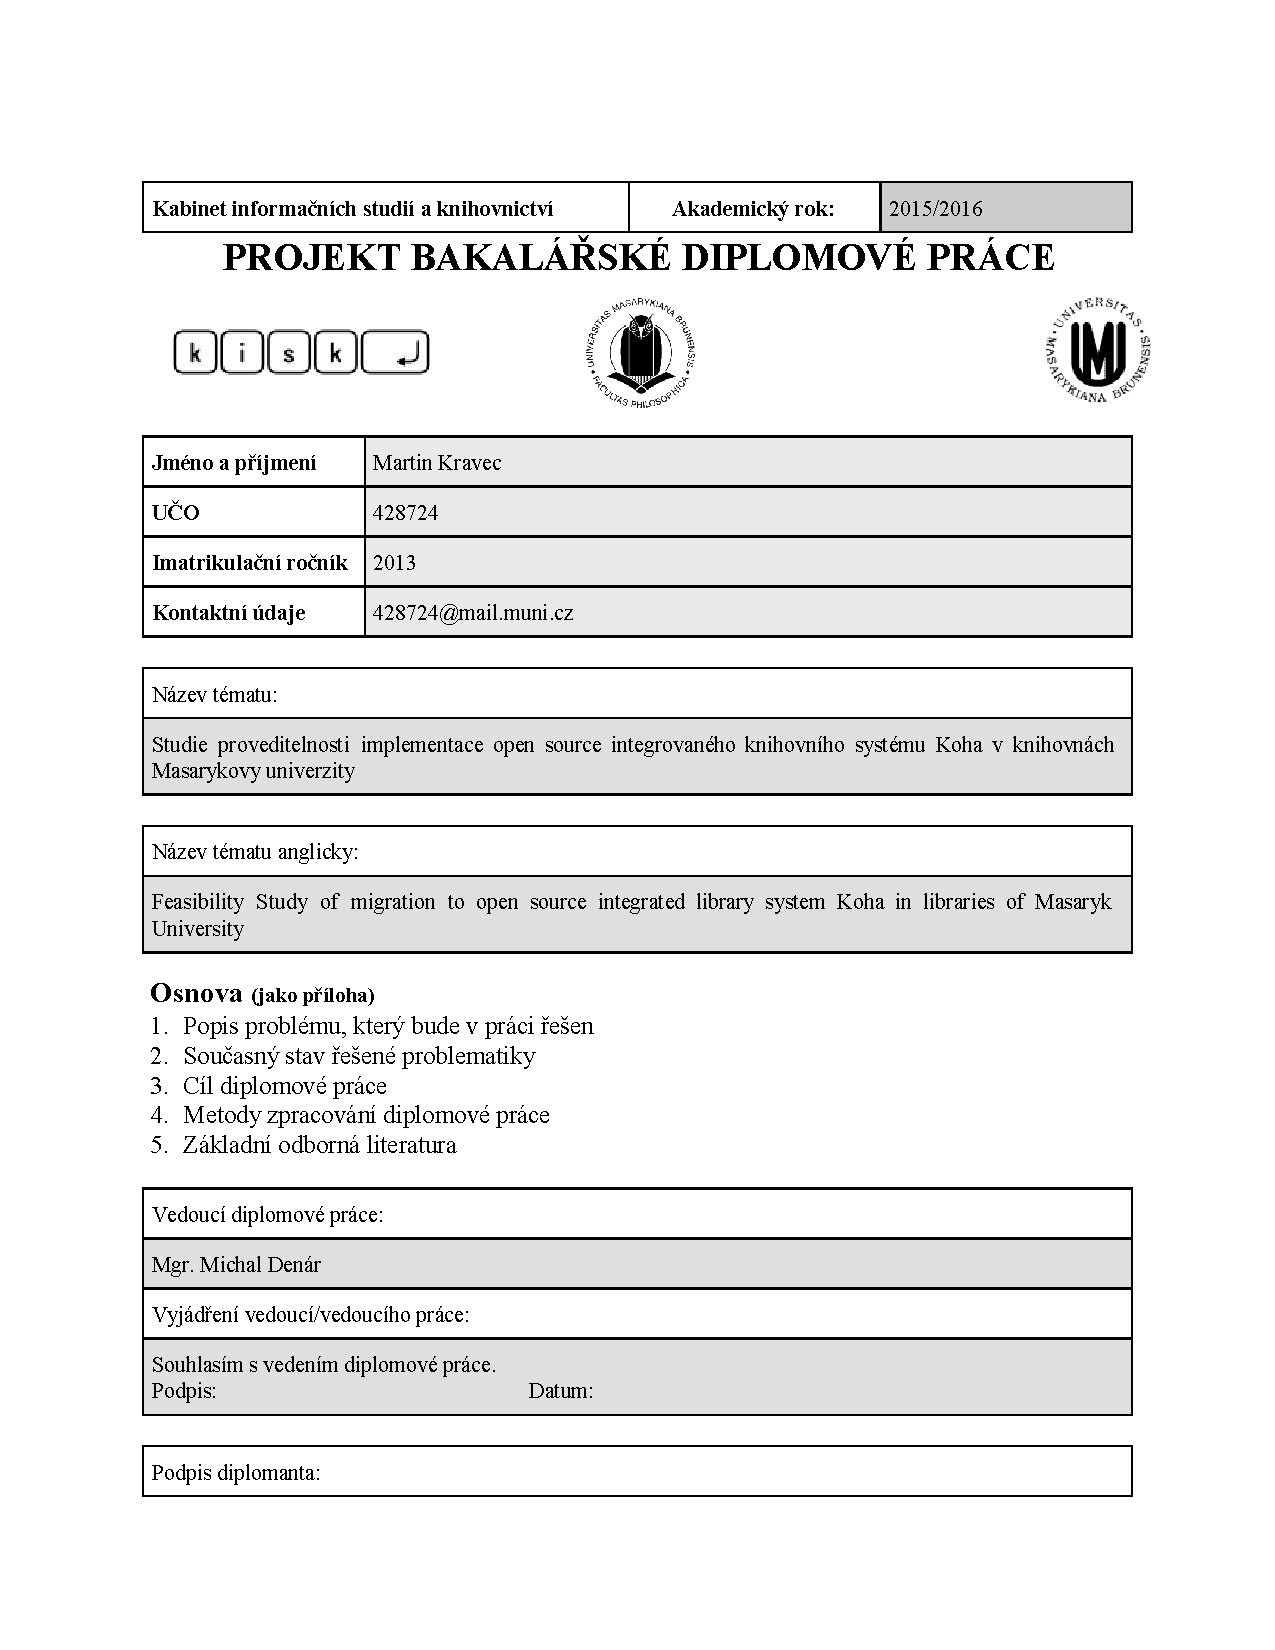
\includepdf[scale=1.05,pages={-}]{projekt.pdf}
  }
\makeatother

%%%%%%%%%%%%%%%%%%%%% DOCUMENT STRUCTURE %%%%%%%%%%%%%%%%%%%%

\makeatletter
  \def\thesis@blocks@preamble{
    \thesis@blocks@preTitlePage
    \thesis@blocks@coverMatter
    \thesis@blocks@cover
    \thesis@blocks@titlePage
    \thesis@blocks@frontMatter
      \noindent{\Large{Bibliografický záznam}}\newline\newline
        KRAVEC, Martin. \italic{\thesis@title}. Brno: Masarykova univerzita, Filozofická fakulta, 2016. 57 s. Vedoucí diplomové práce Mgr. Michal Denár.
	  \newline\newline
      {\Large{Anotace}}\newline\newline
        \thesis@abstract\newline\newline
      {\Large{Annotation}}\newline\newline
        \thesis@abstractEn\newline\newline
      \\%
      {\Large{Klíčová slova}}\newline\newline
        \thesis@keywords\newline\newline
      {\Large{Keywords}}\newline\newline
        \thesis@TeXkeywordsEn\newline\newline
  \thesis@blocks@declaration
  \thesis@blocks@thanks
  \thesis@blocks@clear
	\tableofcontents}
  \def\thesis@blocks@postamble{
    \addcontentsline{toc}{chapter}{\listtablename}
    \thesis@blocks@lot
    \addcontentsline{toc}{chapter}{\listfigurename}
    \thesis@blocks@lof
    \thesis@blocks@seznampriloh
    \thesis@blocks@prilohy}
\makeatother
  
%%%%%%%%%%%%%%%%%%%%%%%%%%%%% DOCUMENT %%%%%%%%%%%%%%%%%%%%%%%%%%%%%
\begin{document}{%\fontsize{11}{24}

\chapter*{Úvod}
\addcontentsline{toc}{chapter}{Úvod} 
Tato bakalářská diplomová práce se bude zabývat studií proveditelnosti implementace open source integrovaného knihovního systému Koha v~knihovnách Masarykovy univerzity. V~práci bude probíráno několik úhlů pohledu na celkovou problematiku, a~to v~kontextu studie proveditelnosti.  V~práci tedy rozebereme nejdřív teoretickou část knihovních systémů, co by měly umět a~jaký je jejich cíl jako produktu softwarových firem, to znamená, že probereme technické zastřešení projektu a~vysvětlíme veškeré pojmy s~tím spojené. Teoretická část dále vysvětlí oblast projektového managmentu a~přiblíží problematiku migrací na nový knihovní systém. Celý projekt bude řešen jako harmonogram realizace spolu s~finanční a~ekonomickou analýzou. V~rámci studie byl prováděn několikaměsíční průzkum v~knihovnách Masarykovy univerzity a~průzkum v~síti 900 knihoven v~Turecku. Při průzkumu byla realizována také SWOT analýza, na které je pak založeno celé hodnocení efektivity a~udržitelnosti projektu, ve kterém nebude chybět analýza a~řízení případných rizik, které s~sebou projekt migrace nese.

\chapter{Teoretická část}

\section{Projektové řízení jako takové} \label{sec:projektove_rizeni_jako_takove}

\subsection{Projekt}

Projektové řízení neboli projektový management se zabývá řízením projektů. Jeho cíle lze rozdělit na 3 části: 
\mezera
\begin{itemize}
\item splnění požadavků
\item časový plán
\item rozpočtové náklady
\end{itemize}

Tomuto rozdělení se také říká trojimperativ \citepages{5}{rosenau_2000}. O~každém projektu lze prohlásit, že je jedinečný, jelikož je prováděn jen jednou, pracují na něm jiní lidé a~je časově ohraničen. Projekt je realizován pomocí lidských a~materiálních zdrojů. To znamená, že projektový manager vlastně řídí lidi tak, aby byly efektivně využity materiální zdroje \citepages{28}{rehacek_2013}. Následující obrázek \ref{fig:trojimperativ} znázorňuje kvalitu provedení v~kontextu trojimperativu.

\begin{figure}
    \centering
	\def\svgwidth{1.0\textwidth}
    %LaTeX with PSTricks extensions
%%Creator: inkscape 0.48.4
%%Please note this file requires PSTricks extensions
\psset{xunit=.5pt,yunit=.5pt,runit=.5pt}
\begin{pspicture}(1152,864)
{
\newrgbcolor{curcolor}{0 0 0}
\pscustom[linestyle=none,fillstyle=solid,fillcolor=curcolor,opacity=0]
{
\newpath
\moveto(0,864)
\lineto(1152,864)
\lineto(1152,0)
\lineto(0,0)
\closepath
}
}
{
\newrgbcolor{curcolor}{0 0 0}
\pscustom[linestyle=none,fillstyle=solid,fillcolor=curcolor,opacity=0]
{
\newpath
\moveto(337.39108,587.4987)
\curveto(349.905515,551.456708)(343.564725,415.79835)(412.47769,371.24672)
\curveto(481.39062,326.695145)(694.47027,328.698624)(750.86877,320.18898)
}
}
{
\newrgbcolor{curcolor}{0 0 0}
\pscustom[linewidth=1,linecolor=curcolor]
{
\newpath
\moveto(337.39108,587.4987)
\curveto(349.905515,551.456708)(343.564725,415.79835)(412.47769,371.24672)
\curveto(481.39062,326.695145)(694.47027,328.698624)(750.86877,320.18898)
}
}
{
\newrgbcolor{curcolor}{0 0 0}
\pscustom[linestyle=none,fillstyle=solid,fillcolor=curcolor,opacity=0]
{
\newpath
\moveto(414.48032,370.2467)
\lineto(274.32285,370.2467)
}
}
{
\newrgbcolor{curcolor}{0 0 0}
\pscustom[linewidth=1,linecolor=curcolor,linestyle=dashed,dash=1 3]
{
\newpath
\moveto(414.48032,370.2467)
\lineto(274.32285,370.2467)
}
}
{
\newrgbcolor{curcolor}{0 0 0}
\pscustom[linestyle=none,fillstyle=solid,fillcolor=curcolor,opacity=0]
{
\newpath
\moveto(414.48032,370.2467)
\lineto(414.48032,270.12072)
}
}
{
\newrgbcolor{curcolor}{0 0 0}
\pscustom[linewidth=1,linecolor=curcolor,linestyle=dashed,dash=1 3]
{
\newpath
\moveto(414.48032,370.2467)
\lineto(414.48032,270.12072)
}
}
{
\newrgbcolor{curcolor}{0 0 0}
\pscustom[linestyle=none,fillstyle=solid,fillcolor=curcolor,opacity=0]
{
\newpath
\moveto(194.2441,597.52493)
\lineto(289.36222,597.52493)
\lineto(289.36222,562.469815)
\lineto(194.2441,562.469815)
\closepath
}
}
{
\newrgbcolor{curcolor}{0 0 0}
\pscustom[linestyle=none,fillstyle=solid,fillcolor=curcolor]
{
\newpath
\moveto(204.8066,570.60495)
\lineto(204.8066,584.1987)
\lineto(213.978475,584.1987)
\lineto(213.978475,582.60495)
\lineto(206.603475,582.60495)
\lineto(206.603475,578.3862)
\lineto(212.978475,578.3862)
\lineto(212.978475,576.776825)
\lineto(206.603475,576.776825)
\lineto(206.603475,570.60495)
\lineto(204.8066,570.60495)
\closepath
\moveto(215.905706,582.29245)
\lineto(215.905706,584.1987)
\lineto(217.577581,584.1987)
\lineto(217.577581,582.29245)
\lineto(215.905706,582.29245)
\closepath
\moveto(215.905706,570.60495)
\lineto(215.905706,580.464325)
\lineto(217.577581,580.464325)
\lineto(217.577581,570.60495)
\lineto(215.905706,570.60495)
\closepath
\moveto(220.034902,570.60495)
\lineto(220.034902,580.464325)
\lineto(221.534902,580.464325)
\lineto(221.534902,579.058075)
\curveto(222.26406867,580.14140833)(223.31094367,580.683075)(224.675527,580.683075)
\curveto(225.269277,580.683075)(225.816152,580.5737)(226.316152,580.35495)
\curveto(226.816152,580.14661667)(227.18594367,579.86536667)(227.425527,579.5112)
\curveto(227.675527,579.16745)(227.85261033,578.7612)(227.956777,578.29245)
\curveto(228.019277,577.97995)(228.050527,577.43828333)(228.050527,576.66745)
\lineto(228.050527,570.60495)
\lineto(226.378652,570.60495)
\lineto(226.378652,576.60495)
\curveto(226.378652,577.28203333)(226.31094367,577.78724167)(226.175527,578.120575)
\curveto(226.050527,578.464325)(225.82136033,578.73515833)(225.488027,578.933075)
\curveto(225.15469367,579.13099167)(224.76406867,579.22995)(224.316152,579.22995)
\curveto(223.60781867,579.22995)(222.99323533,579.00599167)(222.472402,578.558075)
\curveto(221.96198533,578.11015833)(221.706777,577.25078333)(221.706777,575.97995)
\lineto(221.706777,570.60495)
\lineto(220.034902,570.60495)
\closepath
\moveto(236.848119,571.8237)
\curveto(236.223119,571.29245)(235.62416067,570.91745)(235.051244,570.6987)
\curveto(234.47832733,570.49036667)(233.863744,570.3862)(233.207494,570.3862)
\curveto(232.13457733,570.3862)(231.30645233,570.64661667)(230.723119,571.16745)
\curveto(230.13978567,571.6987)(229.848119,572.37578333)(229.848119,573.1987)
\curveto(229.848119,573.68828333)(229.957494,574.13099167)(230.176244,574.526825)
\curveto(230.394994,574.92265833)(230.68145233,575.24036667)(231.035619,575.47995)
\curveto(231.38978567,575.71953333)(231.79082733,575.901825)(232.238744,576.026825)
\curveto(232.57207733,576.120575)(233.066869,576.20390833)(233.723119,576.276825)
\curveto(235.07728567,576.44349167)(236.07207733,576.6362)(236.707494,576.85495)
\lineto(236.707494,577.29245)
\curveto(236.707494,577.96953333)(236.551244,578.4487)(236.238744,578.72995)
\curveto(235.81166067,579.10495)(235.176244,579.29245)(234.332494,579.29245)
\curveto(233.551244,579.29245)(232.973119,579.15703333)(232.598119,578.8862)
\curveto(232.223119,578.61536667)(231.94707733,578.12578333)(231.769994,577.41745)
\lineto(230.129369,577.651825)
\curveto(230.285619,578.34974167)(230.53041067,578.91224167)(230.863744,579.339325)
\curveto(231.207494,579.76640833)(231.69707733,580.09453333)(232.332494,580.3237)
\curveto(232.97832733,580.56328333)(233.72832733,580.683075)(234.582494,580.683075)
\curveto(235.426244,580.683075)(236.10853567,580.58411667)(236.629369,580.3862)
\curveto(237.15020233,580.18828333)(237.535619,579.93828333)(237.785619,579.6362)
\curveto(238.035619,579.33411667)(238.207494,578.95390833)(238.301244,578.495575)
\curveto(238.363744,578.214325)(238.394994,577.70390833)(238.394994,576.964325)
\lineto(238.394994,574.72995)
\curveto(238.394994,573.17786667)(238.426244,572.19349167)(238.488744,571.776825)
\curveto(238.56166067,571.370575)(238.707494,570.97995)(238.926244,570.60495)
\lineto(237.176244,570.60495)
\curveto(236.99916067,570.9487)(236.88978567,571.35495)(236.848119,571.8237)
\closepath
\moveto(236.707494,575.54245)
\curveto(236.10332733,575.30286667)(235.191869,575.09453333)(233.973119,574.91745)
\curveto(233.285619,574.8237)(232.801244,574.714325)(232.519994,574.589325)
\curveto(232.238744,574.464325)(232.019994,574.28203333)(231.863744,574.04245)
\curveto(231.707494,573.80286667)(231.629369,573.53724167)(231.629369,573.245575)
\curveto(231.629369,572.79765833)(231.79603567,572.42265833)(232.129369,572.120575)
\curveto(232.473119,571.82890833)(232.96791067,571.683075)(233.613744,571.683075)
\curveto(234.25957733,571.683075)(234.832494,571.8237)(235.332494,572.10495)
\curveto(235.832494,572.39661667)(236.20228567,572.78203333)(236.441869,573.2612)
\curveto(236.61895233,573.64661667)(236.707494,574.20390833)(236.707494,574.933075)
\lineto(236.707494,575.54245)
\closepath
\moveto(240.786336,570.60495)
\lineto(240.786336,580.464325)
\lineto(242.286336,580.464325)
\lineto(242.286336,579.058075)
\curveto(243.01550267,580.14140833)(244.06237767,580.683075)(245.426961,580.683075)
\curveto(246.020711,580.683075)(246.567586,580.5737)(247.067586,580.35495)
\curveto(247.567586,580.14661667)(247.93737767,579.86536667)(248.176961,579.5112)
\curveto(248.426961,579.16745)(248.60404433,578.7612)(248.708211,578.29245)
\curveto(248.770711,577.97995)(248.801961,577.43828333)(248.801961,576.66745)
\lineto(248.801961,570.60495)
\lineto(247.130086,570.60495)
\lineto(247.130086,576.60495)
\curveto(247.130086,577.28203333)(247.06237767,577.78724167)(246.926961,578.120575)
\curveto(246.801961,578.464325)(246.57279433,578.73515833)(246.239461,578.933075)
\curveto(245.90612767,579.13099167)(245.51550267,579.22995)(245.067586,579.22995)
\curveto(244.35925267,579.22995)(243.74466933,579.00599167)(243.223836,578.558075)
\curveto(242.71341933,578.11015833)(242.458211,577.25078333)(242.458211,575.97995)
\lineto(242.458211,570.60495)
\lineto(240.786336,570.60495)
\closepath
\moveto(257.599553,574.214325)
\lineto(259.240178,573.995575)
\curveto(259.06309467,572.870575)(258.60476133,571.98515833)(257.865178,571.339325)
\curveto(257.12559467,570.70390833)(256.21413633,570.3862)(255.130803,570.3862)
\curveto(253.787053,570.3862)(252.70371967,570.8237)(251.880803,571.6987)
\curveto(251.068303,572.58411667)(250.662053,573.84974167)(250.662053,575.495575)
\curveto(250.662053,576.558075)(250.833928,577.48515833)(251.177678,578.276825)
\curveto(251.53184467,579.07890833)(252.068303,579.67786667)(252.787053,580.0737)
\curveto(253.51621967,580.47995)(254.302678,580.683075)(255.146428,580.683075)
\curveto(256.21934467,580.683075)(257.09434467,580.41224167)(257.771428,579.870575)
\curveto(258.44851133,579.32890833)(258.88601133,578.558075)(259.083928,577.558075)
\lineto(257.458928,577.308075)
\curveto(257.302678,577.97474167)(257.02663633,578.47474167)(256.630803,578.808075)
\curveto(256.23496967,579.14140833)(255.76101133,579.308075)(255.208928,579.308075)
\curveto(254.365178,579.308075)(253.677678,579.00599167)(253.146428,578.401825)
\curveto(252.62559467,577.79765833)(252.365178,576.84453333)(252.365178,575.54245)
\curveto(252.365178,574.21953333)(252.62038633,573.25599167)(253.130803,572.651825)
\curveto(253.64121967,572.058075)(254.302678,571.7612)(255.115178,571.7612)
\curveto(255.771428,571.7612)(256.318303,571.95911667)(256.755803,572.35495)
\curveto(257.193303,572.7612)(257.474553,573.38099167)(257.599553,574.214325)
\closepath
\moveto(267.240178,573.776825)
\lineto(268.958928,573.558075)
\curveto(268.68809467,572.558075)(268.18288633,571.776825)(267.443303,571.214325)
\curveto(266.71413633,570.66224167)(265.77663633,570.3862)(264.630803,570.3862)
\curveto(263.193303,570.3862)(262.052678,570.82890833)(261.208928,571.714325)
\curveto(260.365178,572.59974167)(259.943303,573.84453333)(259.943303,575.4487)
\curveto(259.943303,577.10495)(260.365178,578.39140833)(261.208928,579.308075)
\curveto(262.06309467,580.22474167)(263.17246967,580.683075)(264.537053,580.683075)
\curveto(265.85996967,580.683075)(266.93809467,580.23515833)(267.771428,579.339325)
\curveto(268.60476133,578.44349167)(269.021428,577.17786667)(269.021428,575.54245)
\curveto(269.021428,575.4487)(269.01621967,575.30286667)(269.005803,575.10495)
\lineto(261.662053,575.10495)
\curveto(261.724553,574.02161667)(262.03184467,573.19349167)(262.583928,572.620575)
\curveto(263.13601133,572.04765833)(263.82351133,571.7612)(264.646428,571.7612)
\curveto(265.25059467,571.7612)(265.76621967,571.91745)(266.193303,572.22995)
\curveto(266.630803,572.55286667)(266.97976133,573.06849167)(267.240178,573.776825)
\closepath
\moveto(261.755803,576.47995)
\lineto(267.255803,576.47995)
\curveto(267.18288633,577.30286667)(266.974553,577.92265833)(266.630803,578.339325)
\curveto(266.099553,578.98515833)(265.40684467,579.308075)(264.552678,579.308075)
\curveto(263.79226133,579.308075)(263.146428,579.04765833)(262.615178,578.526825)
\curveto(262.09434467,578.01640833)(261.80788633,577.33411667)(261.755803,576.47995)
\closepath
}
}
{
\newrgbcolor{curcolor}{0 0 0}
\pscustom[linestyle=none,fillstyle=solid,fillcolor=curcolor,opacity=0]
{
\newpath
\moveto(192.2231,391.27036)
\lineto(295.34122,391.27036)
\lineto(295.34122,349.22309)
\lineto(192.2231,349.22309)
\closepath
}
}
{
\newrgbcolor{curcolor}{0 0 0}
\pscustom[linestyle=none,fillstyle=solid,fillcolor=curcolor]
{
\newpath
\moveto(202.48872,366.91034)
\lineto(202.48872,378.363465)
\lineto(207.566845,378.363465)
\curveto(208.58767833,378.363465)(209.36372,378.25929833)(209.89497,378.050965)
\curveto(210.42622,377.85304833)(210.848095,377.49367333)(211.160595,376.97284)
\curveto(211.48351167,376.45200667)(211.64497,375.87388167)(211.64497,375.238465)
\curveto(211.64497,374.425965)(211.379345,373.738465)(210.848095,373.175965)
\curveto(210.32726167,372.62388167)(209.51476167,372.27492333)(208.410595,372.12909)
\curveto(208.816845,371.93117333)(209.12413667,371.738465)(209.33247,371.550965)
\curveto(209.76997,371.144715)(210.18663667,370.63950667)(210.58247,370.03534)
\lineto(212.58247,366.91034)
\lineto(210.67622,366.91034)
\lineto(209.160595,369.300965)
\curveto(208.71267833,369.988465)(208.34288667,370.51450667)(208.05122,370.87909)
\curveto(207.76997,371.24367333)(207.51476167,371.49888167)(207.285595,371.644715)
\curveto(207.066845,371.79054833)(206.83767833,371.88950667)(206.598095,371.94159)
\curveto(206.43142833,371.98325667)(206.15017833,372.00409)(205.754345,372.00409)
\lineto(204.004345,372.00409)
\lineto(204.004345,366.91034)
\lineto(202.48872,366.91034)
\closepath
\moveto(204.004345,373.31659)
\lineto(207.254345,373.31659)
\curveto(207.95226167,373.31659)(208.49392833,373.38429833)(208.879345,373.519715)
\curveto(209.27517833,373.66554833)(209.57205333,373.894715)(209.76997,374.207215)
\curveto(209.97830333,374.53013167)(210.08247,374.87388167)(210.08247,375.238465)
\curveto(210.08247,375.78013167)(209.88455333,376.22284)(209.48872,376.56659)
\curveto(209.09288667,376.92075667)(208.473095,377.09784)(207.629345,377.09784)
\lineto(204.004345,377.09784)
\lineto(204.004345,373.31659)
\closepath
\moveto(213.3090325,371.06659)
\curveto(213.3090325,372.59784)(213.73611583,373.73325667)(214.5902825,374.47284)
\curveto(215.3090325,375.08742333)(216.17882417,375.394715)(217.1996575,375.394715)
\curveto(218.34549083,375.394715)(219.2777825,375.019715)(219.9965325,374.269715)
\curveto(220.72569917,373.53013167)(221.0902825,372.49888167)(221.0902825,371.175965)
\curveto(221.0902825,370.113465)(220.92882417,369.27492333)(220.6059075,368.66034)
\curveto(220.28299083,368.04575667)(219.81424083,367.56659)(219.1996575,367.22284)
\curveto(218.59549083,366.88950667)(217.92882417,366.72284)(217.1996575,366.72284)
\curveto(216.0434075,366.72284)(215.1059075,367.09263167)(214.3871575,367.832215)
\curveto(213.6684075,368.582215)(213.3090325,369.66034)(213.3090325,371.06659)
\closepath
\moveto(214.7621575,371.06659)
\curveto(214.7621575,370.00409)(214.99132417,369.207215)(215.4496575,368.675965)
\curveto(215.9184075,368.144715)(216.50174083,367.87909)(217.1996575,367.87909)
\curveto(217.89757417,367.87909)(218.47569917,368.144715)(218.9340325,368.675965)
\curveto(219.4027825,369.207215)(219.6371575,370.019715)(219.6371575,371.113465)
\curveto(219.6371575,372.13429833)(219.4027825,372.91034)(218.9340325,373.44159)
\curveto(218.47569917,373.97284)(217.89757417,374.238465)(217.1996575,374.238465)
\curveto(216.50174083,374.238465)(215.9184075,373.97284)(215.4496575,373.44159)
\curveto(214.99132417,372.92075667)(214.7621575,372.12909)(214.7621575,371.06659)
\closepath
\moveto(221.98872,366.91034)
\lineto(221.98872,368.050965)
\lineto(227.26997,374.113465)
\curveto(226.67622,374.082215)(226.15017833,374.06659)(225.691845,374.06659)
\lineto(222.30122,374.06659)
\lineto(222.30122,375.207215)
\lineto(229.08247,375.207215)
\lineto(229.08247,374.28534)
\lineto(224.598095,369.019715)
\lineto(223.723095,368.050965)
\curveto(224.35851167,368.10304833)(224.95226167,368.12909)(225.504345,368.12909)
\lineto(229.33247,368.12909)
\lineto(229.33247,366.91034)
\lineto(221.98872,366.91034)
\closepath
\moveto(230.73872,363.72284)
\lineto(230.73872,375.207215)
\lineto(232.01997,375.207215)
\lineto(232.01997,374.12909)
\curveto(232.32205333,374.55617333)(232.660595,374.87388167)(233.035595,375.082215)
\curveto(233.42101167,375.29054833)(233.88455333,375.394715)(234.42622,375.394715)
\curveto(235.13455333,375.394715)(235.75955333,375.21242333)(236.30122,374.84784)
\curveto(236.84288667,374.48325667)(237.24913667,373.96763167)(237.51997,373.300965)
\curveto(237.80122,372.644715)(237.941845,371.92075667)(237.941845,371.12909)
\curveto(237.941845,370.27492333)(237.785595,369.50929833)(237.473095,368.832215)
\curveto(237.17101167,368.15513167)(236.72830333,367.63429833)(236.14497,367.269715)
\curveto(235.57205333,366.90513167)(234.96267833,366.72284)(234.316845,366.72284)
\curveto(233.848095,366.72284)(233.42622,366.82179833)(233.05122,367.019715)
\curveto(232.68663667,367.21763167)(232.38455333,367.46763167)(232.14497,367.769715)
\lineto(232.14497,363.72284)
\lineto(230.73872,363.72284)
\closepath
\moveto(232.004345,371.019715)
\curveto(232.004345,369.94679833)(232.21788667,369.15513167)(232.64497,368.644715)
\curveto(233.08247,368.13429833)(233.60851167,367.87909)(234.223095,367.87909)
\curveto(234.848095,367.87909)(235.38455333,368.144715)(235.83247,368.675965)
\curveto(236.28038667,369.207215)(236.504345,370.02492333)(236.504345,371.12909)
\curveto(236.504345,372.19159)(236.285595,372.98325667)(235.848095,373.50409)
\curveto(235.410595,374.03534)(234.88976167,374.300965)(234.285595,374.300965)
\curveto(233.691845,374.300965)(233.160595,374.019715)(232.691845,373.457215)
\curveto(232.23351167,372.894715)(232.004345,372.082215)(232.004345,371.019715)
\closepath
\moveto(239.1059075,371.06659)
\curveto(239.1059075,372.59784)(239.53299083,373.73325667)(240.3871575,374.47284)
\curveto(241.1059075,375.08742333)(241.97569917,375.394715)(242.9965325,375.394715)
\curveto(244.14236583,375.394715)(245.0746575,375.019715)(245.7934075,374.269715)
\curveto(246.52257417,373.53013167)(246.8871575,372.49888167)(246.8871575,371.175965)
\curveto(246.8871575,370.113465)(246.72569917,369.27492333)(246.4027825,368.66034)
\curveto(246.07986583,368.04575667)(245.61111583,367.56659)(244.9965325,367.22284)
\curveto(244.39236583,366.88950667)(243.72569917,366.72284)(242.9965325,366.72284)
\curveto(241.8402825,366.72284)(240.9027825,367.09263167)(240.1840325,367.832215)
\curveto(239.4652825,368.582215)(239.1059075,369.66034)(239.1059075,371.06659)
\closepath
\moveto(240.5590325,371.06659)
\curveto(240.5590325,370.00409)(240.78819917,369.207215)(241.2465325,368.675965)
\curveto(241.7152825,368.144715)(242.29861583,367.87909)(242.9965325,367.87909)
\curveto(243.69444917,367.87909)(244.27257417,368.144715)(244.7309075,368.675965)
\curveto(245.1996575,369.207215)(245.4340325,370.019715)(245.4340325,371.113465)
\curveto(245.4340325,372.13429833)(245.1996575,372.91034)(244.7309075,373.44159)
\curveto(244.27257417,373.97284)(243.69444917,374.238465)(242.9965325,374.238465)
\curveto(242.29861583,374.238465)(241.7152825,373.97284)(241.2465325,373.44159)
\curveto(240.78819917,372.92075667)(240.5590325,372.12909)(240.5590325,371.06659)
\closepath
\moveto(253.941845,369.957215)
\lineto(255.33247,369.769715)
\curveto(255.17622,368.82179833)(254.785595,368.07700667)(254.160595,367.53534)
\curveto(253.54601167,366.99367333)(252.785595,366.72284)(251.879345,366.72284)
\curveto(250.74392833,366.72284)(249.82726167,367.09263167)(249.129345,367.832215)
\curveto(248.441845,368.582215)(248.098095,369.64992333)(248.098095,371.03534)
\curveto(248.098095,371.93117333)(248.24392833,372.71242333)(248.535595,373.37909)
\curveto(248.83767833,374.05617333)(249.29080333,374.56138167)(249.89497,374.894715)
\curveto(250.50955333,375.22804833)(251.17101167,375.394715)(251.879345,375.394715)
\curveto(252.785595,375.394715)(253.52517833,375.16554833)(254.098095,374.707215)
\curveto(254.67101167,374.25929833)(255.035595,373.613465)(255.191845,372.769715)
\lineto(253.83247,372.56659)
\curveto(253.69705333,373.11867333)(253.46267833,373.53534)(253.129345,373.81659)
\curveto(252.80642833,374.09784)(252.410595,374.238465)(251.941845,374.238465)
\curveto(251.23351167,374.238465)(250.65538667,373.98325667)(250.20747,373.47284)
\curveto(249.76997,372.97284)(249.55122,372.17075667)(249.55122,371.06659)
\curveto(249.55122,369.95200667)(249.76476167,369.13950667)(250.191845,368.62909)
\curveto(250.61892833,368.12909)(251.17622,367.87909)(251.86372,367.87909)
\curveto(252.41580333,367.87909)(252.87413667,368.04575667)(253.23872,368.37909)
\curveto(253.61372,368.72284)(253.848095,369.24888167)(253.941845,369.957215)
\closepath
\moveto(252.285595,377.09784)
\lineto(253.14497,378.425965)
\lineto(254.73872,378.425965)
\lineto(252.973095,376.238465)
\lineto(251.473095,376.238465)
\lineto(249.785595,378.425965)
\lineto(251.39497,378.425965)
\lineto(252.285595,377.09784)
\closepath
\moveto(262.207455,369.582215)
\lineto(263.66058,369.41034)
\curveto(263.43141333,368.55617333)(263.00433,367.894715)(262.37933,367.425965)
\curveto(261.76474667,366.957215)(260.97828833,366.72284)(260.019955,366.72284)
\curveto(258.801205,366.72284)(257.83766333,367.09784)(257.12933,367.84784)
\curveto(256.42099667,368.59784)(256.06683,369.644715)(256.06683,370.988465)
\curveto(256.06683,372.38429833)(256.426205,373.46763167)(257.144955,374.238465)
\curveto(257.863705,375.00929833)(258.79599667,375.394715)(259.94183,375.394715)
\curveto(261.04599667,375.394715)(261.94703833,375.01450667)(262.644955,374.25409)
\curveto(263.35328833,373.50409)(263.707455,372.44679833)(263.707455,371.082215)
\lineto(263.707455,370.707215)
\lineto(257.519955,370.707215)
\curveto(257.57203833,369.79054833)(257.82724667,369.08742333)(258.28558,368.59784)
\curveto(258.75433,368.11867333)(259.332455,367.87909)(260.019955,367.87909)
\curveto(260.54078833,367.87909)(260.98349667,368.01450667)(261.34808,368.28534)
\curveto(261.71266333,368.55617333)(261.99912167,368.988465)(262.207455,369.582215)
\closepath
\moveto(257.59808,371.863465)
\lineto(262.22308,371.863465)
\curveto(262.16058,372.56138167)(261.98349667,373.082215)(261.69183,373.425965)
\curveto(261.24391333,373.96763167)(260.66578833,374.238465)(259.957455,374.238465)
\curveto(259.31162167,374.238465)(258.76474667,374.019715)(258.31683,373.582215)
\curveto(257.87933,373.15513167)(257.63974667,372.582215)(257.59808,371.863465)
\closepath
\moveto(268.4965175,368.175965)
\lineto(268.6996425,366.925965)
\curveto(268.30380917,366.84263167)(267.9496425,366.800965)(267.6371425,366.800965)
\curveto(267.12672583,366.800965)(266.7308925,366.87909)(266.4496425,367.03534)
\curveto(266.1683925,367.20200667)(265.97047583,367.41554833)(265.8558925,367.675965)
\curveto(265.74130917,367.94679833)(265.6840175,368.50409)(265.6840175,369.34784)
\lineto(265.6840175,374.113465)
\lineto(264.6527675,374.113465)
\lineto(264.6527675,375.207215)
\lineto(265.6840175,375.207215)
\lineto(265.6840175,377.269715)
\lineto(267.0902675,378.113465)
\lineto(267.0902675,375.207215)
\lineto(268.4965175,375.207215)
\lineto(268.4965175,374.113465)
\lineto(267.0902675,374.113465)
\lineto(267.0902675,369.269715)
\curveto(267.0902675,368.863465)(267.11110083,368.60304833)(267.1527675,368.488465)
\curveto(267.20485083,368.37388167)(267.28818417,368.28013167)(267.4027675,368.207215)
\curveto(267.51735083,368.144715)(267.67880917,368.113465)(267.8871425,368.113465)
\curveto(268.0433925,368.113465)(268.2465175,368.13429833)(268.4965175,368.175965)
\closepath
}
}
{
\newrgbcolor{curcolor}{0 0 0}
\pscustom[linestyle=none,fillstyle=solid,fillcolor=curcolor,opacity=0]
{
\newpath
\moveto(241.7769,385.2546)
\lineto(241.7769,550.45144)
\lineto(341.90289,550.45144)
\lineto(341.90289,385.2546)
\closepath
}
}
{
\newrgbcolor{curcolor}{0 0 0}
\pscustom[linestyle=none,fillstyle=solid,fillcolor=curcolor]
{
\newpath
\moveto(263.5769,395.2546)
\lineto(254.2644,395.2546)
\lineto(254.2644,398.770225)
\curveto(254.2644,399.38480833)(254.29565,399.85355833)(254.35815,400.176475)
\curveto(254.43106667,400.63480833)(254.5769,401.020225)(254.79565,401.332725)
\curveto(255.00398333,401.645225)(255.30085833,401.895225)(255.686275,402.082725)
\curveto(256.07169167,402.270225)(256.498775,402.363975)(256.967525,402.363975)
\curveto(257.75919167,402.363975)(258.43106667,402.10876667)(258.98315,401.59835)
\curveto(259.52481667,401.09835)(259.79565,400.1921)(259.79565,398.8796)
\lineto(259.79565,396.488975)
\lineto(263.5769,396.488975)
\lineto(263.5769,395.2546)
\closepath
\moveto(258.7019,396.488975)
\lineto(258.7019,398.895225)
\curveto(258.7019,399.68689167)(258.55606667,400.24939167)(258.2644,400.582725)
\curveto(257.96231667,400.926475)(257.54044167,401.09835)(256.998775,401.09835)
\curveto(256.61335833,401.09835)(256.28523333,400.99939167)(256.0144,400.801475)
\curveto(255.73315,400.60355833)(255.54565,400.34314167)(255.4519,400.020225)
\curveto(255.39981667,399.81189167)(255.373775,399.426475)(255.373775,398.863975)
\lineto(255.373775,396.488975)
\lineto(258.7019,396.488975)
\closepath
\moveto(263.5769,403.98809)
\lineto(256.842525,403.98809)
\lineto(256.842525,405.01934)
\lineto(257.85815,405.01934)
\curveto(257.37898333,405.27975667)(257.06648333,405.51934)(256.92065,405.73809)
\curveto(256.7644,405.96725667)(256.686275,406.21204833)(256.686275,406.472465)
\curveto(256.686275,406.85788167)(256.80606667,407.24850667)(257.04565,407.64434)
\lineto(258.10815,407.253715)
\curveto(257.94148333,406.972465)(257.85815,406.69642333)(257.85815,406.42559)
\curveto(257.85815,406.17559)(257.936275,405.94642333)(258.092525,405.73809)
\curveto(258.23835833,405.54017333)(258.44669167,405.39954833)(258.717525,405.316215)
\curveto(259.123775,405.191215)(259.56648333,405.128715)(260.04565,405.128715)
\lineto(263.5769,405.128715)
\lineto(263.5769,403.98809)
\closepath
\moveto(255.29565,405.42559)
\lineto(254.217525,406.128715)
\lineto(254.217525,407.409965)
\lineto(255.998775,405.98809)
\lineto(255.998775,404.76934)
\lineto(254.217525,403.39434)
\lineto(254.217525,404.70684)
\lineto(255.29565,405.42559)
\closepath
\moveto(261.405025,413.051475)
\lineto(261.54565,414.238975)
\curveto(262.24356667,414.051475)(262.78523333,413.70251667)(263.17065,413.1921)
\curveto(263.54565,412.6921)(263.73315,412.051475)(263.73315,411.270225)
\curveto(263.73315,410.28064167)(263.43106667,409.49418333)(262.8269,408.91085)
\curveto(262.21231667,408.33793333)(261.35815,408.051475)(260.2644,408.051475)
\curveto(259.12898333,408.051475)(258.248775,408.34314167)(257.623775,408.926475)
\curveto(256.998775,409.520225)(256.686275,410.28064167)(256.686275,411.207725)
\curveto(256.686275,412.113975)(256.99356667,412.84835)(257.60815,413.41085)
\curveto(258.22273333,413.98376667)(259.08210833,414.270225)(260.186275,414.270225)
\lineto(260.498775,414.270225)
\lineto(260.498775,409.238975)
\curveto(261.23835833,409.28064167)(261.80606667,409.488975)(262.2019,409.863975)
\curveto(262.59773333,410.238975)(262.79565,410.707725)(262.79565,411.270225)
\curveto(262.79565,411.69730833)(262.686275,412.05668333)(262.467525,412.34835)
\curveto(262.23835833,412.65043333)(261.88419167,412.88480833)(261.405025,413.051475)
\closepath
\moveto(259.561275,409.301475)
\lineto(259.561275,413.0671)
\curveto(258.98835833,413.01501667)(258.561275,412.86918333)(258.280025,412.6296)
\curveto(257.842525,412.26501667)(257.623775,411.79626667)(257.623775,411.22335)
\curveto(257.623775,410.6921)(257.80085833,410.24939167)(258.155025,409.895225)
\curveto(258.498775,409.54105833)(258.967525,409.34314167)(259.561275,409.301475)
\closepath
\moveto(261.10815,420.245201)
\lineto(261.248775,421.370201)
\curveto(262.030025,421.25561767)(262.6394,420.94311767)(263.0769,420.432701)
\curveto(263.5144,419.92228433)(263.73315,419.30249267)(263.73315,418.573326)
\curveto(263.73315,417.64624267)(263.43106667,416.901451)(262.8269,416.338951)
\curveto(262.22273333,415.78686767)(261.35815,415.510826)(260.23315,415.510826)
\curveto(259.50398333,415.510826)(258.86856667,415.63061767)(258.3269,415.870201)
\curveto(257.77481667,416.10978433)(257.36335833,416.47436767)(257.092525,416.963951)
\curveto(256.82169167,417.45353433)(256.686275,417.98999267)(256.686275,418.573326)
\curveto(256.686275,419.30249267)(256.873775,419.901451)(257.248775,420.370201)
\curveto(257.61335833,420.838951)(258.13419167,421.135826)(258.811275,421.260826)
\lineto(258.98315,420.151451)
\curveto(258.53523333,420.04728433)(258.19669167,419.85978433)(257.967525,419.588951)
\curveto(257.73835833,419.32853433)(257.623775,419.00561767)(257.623775,418.620201)
\curveto(257.623775,418.04728433)(257.83210833,417.57853433)(258.248775,417.213951)
\curveto(258.655025,416.85978433)(259.30606667,416.682701)(260.2019,416.682701)
\curveto(261.10815,416.682701)(261.76960833,416.854576)(262.186275,417.198326)
\curveto(262.592525,417.542076)(262.79565,417.995201)(262.79565,418.557701)
\curveto(262.79565,419.00561767)(262.66023333,419.38061767)(262.3894,419.682701)
\curveto(262.10815,419.98478433)(261.68106667,420.17228433)(261.10815,420.245201)
\closepath
\moveto(255.29565,418.276451)
\lineto(254.217525,418.979576)
\lineto(254.217525,420.260826)
\lineto(255.998775,418.838951)
\lineto(255.998775,417.620201)
\lineto(254.217525,416.245201)
\lineto(254.217525,417.557701)
\lineto(255.29565,418.276451)
\closepath
\moveto(261.405025,427.1280135)
\lineto(261.54565,428.3155135)
\curveto(262.24356667,428.1280135)(262.78523333,427.77905517)(263.17065,427.2686385)
\curveto(263.54565,426.7686385)(263.73315,426.1280135)(263.73315,425.3467635)
\curveto(263.73315,424.35718017)(263.43106667,423.57072183)(262.8269,422.9873885)
\curveto(262.21231667,422.41447183)(261.35815,422.1280135)(260.2644,422.1280135)
\curveto(259.12898333,422.1280135)(258.248775,422.41968017)(257.623775,423.0030135)
\curveto(256.998775,423.5967635)(256.686275,424.35718017)(256.686275,425.2842635)
\curveto(256.686275,426.1905135)(256.99356667,426.9248885)(257.60815,427.4873885)
\curveto(258.22273333,428.06030517)(259.08210833,428.3467635)(260.186275,428.3467635)
\lineto(260.498775,428.3467635)
\lineto(260.498775,423.3155135)
\curveto(261.23835833,423.35718017)(261.80606667,423.5655135)(262.2019,423.9405135)
\curveto(262.59773333,424.3155135)(262.79565,424.7842635)(262.79565,425.3467635)
\curveto(262.79565,425.77384683)(262.686275,426.13322183)(262.467525,426.4248885)
\curveto(262.23835833,426.72697183)(261.88419167,426.96134683)(261.405025,427.1280135)
\closepath
\moveto(259.561275,423.3780135)
\lineto(259.561275,427.1436385)
\curveto(258.98835833,427.09155517)(258.561275,426.94572183)(258.280025,426.7061385)
\curveto(257.842525,426.34155517)(257.623775,425.87280517)(257.623775,425.2998885)
\curveto(257.623775,424.7686385)(257.80085833,424.32593017)(258.155025,423.9717635)
\curveto(258.498775,423.61759683)(258.967525,423.41968017)(259.561275,423.3780135)
\closepath
\moveto(263.5769,429.9154891)
\lineto(256.842525,429.9154891)
\lineto(256.842525,430.9467391)
\lineto(257.85815,430.9467391)
\curveto(257.37898333,431.20715577)(257.06648333,431.4467391)(256.92065,431.6654891)
\curveto(256.7644,431.89465577)(256.686275,432.13944743)(256.686275,432.3998641)
\curveto(256.686275,432.78528077)(256.80606667,433.17590577)(257.04565,433.5717391)
\lineto(258.10815,433.1811141)
\curveto(257.94148333,432.8998641)(257.85815,432.62382243)(257.85815,432.3529891)
\curveto(257.85815,432.1029891)(257.936275,431.87382243)(258.092525,431.6654891)
\curveto(258.23835833,431.46757243)(258.44669167,431.32694743)(258.717525,431.2436141)
\curveto(259.123775,431.1186141)(259.56648333,431.0561141)(260.04565,431.0561141)
\lineto(263.5769,431.0561141)
\lineto(263.5769,429.9154891)
\closepath
\moveto(266.155025,434.3694686)
\lineto(256.842525,434.3694686)
\lineto(256.842525,435.4007186)
\lineto(257.717525,435.4007186)
\curveto(257.373775,435.6507186)(257.11856667,435.92676027)(256.9519,436.2288436)
\curveto(256.77481667,436.5413436)(256.686275,436.92155193)(256.686275,437.3694686)
\curveto(256.686275,437.94238527)(256.83731667,438.4475936)(257.1394,438.8850936)
\curveto(257.43106667,439.3225936)(257.84773333,439.6507186)(258.3894,439.8694686)
\curveto(258.92065,440.09863527)(259.50919167,440.2132186)(260.155025,440.2132186)
\curveto(260.842525,440.2132186)(261.46231667,440.0882186)(262.0144,439.8382186)
\curveto(262.56648333,439.59863527)(262.99356667,439.23926027)(263.29565,438.7600936)
\curveto(263.58731667,438.2913436)(263.73315,437.79655193)(263.73315,437.2757186)
\curveto(263.73315,436.9007186)(263.655025,436.56217693)(263.498775,436.2600936)
\curveto(263.33210833,435.95801027)(263.123775,435.70801027)(262.873775,435.5100936)
\lineto(266.155025,435.5100936)
\lineto(266.155025,434.3694686)
\closepath
\moveto(260.248775,435.4007186)
\curveto(261.11335833,435.4007186)(261.75398333,435.57780193)(262.17065,435.9319686)
\curveto(262.58731667,436.28613527)(262.79565,436.70801027)(262.79565,437.1975936)
\curveto(262.79565,437.70801027)(262.58210833,438.14551027)(262.155025,438.5100936)
\curveto(261.717525,438.87467693)(261.05085833,439.0569686)(260.155025,439.0569686)
\curveto(259.29044167,439.0569686)(258.64460833,438.87988527)(258.217525,438.5257186)
\curveto(257.79044167,438.17155193)(257.5769,437.74967693)(257.5769,437.2600936)
\curveto(257.5769,436.77051027)(257.80606667,436.3382186)(258.2644,435.9632186)
\curveto(258.71231667,435.5882186)(259.373775,435.4007186)(260.248775,435.4007186)
\closepath
\moveto(262.748775,446.1725696)
\curveto(263.10294167,445.75590293)(263.35815,445.34965293)(263.5144,444.9538196)
\curveto(263.66023333,444.56840293)(263.73315,444.15173627)(263.73315,443.7038196)
\curveto(263.73315,442.9538196)(263.55085833,442.38090293)(263.186275,441.9850696)
\curveto(262.82169167,441.58923627)(262.35815,441.3913196)(261.79565,441.3913196)
\curveto(261.47273333,441.3913196)(261.17585833,441.46423627)(260.905025,441.6100696)
\curveto(260.623775,441.7663196)(260.39981667,441.96423627)(260.23315,442.2038196)
\curveto(260.06648333,442.4538196)(259.94148333,442.72986127)(259.85815,443.0319446)
\curveto(259.80606667,443.2506946)(259.748775,443.58923627)(259.686275,444.0475696)
\curveto(259.58210833,444.96423627)(259.4519,445.6413196)(259.29565,446.0788196)
\curveto(259.1394,446.08923627)(259.04044167,446.0944446)(258.998775,446.0944446)
\curveto(258.530025,446.0944446)(258.2019,445.9850696)(258.0144,445.7663196)
\curveto(257.75398333,445.47465293)(257.623775,445.04236127)(257.623775,444.4694446)
\curveto(257.623775,443.92777793)(257.717525,443.52673627)(257.905025,443.2663196)
\curveto(258.092525,443.0163196)(258.42585833,442.8288196)(258.905025,442.7038196)
\lineto(258.7644,441.5944446)
\curveto(258.28523333,441.6881946)(257.89981667,441.84965293)(257.60815,442.0788196)
\curveto(257.30606667,442.31840293)(257.0769,442.6569446)(256.92065,443.0944446)
\curveto(256.7644,443.54236127)(256.686275,444.05277793)(256.686275,444.6256946)
\curveto(256.686275,445.20902793)(256.75398333,445.67777793)(256.8894,446.0319446)
\curveto(257.02481667,446.39652793)(257.19669167,446.66215293)(257.405025,446.8288196)
\curveto(257.60294167,446.99548627)(257.85815,447.11527793)(258.17065,447.1881946)
\curveto(258.36856667,447.2194446)(258.72273333,447.2350696)(259.23315,447.2350696)
\lineto(260.748775,447.2350696)
\curveto(261.811275,447.2350696)(262.48315,447.26111127)(262.7644,447.3131946)
\curveto(263.04565,447.36527793)(263.31648333,447.45902793)(263.5769,447.5944446)
\lineto(263.5769,446.4069446)
\curveto(263.33731667,446.29236127)(263.061275,446.21423627)(262.748775,446.1725696)
\closepath
\moveto(260.186275,446.0788196)
\curveto(260.36335833,445.66215293)(260.50919167,445.04236127)(260.623775,444.2194446)
\curveto(260.69669167,443.7506946)(260.77481667,443.41736127)(260.85815,443.2194446)
\curveto(260.94148333,443.02152793)(261.06648333,442.87048627)(261.23315,442.7663196)
\curveto(261.3894,442.66215293)(261.56648333,442.6100696)(261.7644,442.6100696)
\curveto(262.06648333,442.6100696)(262.32169167,442.72465293)(262.530025,442.9538196)
\curveto(262.72794167,443.18298627)(262.8269,443.52152793)(262.8269,443.9694446)
\curveto(262.8269,444.4069446)(262.73315,444.7975696)(262.54565,445.1413196)
\curveto(262.34773333,445.4850696)(262.08210833,445.74027793)(261.748775,445.9069446)
\curveto(261.498775,446.02152793)(261.11856667,446.0788196)(260.60815,446.0788196)
\lineto(260.186275,446.0788196)
\closepath
\moveto(255.998775,444.3288196)
\lineto(254.217525,445.1725696)
\lineto(254.217525,446.6725696)
\lineto(255.998775,445.2819446)
\lineto(255.998775,444.3288196)
\closepath
\moveto(263.5769,449.1944202)
\lineto(256.842525,449.1944202)
\lineto(256.842525,450.2256702)
\lineto(257.79565,450.2256702)
\curveto(257.05606667,450.71525353)(256.686275,451.4287952)(256.686275,452.3662952)
\curveto(256.686275,452.7725452)(256.75919167,453.14233687)(256.905025,453.4756702)
\curveto(257.05085833,453.8194202)(257.24356667,454.07462853)(257.48315,454.2412952)
\curveto(257.71231667,454.41837853)(257.99356667,454.5381702)(258.3269,454.6006702)
\curveto(258.53523333,454.64233687)(258.905025,454.6631702)(259.436275,454.6631702)
\lineto(263.5769,454.6631702)
\lineto(263.5769,453.5225452)
\lineto(259.48315,453.5225452)
\curveto(259.0144,453.5225452)(258.66544167,453.4756702)(258.436275,453.3819202)
\curveto(258.20710833,453.29858687)(258.02481667,453.14233687)(257.8894,452.9131702)
\curveto(257.74356667,452.6944202)(257.67065,452.43400353)(257.67065,452.1319202)
\curveto(257.67065,451.64233687)(257.8269,451.22046187)(258.1394,450.8662952)
\curveto(258.44148333,450.51212853)(259.02481667,450.3350452)(259.8894,450.3350452)
\lineto(263.5769,450.3350452)
\lineto(263.5769,449.1944202)
\closepath
}
}
{
\newrgbcolor{curcolor}{0 0 0}
\pscustom[linestyle=none,fillstyle=solid,fillcolor=curcolor,opacity=0]
{
\newpath
\moveto(241.7769,267.1286)
\lineto(241.7769,432.32547)
\lineto(320.863524,432.32547)
\lineto(320.863524,267.1286)
\closepath
}
}
{
\newrgbcolor{curcolor}{0 0 0}
\pscustom[linestyle=none,fillstyle=solid,fillcolor=curcolor]
{
\newpath
\moveto(263.5769,277.113)
\lineto(254.2644,277.113)
\lineto(254.2644,278.378625)
\lineto(261.5769,283.26925)
\lineto(254.2644,283.26925)
\lineto(254.2644,284.45675)
\lineto(263.5769,284.45675)
\lineto(263.5769,283.191125)
\lineto(256.2644,278.3005)
\lineto(263.5769,278.3005)
\lineto(263.5769,277.113)
\closepath
\moveto(261.405025,291.222558)
\lineto(261.54565,292.410058)
\curveto(262.24356667,292.222558)(262.78523333,291.87359967)(263.17065,291.363183)
\curveto(263.54565,290.863183)(263.73315,290.222558)(263.73315,289.441308)
\curveto(263.73315,288.45172467)(263.43106667,287.66526633)(262.8269,287.081933)
\curveto(262.21231667,286.50901633)(261.35815,286.222558)(260.2644,286.222558)
\curveto(259.12898333,286.222558)(258.248775,286.51422467)(257.623775,287.097558)
\curveto(256.998775,287.691308)(256.686275,288.45172467)(256.686275,289.378808)
\curveto(256.686275,290.285058)(256.99356667,291.019433)(257.60815,291.581933)
\curveto(258.22273333,292.15484967)(259.08210833,292.441308)(260.186275,292.441308)
\lineto(260.498775,292.441308)
\lineto(260.498775,287.410058)
\curveto(261.23835833,287.45172467)(261.80606667,287.660058)(262.2019,288.035058)
\curveto(262.59773333,288.410058)(262.79565,288.878808)(262.79565,289.441308)
\curveto(262.79565,289.86839133)(262.686275,290.22776633)(262.467525,290.519433)
\curveto(262.23835833,290.82151633)(261.88419167,291.05589133)(261.405025,291.222558)
\closepath
\moveto(259.561275,287.472558)
\lineto(259.561275,291.238183)
\curveto(258.98835833,291.18609967)(258.561275,291.04026633)(258.280025,290.800683)
\curveto(257.842525,290.43609967)(257.623775,289.96734967)(257.623775,289.394433)
\curveto(257.623775,288.863183)(257.80085833,288.42047467)(258.155025,288.066308)
\curveto(258.498775,287.71214133)(258.967525,287.51422467)(259.561275,287.472558)
\closepath
\moveto(263.5769,295.900659)
\lineto(256.842525,293.338159)
\lineto(256.842525,294.541284)
\lineto(260.873775,295.978784)
\curveto(261.311275,296.135034)(261.7644,296.28086733)(262.23315,296.416284)
\curveto(261.87898333,296.52045067)(261.4519,296.66107567)(260.9519,296.838159)
\lineto(256.842525,298.338159)
\lineto(256.842525,299.510034)
\lineto(263.5769,296.963159)
\lineto(263.5769,295.900659)
\closepath
\moveto(266.17065,300.6428465)
\lineto(265.10815,300.5022215)
\curveto(265.17065,300.7522215)(265.2019,300.9709715)(265.2019,301.1584715)
\curveto(265.2019,301.41888817)(265.16023333,301.62201317)(265.0769,301.7678465)
\curveto(264.99356667,301.9240965)(264.873775,302.0490965)(264.717525,302.1428465)
\curveto(264.60294167,302.21576317)(264.32169167,302.33555483)(263.873775,302.5022215)
\lineto(263.592525,302.5959715)
\lineto(256.842525,300.0334715)
\lineto(256.842525,301.2678465)
\lineto(260.73315,302.6740965)
\curveto(261.23315,302.85117983)(261.75398333,303.01263817)(262.29565,303.1584715)
\curveto(261.77481667,303.29388817)(261.2644,303.45013817)(260.7644,303.6272215)
\lineto(256.842525,305.0803465)
\lineto(256.842525,306.2209715)
\lineto(263.686275,303.6584715)
\curveto(264.42585833,303.3772215)(264.936275,303.16367983)(265.217525,303.0178465)
\curveto(265.592525,302.80951317)(265.86856667,302.57513817)(266.04565,302.3147215)
\curveto(266.22273333,302.05430483)(266.311275,301.74180483)(266.311275,301.3772215)
\curveto(266.311275,301.1584715)(266.2644,300.91367983)(266.17065,300.6428465)
\closepath
\moveto(261.10815,311.744409)
\lineto(261.248775,312.869409)
\curveto(262.030025,312.75482567)(262.6394,312.44232567)(263.0769,311.931909)
\curveto(263.5144,311.42149233)(263.73315,310.80170067)(263.73315,310.072534)
\curveto(263.73315,309.14545067)(263.43106667,308.400659)(262.8269,307.838159)
\curveto(262.22273333,307.28607567)(261.35815,307.010034)(260.23315,307.010034)
\curveto(259.50398333,307.010034)(258.86856667,307.12982567)(258.3269,307.369409)
\curveto(257.77481667,307.60899233)(257.36335833,307.97357567)(257.092525,308.463159)
\curveto(256.82169167,308.95274233)(256.686275,309.48920067)(256.686275,310.072534)
\curveto(256.686275,310.80170067)(256.873775,311.400659)(257.248775,311.869409)
\curveto(257.61335833,312.338159)(258.13419167,312.635034)(258.811275,312.760034)
\lineto(258.98315,311.650659)
\curveto(258.53523333,311.54649233)(258.19669167,311.35899233)(257.967525,311.088159)
\curveto(257.73835833,310.82774233)(257.623775,310.50482567)(257.623775,310.119409)
\curveto(257.623775,309.54649233)(257.83210833,309.07774233)(258.248775,308.713159)
\curveto(258.655025,308.35899233)(259.30606667,308.181909)(260.2019,308.181909)
\curveto(261.10815,308.181909)(261.76960833,308.353784)(262.186275,308.697534)
\curveto(262.592525,309.041284)(262.79565,309.494409)(262.79565,310.056909)
\curveto(262.79565,310.50482567)(262.66023333,310.87982567)(262.3894,311.181909)
\curveto(262.10815,311.48399233)(261.68106667,311.67149233)(261.10815,311.744409)
\closepath
\moveto(255.29565,309.775659)
\lineto(254.217525,310.478784)
\lineto(254.217525,311.760034)
\lineto(255.998775,310.338159)
\lineto(255.998775,309.119409)
\lineto(254.217525,307.744409)
\lineto(254.217525,309.056909)
\lineto(255.29565,309.775659)
\closepath
\moveto(261.405025,318.6272215)
\lineto(261.54565,319.8147215)
\curveto(262.24356667,319.6272215)(262.78523333,319.27826317)(263.17065,318.7678465)
\curveto(263.54565,318.2678465)(263.73315,317.6272215)(263.73315,316.8459715)
\curveto(263.73315,315.85638817)(263.43106667,315.06992983)(262.8269,314.4865965)
\curveto(262.21231667,313.91367983)(261.35815,313.6272215)(260.2644,313.6272215)
\curveto(259.12898333,313.6272215)(258.248775,313.91888817)(257.623775,314.5022215)
\curveto(256.998775,315.0959715)(256.686275,315.85638817)(256.686275,316.7834715)
\curveto(256.686275,317.6897215)(256.99356667,318.4240965)(257.60815,318.9865965)
\curveto(258.22273333,319.55951317)(259.08210833,319.8459715)(260.186275,319.8459715)
\lineto(260.498775,319.8459715)
\lineto(260.498775,314.8147215)
\curveto(261.23835833,314.85638817)(261.80606667,315.0647215)(262.2019,315.4397215)
\curveto(262.59773333,315.8147215)(262.79565,316.2834715)(262.79565,316.8459715)
\curveto(262.79565,317.27305483)(262.686275,317.63242983)(262.467525,317.9240965)
\curveto(262.23835833,318.22617983)(261.88419167,318.46055483)(261.405025,318.6272215)
\closepath
\moveto(259.561275,314.8772215)
\lineto(259.561275,318.6428465)
\curveto(258.98835833,318.59076317)(258.561275,318.44492983)(258.280025,318.2053465)
\curveto(257.842525,317.84076317)(257.623775,317.37201317)(257.623775,316.7990965)
\curveto(257.623775,316.2678465)(257.80085833,315.82513817)(258.155025,315.4709715)
\curveto(258.498775,315.11680483)(258.967525,314.91888817)(259.561275,314.8772215)
\closepath
\moveto(263.5769,321.4146971)
\lineto(256.842525,321.4146971)
\lineto(256.842525,322.4459471)
\lineto(257.85815,322.4459471)
\curveto(257.37898333,322.70636377)(257.06648333,322.9459471)(256.92065,323.1646971)
\curveto(256.7644,323.39386377)(256.686275,323.63865543)(256.686275,323.8990721)
\curveto(256.686275,324.28448877)(256.80606667,324.67511377)(257.04565,325.0709471)
\lineto(258.10815,324.6803221)
\curveto(257.94148333,324.3990721)(257.85815,324.12303043)(257.85815,323.8521971)
\curveto(257.85815,323.6021971)(257.936275,323.37303043)(258.092525,323.1646971)
\curveto(258.23835833,322.96678043)(258.44669167,322.82615543)(258.717525,322.7428221)
\curveto(259.123775,322.6178221)(259.56648333,322.5553221)(260.04565,322.5553221)
\lineto(263.5769,322.5553221)
\lineto(263.5769,321.4146971)
\closepath
\moveto(266.155025,325.8686766)
\lineto(256.842525,325.8686766)
\lineto(256.842525,326.8999266)
\lineto(257.717525,326.8999266)
\curveto(257.373775,327.1499266)(257.11856667,327.42596827)(256.9519,327.7280516)
\curveto(256.77481667,328.0405516)(256.686275,328.42075993)(256.686275,328.8686766)
\curveto(256.686275,329.44159327)(256.83731667,329.9468016)(257.1394,330.3843016)
\curveto(257.43106667,330.8218016)(257.84773333,331.1499266)(258.3894,331.3686766)
\curveto(258.92065,331.59784327)(259.50919167,331.7124266)(260.155025,331.7124266)
\curveto(260.842525,331.7124266)(261.46231667,331.5874266)(262.0144,331.3374266)
\curveto(262.56648333,331.09784327)(262.99356667,330.73846827)(263.29565,330.2593016)
\curveto(263.58731667,329.7905516)(263.73315,329.29575993)(263.73315,328.7749266)
\curveto(263.73315,328.3999266)(263.655025,328.06138493)(263.498775,327.7593016)
\curveto(263.33210833,327.45721827)(263.123775,327.20721827)(262.873775,327.0093016)
\lineto(266.155025,327.0093016)
\lineto(266.155025,325.8686766)
\closepath
\moveto(260.248775,326.8999266)
\curveto(261.11335833,326.8999266)(261.75398333,327.07700993)(262.17065,327.4311766)
\curveto(262.58731667,327.78534327)(262.79565,328.20721827)(262.79565,328.6968016)
\curveto(262.79565,329.20721827)(262.58210833,329.64471827)(262.155025,330.0093016)
\curveto(261.717525,330.37388493)(261.05085833,330.5561766)(260.155025,330.5561766)
\curveto(259.29044167,330.5561766)(258.64460833,330.37909327)(258.217525,330.0249266)
\curveto(257.79044167,329.67075993)(257.5769,329.24888493)(257.5769,328.7593016)
\curveto(257.5769,328.26971827)(257.80606667,327.8374266)(258.2644,327.4624266)
\curveto(258.71231667,327.0874266)(259.373775,326.8999266)(260.248775,326.8999266)
\closepath
\moveto(262.748775,337.6717776)
\curveto(263.10294167,337.25511093)(263.35815,336.84886093)(263.5144,336.4530276)
\curveto(263.66023333,336.06761093)(263.73315,335.65094427)(263.73315,335.2030276)
\curveto(263.73315,334.4530276)(263.55085833,333.88011093)(263.186275,333.4842776)
\curveto(262.82169167,333.08844427)(262.35815,332.8905276)(261.79565,332.8905276)
\curveto(261.47273333,332.8905276)(261.17585833,332.96344427)(260.905025,333.1092776)
\curveto(260.623775,333.2655276)(260.39981667,333.46344427)(260.23315,333.7030276)
\curveto(260.06648333,333.9530276)(259.94148333,334.22906927)(259.85815,334.5311526)
\curveto(259.80606667,334.7499026)(259.748775,335.08844427)(259.686275,335.5467776)
\curveto(259.58210833,336.46344427)(259.4519,337.1405276)(259.29565,337.5780276)
\curveto(259.1394,337.58844427)(259.04044167,337.5936526)(258.998775,337.5936526)
\curveto(258.530025,337.5936526)(258.2019,337.4842776)(258.0144,337.2655276)
\curveto(257.75398333,336.97386093)(257.623775,336.54156927)(257.623775,335.9686526)
\curveto(257.623775,335.42698593)(257.717525,335.02594427)(257.905025,334.7655276)
\curveto(258.092525,334.5155276)(258.42585833,334.3280276)(258.905025,334.2030276)
\lineto(258.7644,333.0936526)
\curveto(258.28523333,333.1874026)(257.89981667,333.34886093)(257.60815,333.5780276)
\curveto(257.30606667,333.81761093)(257.0769,334.1561526)(256.92065,334.5936526)
\curveto(256.7644,335.04156927)(256.686275,335.55198593)(256.686275,336.1249026)
\curveto(256.686275,336.70823593)(256.75398333,337.17698593)(256.8894,337.5311526)
\curveto(257.02481667,337.89573593)(257.19669167,338.16136093)(257.405025,338.3280276)
\curveto(257.60294167,338.49469427)(257.85815,338.61448593)(258.17065,338.6874026)
\curveto(258.36856667,338.7186526)(258.72273333,338.7342776)(259.23315,338.7342776)
\lineto(260.748775,338.7342776)
\curveto(261.811275,338.7342776)(262.48315,338.76031927)(262.7644,338.8124026)
\curveto(263.04565,338.86448593)(263.31648333,338.95823593)(263.5769,339.0936526)
\lineto(263.5769,337.9061526)
\curveto(263.33731667,337.79156927)(263.061275,337.71344427)(262.748775,337.6717776)
\closepath
\moveto(260.186275,337.5780276)
\curveto(260.36335833,337.16136093)(260.50919167,336.54156927)(260.623775,335.7186526)
\curveto(260.69669167,335.2499026)(260.77481667,334.91656927)(260.85815,334.7186526)
\curveto(260.94148333,334.52073593)(261.06648333,334.36969427)(261.23315,334.2655276)
\curveto(261.3894,334.16136093)(261.56648333,334.1092776)(261.7644,334.1092776)
\curveto(262.06648333,334.1092776)(262.32169167,334.22386093)(262.530025,334.4530276)
\curveto(262.72794167,334.68219427)(262.8269,335.02073593)(262.8269,335.4686526)
\curveto(262.8269,335.9061526)(262.73315,336.2967776)(262.54565,336.6405276)
\curveto(262.34773333,336.9842776)(262.08210833,337.23948593)(261.748775,337.4061526)
\curveto(261.498775,337.52073593)(261.11856667,337.5780276)(260.60815,337.5780276)
\lineto(260.186275,337.5780276)
\closepath
\moveto(255.998775,335.8280276)
\lineto(254.217525,336.6717776)
\lineto(254.217525,338.1717776)
\lineto(255.998775,336.7811526)
\lineto(255.998775,335.8280276)
\closepath
\moveto(263.5769,340.6936282)
\lineto(256.842525,340.6936282)
\lineto(256.842525,341.7248782)
\lineto(257.79565,341.7248782)
\curveto(257.05606667,342.21446153)(256.686275,342.9280032)(256.686275,343.8655032)
\curveto(256.686275,344.2717532)(256.75919167,344.64154487)(256.905025,344.9748782)
\curveto(257.05085833,345.3186282)(257.24356667,345.57383653)(257.48315,345.7405032)
\curveto(257.71231667,345.91758653)(257.99356667,346.0373782)(258.3269,346.0998782)
\curveto(258.53523333,346.14154487)(258.905025,346.1623782)(259.436275,346.1623782)
\lineto(263.5769,346.1623782)
\lineto(263.5769,345.0217532)
\lineto(259.48315,345.0217532)
\curveto(259.0144,345.0217532)(258.66544167,344.9748782)(258.436275,344.8811282)
\curveto(258.20710833,344.79779487)(258.02481667,344.64154487)(257.8894,344.4123782)
\curveto(257.74356667,344.1936282)(257.67065,343.93321153)(257.67065,343.6311282)
\curveto(257.67065,343.14154487)(257.8269,342.71966987)(258.1394,342.3655032)
\curveto(258.44148333,342.01133653)(259.02481667,341.8342532)(259.8894,341.8342532)
\lineto(263.5769,341.8342532)
\lineto(263.5769,340.6936282)
\closepath
}
}
{
\newrgbcolor{curcolor}{0 0 0}
\pscustom[linestyle=none,fillstyle=solid,fillcolor=curcolor,opacity=0]
{
\newpath
\moveto(364.41733,267.1286)
\lineto(464.54331,267.1286)
\lineto(464.54331,185.049865)
\lineto(364.41733,185.049865)
\closepath
}
}
{
\newrgbcolor{curcolor}{0 0 0}
\pscustom[linestyle=none,fillstyle=solid,fillcolor=curcolor]
{
\newpath
\moveto(397.2108,246.78424)
\lineto(398.726425,246.40924)
\curveto(398.413925,245.15924)(397.84100833,244.206115)(397.007675,243.549865)
\curveto(396.18475833,242.893615)(395.17955,242.56549)(393.99205,242.56549)
\curveto(392.75246667,242.56549)(391.74725833,242.81549)(390.976425,243.31549)
\curveto(390.20559167,243.82590667)(389.61705,244.55507333)(389.2108,245.50299)
\curveto(388.80455,246.46132333)(388.601425,247.487365)(388.601425,248.581115)
\curveto(388.601425,249.77903167)(388.83059167,250.82069833)(389.288925,251.706115)
\curveto(389.74725833,252.59153167)(390.39309167,253.26340667)(391.226425,253.72174)
\curveto(392.070175,254.19049)(392.99725833,254.424865)(394.007675,254.424865)
\curveto(395.15350833,254.424865)(396.11705,254.13319833)(396.8983,253.549865)
\curveto(397.67955,252.96653167)(398.226425,252.143615)(398.538925,251.081115)
\lineto(397.038925,250.737365)
\curveto(396.77850833,251.57069833)(396.39309167,252.174865)(395.882675,252.549865)
\curveto(395.382675,252.93528167)(394.74725833,253.12799)(393.976425,253.12799)
\curveto(393.101425,253.12799)(392.36705,252.91444833)(391.7733,252.487365)
\curveto(391.17955,252.07069833)(390.76288333,251.50299)(390.5233,250.78424)
\curveto(390.28371667,250.07590667)(390.163925,249.34674)(390.163925,248.59674)
\curveto(390.163925,247.61757333)(390.30455,246.76340667)(390.5858,246.03424)
\curveto(390.87746667,245.31549)(391.320175,244.77382333)(391.913925,244.40924)
\curveto(392.51809167,244.05507333)(393.16913333,243.87799)(393.86705,243.87799)
\curveto(394.7108,243.87799)(395.42434167,244.12278167)(396.007675,244.612365)
\curveto(396.601425,245.10194833)(397.00246667,245.82590667)(397.2108,246.78424)
\closepath
\moveto(393.61705,255.956115)
\lineto(394.476425,257.28424)
\lineto(396.070175,257.28424)
\lineto(394.30455,255.09674)
\lineto(392.80455,255.09674)
\lineto(391.11705,257.28424)
\lineto(392.726425,257.28424)
\lineto(393.61705,255.956115)
\closepath
\moveto(405.8279875,243.799865)
\curveto(405.30715417,243.35194833)(404.80715417,243.03424)(404.3279875,242.84674)
\curveto(403.84882083,242.66965667)(403.33319583,242.581115)(402.7811125,242.581115)
\curveto(401.86444583,242.581115)(401.16132083,242.80507333)(400.6717375,243.25299)
\curveto(400.18215417,243.70090667)(399.9373625,244.268615)(399.9373625,244.956115)
\curveto(399.9373625,245.362365)(400.0311125,245.73215667)(400.2186125,246.06549)
\curveto(400.4061125,246.40924)(400.64569583,246.68007333)(400.9373625,246.87799)
\curveto(401.23944583,247.08632333)(401.5779875,247.24257333)(401.9529875,247.34674)
\curveto(402.2342375,247.41965667)(402.65090417,247.487365)(403.2029875,247.549865)
\curveto(404.33840417,247.68528167)(405.17694583,247.84674)(405.7186125,248.03424)
\lineto(405.7186125,248.40924)
\curveto(405.7186125,248.98215667)(405.58840417,249.38319833)(405.3279875,249.612365)
\curveto(404.96340417,249.93528167)(404.42694583,250.09674)(403.7186125,250.09674)
\curveto(403.0623625,250.09674)(402.57277917,249.97694833)(402.2498625,249.737365)
\curveto(401.9373625,249.50819833)(401.70819583,249.10194833)(401.5623625,248.518615)
\lineto(400.1873625,248.706115)
\curveto(400.3123625,249.28944833)(400.5154875,249.76340667)(400.7967375,250.12799)
\curveto(401.08840417,250.49257333)(401.50507083,250.768615)(402.0467375,250.956115)
\curveto(402.58840417,251.15403167)(403.21340417,251.25299)(403.9217375,251.25299)
\curveto(404.63007083,251.25299)(405.2029875,251.16965667)(405.6404875,251.00299)
\curveto(406.08840417,250.83632333)(406.41652917,250.62799)(406.6248625,250.37799)
\curveto(406.83319583,250.12799)(406.97902917,249.81028167)(407.0623625,249.424865)
\curveto(407.11444583,249.18528167)(407.1404875,248.75299)(407.1404875,248.12799)
\lineto(407.1404875,246.25299)
\curveto(407.1404875,244.94049)(407.16652917,244.112365)(407.2186125,243.768615)
\curveto(407.2811125,243.424865)(407.40090417,243.09153167)(407.5779875,242.768615)
\lineto(406.1092375,242.768615)
\curveto(405.96340417,243.06028167)(405.86965417,243.40403167)(405.8279875,243.799865)
\closepath
\moveto(405.7186125,246.94049)
\curveto(405.20819583,246.73215667)(404.44257083,246.55507333)(403.4217375,246.40924)
\curveto(402.83840417,246.32590667)(402.42694583,246.23215667)(402.1873625,246.12799)
\curveto(401.94777917,246.02382333)(401.76027917,245.86757333)(401.6248625,245.65924)
\curveto(401.4998625,245.46132333)(401.4373625,245.24257333)(401.4373625,245.00299)
\curveto(401.4373625,244.62799)(401.5779875,244.31549)(401.8592375,244.06549)
\curveto(402.15090417,243.81549)(402.56757083,243.69049)(403.1092375,243.69049)
\curveto(403.65090417,243.69049)(404.13007083,243.80507333)(404.5467375,244.03424)
\curveto(404.97382083,244.27382333)(405.28632083,244.60194833)(405.4842375,245.018615)
\curveto(405.6404875,245.331115)(405.7186125,245.799865)(405.7186125,246.424865)
\lineto(405.7186125,246.94049)
\closepath
\moveto(408.757675,245.25299)
\lineto(410.1483,245.47174)
\curveto(410.22121667,244.90924)(410.43475833,244.47694833)(410.788925,244.174865)
\curveto(411.15350833,243.88319833)(411.65350833,243.737365)(412.288925,243.737365)
\curveto(412.93475833,243.737365)(413.413925,243.86757333)(413.726425,244.12799)
\curveto(414.038925,244.39882333)(414.195175,244.71132333)(414.195175,245.06549)
\curveto(414.195175,245.37799)(414.05975833,245.62799)(413.788925,245.81549)
\curveto(413.59100833,245.94049)(413.11184167,246.09674)(412.351425,246.28424)
\curveto(411.320175,246.54465667)(410.601425,246.768615)(410.195175,246.956115)
\curveto(409.79934167,247.15403167)(409.49725833,247.41965667)(409.288925,247.75299)
\curveto(409.09100833,248.08632333)(408.99205,248.456115)(408.99205,248.862365)
\curveto(408.99205,249.237365)(409.07538333,249.581115)(409.24205,249.893615)
\curveto(409.40871667,250.206115)(409.63788333,250.46653167)(409.92955,250.674865)
\curveto(410.1483,250.84153167)(410.445175,250.97694833)(410.820175,251.081115)
\curveto(411.20559167,251.19569833)(411.61184167,251.25299)(412.038925,251.25299)
\curveto(412.695175,251.25299)(413.26809167,251.15924)(413.757675,250.97174)
\curveto(414.24725833,250.78424)(414.60663333,250.52903167)(414.8358,250.206115)
\curveto(415.07538333,249.893615)(415.24205,249.46653167)(415.3358,248.924865)
\lineto(413.9608,248.737365)
\curveto(413.8983,249.16444833)(413.71600833,249.49778167)(413.413925,249.737365)
\curveto(413.11184167,249.97694833)(412.68996667,250.09674)(412.1483,250.09674)
\curveto(411.50246667,250.09674)(411.038925,249.987365)(410.757675,249.768615)
\curveto(410.48684167,249.56028167)(410.351425,249.31549)(410.351425,249.03424)
\curveto(410.351425,248.84674)(410.40871667,248.68007333)(410.5233,248.53424)
\curveto(410.63788333,248.38840667)(410.81496667,248.26340667)(411.05455,248.15924)
\curveto(411.20038333,248.10715667)(411.61705,247.987365)(412.30455,247.799865)
\curveto(413.29413333,247.53944833)(413.98684167,247.32069833)(414.382675,247.143615)
\curveto(414.77850833,246.97694833)(415.0858,246.73215667)(415.30455,246.40924)
\curveto(415.53371667,246.08632333)(415.6483,245.68528167)(415.6483,245.206115)
\curveto(415.6483,244.737365)(415.507675,244.29465667)(415.226425,243.87799)
\curveto(414.95559167,243.47174)(414.55975833,243.15403167)(414.038925,242.924865)
\curveto(413.52850833,242.69569833)(412.95038333,242.581115)(412.30455,242.581115)
\curveto(411.22121667,242.581115)(410.3983,242.80507333)(409.8358,243.25299)
\curveto(409.2733,243.70090667)(408.913925,244.36757333)(408.757675,245.25299)
\closepath
\moveto(416.788925,246.924865)
\curveto(416.788925,248.456115)(417.21600833,249.59153167)(418.070175,250.331115)
\curveto(418.788925,250.94569833)(419.65871667,251.25299)(420.67955,251.25299)
\curveto(421.82538333,251.25299)(422.757675,250.87799)(423.476425,250.12799)
\curveto(424.20559167,249.38840667)(424.570175,248.35715667)(424.570175,247.03424)
\curveto(424.570175,245.97174)(424.40871667,245.13319833)(424.0858,244.518615)
\curveto(423.76288333,243.90403167)(423.29413333,243.424865)(422.67955,243.081115)
\curveto(422.07538333,242.74778167)(421.40871667,242.581115)(420.67955,242.581115)
\curveto(419.5233,242.581115)(418.5858,242.95090667)(417.86705,243.69049)
\curveto(417.1483,244.44049)(416.788925,245.518615)(416.788925,246.924865)
\closepath
\moveto(418.24205,246.924865)
\curveto(418.24205,245.862365)(418.47121667,245.06549)(418.92955,244.53424)
\curveto(419.3983,244.00299)(419.98163333,243.737365)(420.67955,243.737365)
\curveto(421.37746667,243.737365)(421.95559167,244.00299)(422.413925,244.53424)
\curveto(422.882675,245.06549)(423.11705,245.87799)(423.11705,246.97174)
\curveto(423.11705,247.99257333)(422.882675,248.768615)(422.413925,249.299865)
\curveto(421.95559167,249.831115)(421.37746667,250.09674)(420.67955,250.09674)
\curveto(419.98163333,250.09674)(419.3983,249.831115)(418.92955,249.299865)
\curveto(418.47121667,248.77903167)(418.24205,247.987365)(418.24205,246.924865)
\closepath
\moveto(428.5154875,242.768615)
\lineto(425.3592375,251.06549)
\lineto(426.8436125,251.06549)
\lineto(428.6248625,246.09674)
\curveto(428.82277917,245.56549)(428.9998625,245.00819833)(429.1561125,244.424865)
\curveto(429.2811125,244.862365)(429.45819583,245.38840667)(429.6873625,246.00299)
\lineto(431.5311125,251.06549)
\lineto(432.9686125,251.06549)
\lineto(429.8279875,242.768615)
\lineto(428.5154875,242.768615)
\closepath
\moveto(434.1561125,239.56549)
\lineto(433.9998625,240.893615)
\curveto(434.30194583,240.81028167)(434.56757083,240.768615)(434.7967375,240.768615)
\curveto(435.1092375,240.768615)(435.3592375,240.82069833)(435.5467375,240.924865)
\curveto(435.7342375,241.02903167)(435.8904875,241.174865)(436.0154875,241.362365)
\curveto(436.09882083,241.49778167)(436.23944583,241.84674)(436.4373625,242.40924)
\curveto(436.4686125,242.48215667)(436.51027917,242.59674)(436.5623625,242.75299)
\lineto(433.4217375,251.06549)
\lineto(434.9373625,251.06549)
\lineto(436.6561125,246.268615)
\curveto(436.88527917,245.65403167)(437.08840417,245.01340667)(437.2654875,244.34674)
\curveto(437.4217375,244.99257333)(437.61444583,245.62278167)(437.8436125,246.237365)
\lineto(439.6092375,251.06549)
\lineto(441.0154875,251.06549)
\lineto(437.8592375,242.62799)
\curveto(437.52590417,241.71132333)(437.2654875,241.081115)(437.0779875,240.737365)
\curveto(436.8279875,240.27903167)(436.54152917,239.94049)(436.2186125,239.72174)
\curveto(435.89569583,239.50299)(435.51027917,239.393615)(435.0623625,239.393615)
\curveto(434.79152917,239.393615)(434.48944583,239.45090667)(434.1561125,239.56549)
\closepath
\moveto(436.8904875,252.09674)
\lineto(437.9373625,254.28424)
\lineto(439.7811125,254.28424)
\lineto(438.0623625,252.09674)
\lineto(436.8904875,252.09674)
\closepath
}
}
{
\newrgbcolor{curcolor}{0 0 0}
\pscustom[linestyle=none,fillstyle=solid,fillcolor=curcolor]
{
\newpath
\moveto(400.41782,220.5811)
\lineto(400.41782,232.065475)
\lineto(401.69907,232.065475)
\lineto(401.69907,230.98735)
\curveto(402.00115333,231.41443333)(402.339695,231.73214167)(402.714695,231.940475)
\curveto(403.10011167,232.14880833)(403.56365333,232.252975)(404.10532,232.252975)
\curveto(404.81365333,232.252975)(405.43865333,232.07068333)(405.98032,231.7061)
\curveto(406.52198667,231.34151667)(406.92823667,230.82589167)(407.19907,230.159225)
\curveto(407.48032,229.502975)(407.620945,228.77901667)(407.620945,227.98735)
\curveto(407.620945,227.13318333)(407.464695,226.36755833)(407.152195,225.690475)
\curveto(406.85011167,225.01339167)(406.40740333,224.49255833)(405.82407,224.127975)
\curveto(405.25115333,223.76339167)(404.64177833,223.5811)(403.995945,223.5811)
\curveto(403.527195,223.5811)(403.10532,223.68005833)(402.73032,223.877975)
\curveto(402.36573667,224.07589167)(402.06365333,224.32589167)(401.82407,224.627975)
\lineto(401.82407,220.5811)
\lineto(400.41782,220.5811)
\closepath
\moveto(401.683445,227.877975)
\curveto(401.683445,226.80505833)(401.89698667,226.01339167)(402.32407,225.502975)
\curveto(402.76157,224.99255833)(403.28761167,224.73735)(403.902195,224.73735)
\curveto(404.527195,224.73735)(405.06365333,225.002975)(405.51157,225.534225)
\curveto(405.95948667,226.065475)(406.183445,226.88318333)(406.183445,227.98735)
\curveto(406.183445,229.04985)(405.964695,229.84151667)(405.527195,230.36235)
\curveto(405.089695,230.8936)(404.56886167,231.159225)(403.964695,231.159225)
\curveto(403.370945,231.159225)(402.839695,230.877975)(402.370945,230.315475)
\curveto(401.91261167,229.752975)(401.683445,228.940475)(401.683445,227.877975)
\closepath
\moveto(409.2850075,223.7686)
\lineto(409.2850075,235.221725)
\lineto(410.6912575,235.221725)
\lineto(410.6912575,223.7686)
\lineto(409.2850075,223.7686)
\closepath
\moveto(418.277195,224.79985)
\curveto(417.75636167,224.35193333)(417.25636167,224.034225)(416.777195,223.846725)
\curveto(416.29802833,223.66964167)(415.78240333,223.5811)(415.23032,223.5811)
\curveto(414.31365333,223.5811)(413.61052833,223.80505833)(413.120945,224.252975)
\curveto(412.63136167,224.70089167)(412.38657,225.2686)(412.38657,225.9561)
\curveto(412.38657,226.36235)(412.48032,226.73214167)(412.66782,227.065475)
\curveto(412.85532,227.409225)(413.09490333,227.68005833)(413.38657,227.877975)
\curveto(413.68865333,228.08630833)(414.027195,228.24255833)(414.402195,228.346725)
\curveto(414.683445,228.41964167)(415.10011167,228.48735)(415.652195,228.54985)
\curveto(416.78761167,228.68526667)(417.62615333,228.846725)(418.16782,229.034225)
\lineto(418.16782,229.409225)
\curveto(418.16782,229.98214167)(418.03761167,230.38318333)(417.777195,230.61235)
\curveto(417.41261167,230.93526667)(416.87615333,231.096725)(416.16782,231.096725)
\curveto(415.51157,231.096725)(415.02198667,230.97693333)(414.69907,230.73735)
\curveto(414.38657,230.50818333)(414.15740333,230.10193333)(414.01157,229.5186)
\lineto(412.63657,229.7061)
\curveto(412.76157,230.28943333)(412.964695,230.76339167)(413.245945,231.127975)
\curveto(413.53761167,231.49255833)(413.95427833,231.7686)(414.495945,231.9561)
\curveto(415.03761167,232.15401667)(415.66261167,232.252975)(416.370945,232.252975)
\curveto(417.07927833,232.252975)(417.652195,232.16964167)(418.089695,232.002975)
\curveto(418.53761167,231.83630833)(418.86573667,231.627975)(419.07407,231.377975)
\curveto(419.28240333,231.127975)(419.42823667,230.81026667)(419.51157,230.42485)
\curveto(419.56365333,230.18526667)(419.589695,229.752975)(419.589695,229.127975)
\lineto(419.589695,227.252975)
\curveto(419.589695,225.940475)(419.61573667,225.11235)(419.66782,224.7686)
\curveto(419.73032,224.42485)(419.85011167,224.09151667)(420.027195,223.7686)
\lineto(418.558445,223.7686)
\curveto(418.41261167,224.06026667)(418.31886167,224.40401667)(418.277195,224.79985)
\closepath
\moveto(418.16782,227.940475)
\curveto(417.65740333,227.73214167)(416.89177833,227.55505833)(415.870945,227.409225)
\curveto(415.28761167,227.32589167)(414.87615333,227.23214167)(414.63657,227.127975)
\curveto(414.39698667,227.02380833)(414.20948667,226.86755833)(414.07407,226.659225)
\curveto(413.94907,226.46130833)(413.88657,226.24255833)(413.88657,226.002975)
\curveto(413.88657,225.627975)(414.027195,225.315475)(414.308445,225.065475)
\curveto(414.60011167,224.815475)(415.01677833,224.690475)(415.558445,224.690475)
\curveto(416.10011167,224.690475)(416.57927833,224.80505833)(416.995945,225.034225)
\curveto(417.42302833,225.27380833)(417.73552833,225.60193333)(417.933445,226.0186)
\curveto(418.089695,226.3311)(418.16782,226.79985)(418.16782,227.42485)
\lineto(418.16782,227.940475)
\closepath
\moveto(415.54282,233.096725)
\lineto(416.589695,235.284225)
\lineto(418.433445,235.284225)
\lineto(416.714695,233.096725)
\lineto(415.54282,233.096725)
\closepath
\moveto(421.7693825,223.7686)
\lineto(421.7693825,232.065475)
\lineto(423.0350075,232.065475)
\lineto(423.0350075,230.8936)
\curveto(423.63917417,231.79985)(424.5193825,232.252975)(425.6756325,232.252975)
\curveto(426.1756325,232.252975)(426.63396583,232.16443333)(427.0506325,231.98735)
\curveto(427.46729917,231.81026667)(427.77979917,231.57589167)(427.9881325,231.284225)
\curveto(428.19646583,230.99255833)(428.34229917,230.6436)(428.4256325,230.23735)
\curveto(428.47771583,229.97693333)(428.5037575,229.52380833)(428.5037575,228.877975)
\lineto(428.5037575,223.7686)
\lineto(427.0975075,223.7686)
\lineto(427.0975075,228.815475)
\curveto(427.0975075,229.38839167)(427.04021583,229.815475)(426.9256325,230.096725)
\curveto(426.82146583,230.38839167)(426.6287575,230.61755833)(426.3475075,230.784225)
\curveto(426.07667417,230.95089167)(425.7537575,231.034225)(425.3787575,231.034225)
\curveto(424.77459083,231.034225)(424.2537575,230.84151667)(423.8162575,230.4561)
\curveto(423.38917417,230.0811)(423.1756325,229.36235)(423.1756325,228.29985)
\lineto(423.1756325,223.7686)
\lineto(421.7693825,223.7686)
\closepath
}
}
{
\newrgbcolor{curcolor}{0 0 0}
\pscustom[linestyle=none,fillstyle=solid,fillcolor=curcolor,opacity=0]
{
\newpath
\moveto(744.91864,337.21783)
\lineto(932.13123,337.21783)
\lineto(932.13123,302.162715)
\lineto(744.91864,302.162715)
\closepath
}
}
{
\newrgbcolor{curcolor}{0 0 0}
\pscustom[linestyle=none,fillstyle=solid,fillcolor=curcolor]
{
\newpath
\moveto(754.49677,318.4022)
\lineto(755.668645,318.511575)
\curveto(755.72072833,318.042825)(755.84572833,317.65740833)(756.043645,317.355325)
\curveto(756.25197833,317.06365833)(756.56447833,316.824075)(756.981145,316.636575)
\curveto(757.40822833,316.45949167)(757.887395,316.37095)(758.418645,316.37095)
\curveto(758.887395,316.37095)(759.29885333,316.43865833)(759.65302,316.574075)
\curveto(760.01760333,316.70949167)(760.28843667,316.89699167)(760.46552,317.136575)
\curveto(760.64260333,317.386575)(760.731145,317.65740833)(760.731145,317.949075)
\curveto(760.731145,318.24074167)(760.64260333,318.49595)(760.46552,318.7147)
\curveto(760.29885333,318.93345)(760.02281167,319.11574167)(759.637395,319.261575)
\curveto(759.387395,319.355325)(758.83531167,319.50636667)(757.981145,319.7147)
\curveto(757.12697833,319.92303333)(756.52802,320.11574167)(756.18427,320.292825)
\curveto(755.73635333,320.52199167)(755.40302,320.80845)(755.18427,321.1522)
\curveto(754.96552,321.50636667)(754.856145,321.89699167)(754.856145,322.324075)
\curveto(754.856145,322.792825)(754.98635333,323.230325)(755.24677,323.636575)
\curveto(755.51760333,324.042825)(755.90822833,324.35011667)(756.418645,324.55845)
\curveto(756.93947833,324.7772)(757.512395,324.886575)(758.137395,324.886575)
\curveto(758.824895,324.886575)(759.42906167,324.77199167)(759.949895,324.542825)
\curveto(760.481145,324.324075)(760.887395,323.99595)(761.168645,323.55845)
\curveto(761.46031167,323.13136667)(761.61656167,322.64699167)(761.637395,322.105325)
\lineto(760.449895,322.011575)
\curveto(760.387395,322.605325)(760.17385333,323.04803333)(759.80927,323.3397)
\curveto(759.44468667,323.64178333)(758.90302,323.792825)(758.18427,323.792825)
\curveto(757.44468667,323.792825)(756.90302,323.65740833)(756.55927,323.386575)
\curveto(756.21552,323.11574167)(756.043645,322.78761667)(756.043645,322.4022)
\curveto(756.043645,322.06886667)(756.16343667,321.792825)(756.40302,321.574075)
\curveto(756.64260333,321.355325)(757.262395,321.13136667)(758.262395,320.9022)
\curveto(759.262395,320.68345)(759.949895,320.49074167)(760.324895,320.324075)
\curveto(760.86656167,320.074075)(761.262395,319.75636667)(761.512395,319.37095)
\curveto(761.77281167,318.98553333)(761.90302,318.542825)(761.90302,318.042825)
\curveto(761.90302,317.55324167)(761.762395,317.0897)(761.481145,316.6522)
\curveto(761.199895,316.2147)(760.793645,315.87095)(760.262395,315.62095)
\curveto(759.731145,315.38136667)(759.13218667,315.261575)(758.46552,315.261575)
\curveto(757.62177,315.261575)(756.91343667,315.38136667)(756.34052,315.62095)
\curveto(755.77802,315.87095)(755.33531167,316.24074167)(755.012395,316.730325)
\curveto(754.68947833,317.230325)(754.51760333,317.78761667)(754.49677,318.4022)
\closepath
\moveto(763.6677905,312.8397)
\lineto(763.6677905,322.1522)
\lineto(764.6990405,322.1522)
\lineto(764.6990405,321.2772)
\curveto(764.9490405,321.62095)(765.22508217,321.87615833)(765.5271655,322.042825)
\curveto(765.8396655,322.21990833)(766.21987383,322.30845)(766.6677905,322.30845)
\curveto(767.24070717,322.30845)(767.7459155,322.15740833)(768.1834155,321.855325)
\curveto(768.6209155,321.56365833)(768.9490405,321.14699167)(769.1677905,320.605325)
\curveto(769.39695717,320.074075)(769.5115405,319.48553333)(769.5115405,318.8397)
\curveto(769.5115405,318.1522)(769.3865405,317.53240833)(769.1365405,316.980325)
\curveto(768.89695717,316.42824167)(768.53758217,316.00115833)(768.0584155,315.699075)
\curveto(767.5896655,315.40740833)(767.09487383,315.261575)(766.5740405,315.261575)
\curveto(766.1990405,315.261575)(765.86049883,315.3397)(765.5584155,315.49595)
\curveto(765.25633217,315.66261667)(765.00633217,315.87095)(764.8084155,316.12095)
\lineto(764.8084155,312.8397)
\lineto(763.6677905,312.8397)
\closepath
\moveto(764.6990405,318.74595)
\curveto(764.6990405,317.88136667)(764.87612383,317.24074167)(765.2302905,316.824075)
\curveto(765.58445717,316.40740833)(766.00633217,316.199075)(766.4959155,316.199075)
\curveto(767.00633217,316.199075)(767.44383217,316.41261667)(767.8084155,316.8397)
\curveto(768.17299883,317.2772)(768.3552905,317.94386667)(768.3552905,318.8397)
\curveto(768.3552905,319.70428333)(768.17820717,320.35011667)(767.8240405,320.7772)
\curveto(767.46987383,321.20428333)(767.04799883,321.417825)(766.5584155,321.417825)
\curveto(766.06883217,321.417825)(765.6365405,321.18865833)(765.2615405,320.730325)
\curveto(764.8865405,320.28240833)(764.6990405,319.62095)(764.6990405,318.74595)
\closepath
\moveto(775.6896415,317.5897)
\lineto(776.8771415,317.449075)
\curveto(776.6896415,316.75115833)(776.34068317,316.20949167)(775.8302665,315.824075)
\curveto(775.3302665,315.449075)(774.6896415,315.261575)(773.9083915,315.261575)
\curveto(772.91880817,315.261575)(772.13234983,315.56365833)(771.5490165,316.167825)
\curveto(770.97609983,316.78240833)(770.6896415,317.636575)(770.6896415,318.730325)
\curveto(770.6896415,319.86574167)(770.98130817,320.74595)(771.5646415,321.37095)
\curveto(772.1583915,321.99595)(772.91880817,322.30845)(773.8458915,322.30845)
\curveto(774.7521415,322.30845)(775.4865165,322.00115833)(776.0490165,321.386575)
\curveto(776.62193317,320.77199167)(776.9083915,319.91261667)(776.9083915,318.80845)
\lineto(776.9083915,318.49595)
\lineto(771.8771415,318.49595)
\curveto(771.91880817,317.75636667)(772.1271415,317.18865833)(772.5021415,316.792825)
\curveto(772.8771415,316.39699167)(773.3458915,316.199075)(773.9083915,316.199075)
\curveto(774.33547483,316.199075)(774.69484983,316.30845)(774.9865165,316.5272)
\curveto(775.28859983,316.75636667)(775.52297483,317.11053333)(775.6896415,317.5897)
\closepath
\moveto(771.9396415,319.43345)
\lineto(775.7052665,319.43345)
\curveto(775.65318317,320.00636667)(775.50734983,320.43345)(775.2677665,320.7147)
\curveto(774.90318317,321.1522)(774.43443317,321.37095)(773.8615165,321.37095)
\curveto(773.3302665,321.37095)(772.88755817,321.19386667)(772.5333915,320.8397)
\curveto(772.17922483,320.49595)(771.98130817,320.0272)(771.9396415,319.43345)
\closepath
\moveto(782.8833675,317.886575)
\lineto(784.0083675,317.74595)
\curveto(783.89378417,316.9647)(783.58128417,316.355325)(783.0708675,315.917825)
\curveto(782.56045083,315.480325)(781.94065917,315.261575)(781.2114925,315.261575)
\curveto(780.28440917,315.261575)(779.5396175,315.56365833)(778.9771175,316.167825)
\curveto(778.42503417,316.77199167)(778.1489925,317.636575)(778.1489925,318.761575)
\curveto(778.1489925,319.49074167)(778.26878417,320.12615833)(778.5083675,320.667825)
\curveto(778.74795083,321.21990833)(779.11253417,321.63136667)(779.6021175,321.9022)
\curveto(780.09170083,322.17303333)(780.62815917,322.30845)(781.2114925,322.30845)
\curveto(781.94065917,322.30845)(782.5396175,322.12095)(783.0083675,321.74595)
\curveto(783.4771175,321.38136667)(783.7739925,320.86053333)(783.8989925,320.18345)
\lineto(782.7896175,320.011575)
\curveto(782.68545083,320.45949167)(782.49795083,320.79803333)(782.2271175,321.0272)
\curveto(781.96670083,321.25636667)(781.64378417,321.37095)(781.2583675,321.37095)
\curveto(780.68545083,321.37095)(780.21670083,321.16261667)(779.8521175,320.74595)
\curveto(779.49795083,320.3397)(779.3208675,319.68865833)(779.3208675,318.792825)
\curveto(779.3208675,317.886575)(779.4927425,317.22511667)(779.8364925,316.80845)
\curveto(780.1802425,316.4022)(780.6333675,316.199075)(781.1958675,316.199075)
\curveto(781.64378417,316.199075)(782.01878417,316.33449167)(782.3208675,316.605325)
\curveto(782.62295083,316.886575)(782.81045083,317.31365833)(782.8833675,317.886575)
\closepath
\moveto(785.156805,323.4022)
\lineto(785.156805,324.730325)
\lineto(786.29743,324.730325)
\lineto(786.29743,323.4022)
\lineto(785.156805,323.4022)
\closepath
\moveto(785.156805,315.417825)
\lineto(785.156805,322.1522)
\lineto(786.29743,322.1522)
\lineto(786.29743,315.417825)
\lineto(785.156805,315.417825)
\closepath
\moveto(788.3834896,315.417825)
\lineto(788.3834896,321.2772)
\lineto(787.3834896,321.2772)
\lineto(787.3834896,322.1522)
\lineto(788.3834896,322.1522)
\lineto(788.3834896,322.87095)
\curveto(788.3834896,323.32928333)(788.42515627,323.667825)(788.5084896,323.886575)
\curveto(788.62307293,324.17824167)(788.81578127,324.417825)(789.0866146,324.605325)
\curveto(789.3678646,324.792825)(789.7584896,324.886575)(790.2584896,324.886575)
\curveto(790.58140627,324.886575)(790.93557293,324.84490833)(791.3209896,324.761575)
\lineto(791.1491146,323.7772)
\curveto(790.90953127,323.81886667)(790.68557293,323.8397)(790.4772396,323.8397)
\curveto(790.1334896,323.8397)(789.88869793,323.761575)(789.7428646,323.605325)
\curveto(789.59703127,323.45949167)(789.5241146,323.18345)(789.5241146,322.7772)
\lineto(789.5241146,322.1522)
\lineto(790.8366146,322.1522)
\lineto(790.8366146,321.2772)
\lineto(789.5241146,321.2772)
\lineto(789.5241146,315.417825)
\lineto(788.3834896,315.417825)
\closepath
\moveto(791.8208676,323.4022)
\lineto(791.8208676,324.730325)
\lineto(792.9614926,324.730325)
\lineto(792.9614926,323.4022)
\lineto(791.8208676,323.4022)
\closepath
\moveto(791.8208676,315.417825)
\lineto(791.8208676,322.1522)
\lineto(792.9614926,322.1522)
\lineto(792.9614926,315.417825)
\lineto(791.8208676,315.417825)
\closepath
\moveto(794.7819272,315.417825)
\lineto(794.7819272,324.730325)
\lineto(795.9225522,324.730325)
\lineto(795.9225522,319.417825)
\lineto(798.6256772,322.1522)
\lineto(800.1100522,322.1522)
\lineto(797.5319272,319.6522)
\lineto(800.3756772,315.417825)
\lineto(798.9694272,315.417825)
\lineto(796.7350522,318.87095)
\lineto(795.9225522,318.0897)
\lineto(795.9225522,315.417825)
\lineto(794.7819272,315.417825)
\closepath
\moveto(805.8366147,316.24595)
\curveto(805.41994803,315.89178333)(805.01369803,315.636575)(804.6178647,315.480325)
\curveto(804.23244803,315.33449167)(803.81578137,315.261575)(803.3678647,315.261575)
\curveto(802.6178647,315.261575)(802.04494803,315.44386667)(801.6491147,315.80845)
\curveto(801.25328137,316.17303333)(801.0553647,316.636575)(801.0553647,317.199075)
\curveto(801.0553647,317.52199167)(801.12828137,317.81886667)(801.2741147,318.0897)
\curveto(801.4303647,318.37095)(801.62828137,318.59490833)(801.8678647,318.761575)
\curveto(802.1178647,318.92824167)(802.39390637,319.05324167)(802.6959897,319.136575)
\curveto(802.9147397,319.18865833)(803.25328137,319.24595)(803.7116147,319.30845)
\curveto(804.62828137,319.41261667)(805.3053647,319.542825)(805.7428647,319.699075)
\curveto(805.75328137,319.855325)(805.7584897,319.95428333)(805.7584897,319.99595)
\curveto(805.7584897,320.4647)(805.6491147,320.792825)(805.4303647,320.980325)
\curveto(805.13869803,321.24074167)(804.70640637,321.37095)(804.1334897,321.37095)
\curveto(803.59182303,321.37095)(803.19078137,321.2772)(802.9303647,321.0897)
\curveto(802.6803647,320.9022)(802.4928647,320.56886667)(802.3678647,320.0897)
\lineto(801.2584897,320.230325)
\curveto(801.3522397,320.70949167)(801.51369803,321.09490833)(801.7428647,321.386575)
\curveto(801.98244803,321.68865833)(802.3209897,321.917825)(802.7584897,322.074075)
\curveto(803.20640637,322.230325)(803.71682303,322.30845)(804.2897397,322.30845)
\curveto(804.87307303,322.30845)(805.34182303,322.24074167)(805.6959897,322.105325)
\curveto(806.06057303,321.96990833)(806.32619803,321.79803333)(806.4928647,321.5897)
\curveto(806.65953137,321.39178333)(806.77932303,321.136575)(806.8522397,320.824075)
\curveto(806.8834897,320.62615833)(806.8991147,320.27199167)(806.8991147,319.761575)
\lineto(806.8991147,318.24595)
\curveto(806.8991147,317.18345)(806.92515637,316.511575)(806.9772397,316.230325)
\curveto(807.02932303,315.949075)(807.12307303,315.67824167)(807.2584897,315.417825)
\lineto(806.0709897,315.417825)
\curveto(805.95640637,315.65740833)(805.87828137,315.93345)(805.8366147,316.24595)
\closepath
\moveto(805.7428647,318.80845)
\curveto(805.32619803,318.63136667)(804.70640637,318.48553333)(803.8834897,318.37095)
\curveto(803.4147397,318.29803333)(803.08140637,318.21990833)(802.8834897,318.136575)
\curveto(802.68557303,318.05324167)(802.53453137,317.92824167)(802.4303647,317.761575)
\curveto(802.32619803,317.605325)(802.2741147,317.42824167)(802.2741147,317.230325)
\curveto(802.2741147,316.92824167)(802.38869803,316.67303333)(802.6178647,316.4647)
\curveto(802.84703137,316.26678333)(803.18557303,316.167825)(803.6334897,316.167825)
\curveto(804.0709897,316.167825)(804.4616147,316.261575)(804.8053647,316.449075)
\curveto(805.1491147,316.64699167)(805.40432303,316.91261667)(805.5709897,317.24595)
\curveto(805.68557303,317.49595)(805.7428647,317.87615833)(805.7428647,318.386575)
\lineto(805.7428647,318.80845)
\closepath
\moveto(813.2490903,317.886575)
\lineto(814.3740903,317.74595)
\curveto(814.25950697,316.9647)(813.94700697,316.355325)(813.4365903,315.917825)
\curveto(812.92617363,315.480325)(812.30638197,315.261575)(811.5772153,315.261575)
\curveto(810.65013197,315.261575)(809.9053403,315.56365833)(809.3428403,316.167825)
\curveto(808.79075697,316.77199167)(808.5147153,317.636575)(808.5147153,318.761575)
\curveto(808.5147153,319.49074167)(808.63450697,320.12615833)(808.8740903,320.667825)
\curveto(809.11367363,321.21990833)(809.47825697,321.63136667)(809.9678403,321.9022)
\curveto(810.45742363,322.17303333)(810.99388197,322.30845)(811.5772153,322.30845)
\curveto(812.30638197,322.30845)(812.9053403,322.12095)(813.3740903,321.74595)
\curveto(813.8428403,321.38136667)(814.1397153,320.86053333)(814.2647153,320.18345)
\lineto(813.1553403,320.011575)
\curveto(813.05117363,320.45949167)(812.86367363,320.79803333)(812.5928403,321.0272)
\curveto(812.33242363,321.25636667)(812.00950697,321.37095)(811.6240903,321.37095)
\curveto(811.05117363,321.37095)(810.58242363,321.16261667)(810.2178403,320.74595)
\curveto(809.86367363,320.3397)(809.6865903,319.68865833)(809.6865903,318.792825)
\curveto(809.6865903,317.886575)(809.8584653,317.22511667)(810.2022153,316.80845)
\curveto(810.5459653,316.4022)(810.9990903,316.199075)(811.5615903,316.199075)
\curveto(812.00950697,316.199075)(812.38450697,316.33449167)(812.6865903,316.605325)
\curveto(812.98867363,316.886575)(813.17617363,317.31365833)(813.2490903,317.886575)
\closepath
\moveto(820.1319028,317.5897)
\lineto(821.3194028,317.449075)
\curveto(821.1319028,316.75115833)(820.78294447,316.20949167)(820.2725278,315.824075)
\curveto(819.7725278,315.449075)(819.1319028,315.261575)(818.3506528,315.261575)
\curveto(817.36106947,315.261575)(816.57461113,315.56365833)(815.9912778,316.167825)
\curveto(815.41836113,316.78240833)(815.1319028,317.636575)(815.1319028,318.730325)
\curveto(815.1319028,319.86574167)(815.42356947,320.74595)(816.0069028,321.37095)
\curveto(816.6006528,321.99595)(817.36106947,322.30845)(818.2881528,322.30845)
\curveto(819.1944028,322.30845)(819.9287778,322.00115833)(820.4912778,321.386575)
\curveto(821.06419447,320.77199167)(821.3506528,319.91261667)(821.3506528,318.80845)
\lineto(821.3506528,318.49595)
\lineto(816.3194028,318.49595)
\curveto(816.36106947,317.75636667)(816.5694028,317.18865833)(816.9444028,316.792825)
\curveto(817.3194028,316.39699167)(817.7881528,316.199075)(818.3506528,316.199075)
\curveto(818.77773613,316.199075)(819.13711113,316.30845)(819.4287778,316.5272)
\curveto(819.73086113,316.75636667)(819.96523613,317.11053333)(820.1319028,317.5897)
\closepath
\moveto(816.3819028,319.43345)
\lineto(820.1475278,319.43345)
\curveto(820.09544447,320.00636667)(819.94961113,320.43345)(819.7100278,320.7147)
\curveto(819.34544447,321.1522)(818.87669447,321.37095)(818.3037778,321.37095)
\curveto(817.7725278,321.37095)(817.32981947,321.19386667)(816.9756528,320.8397)
\curveto(816.62148613,320.49595)(816.42356947,320.0272)(816.3819028,319.43345)
\closepath
\moveto(826.6380063,312.8397)
\lineto(826.6380063,322.1522)
\lineto(827.6692563,322.1522)
\lineto(827.6692563,321.2772)
\curveto(827.9192563,321.62095)(828.19529797,321.87615833)(828.4973813,322.042825)
\curveto(828.8098813,322.21990833)(829.19008963,322.30845)(829.6380063,322.30845)
\curveto(830.21092297,322.30845)(830.7161313,322.15740833)(831.1536313,321.855325)
\curveto(831.5911313,321.56365833)(831.9192563,321.14699167)(832.1380063,320.605325)
\curveto(832.36717297,320.074075)(832.4817563,319.48553333)(832.4817563,318.8397)
\curveto(832.4817563,318.1522)(832.3567563,317.53240833)(832.1067563,316.980325)
\curveto(831.86717297,316.42824167)(831.50779797,316.00115833)(831.0286313,315.699075)
\curveto(830.5598813,315.40740833)(830.06508963,315.261575)(829.5442563,315.261575)
\curveto(829.1692563,315.261575)(828.83071463,315.3397)(828.5286313,315.49595)
\curveto(828.22654797,315.66261667)(827.97654797,315.87095)(827.7786313,316.12095)
\lineto(827.7786313,312.8397)
\lineto(826.6380063,312.8397)
\closepath
\moveto(827.6692563,318.74595)
\curveto(827.6692563,317.88136667)(827.84633963,317.24074167)(828.2005063,316.824075)
\curveto(828.55467297,316.40740833)(828.97654797,316.199075)(829.4661313,316.199075)
\curveto(829.97654797,316.199075)(830.41404797,316.41261667)(830.7786313,316.8397)
\curveto(831.14321463,317.2772)(831.3255063,317.94386667)(831.3255063,318.8397)
\curveto(831.3255063,319.70428333)(831.14842297,320.35011667)(830.7942563,320.7772)
\curveto(830.44008963,321.20428333)(830.01821463,321.417825)(829.5286313,321.417825)
\curveto(829.03904797,321.417825)(828.6067563,321.18865833)(828.2317563,320.730325)
\curveto(827.8567563,320.28240833)(827.6692563,319.62095)(827.6692563,318.74595)
\closepath
\moveto(834.0348569,315.417825)
\lineto(834.0348569,322.1522)
\lineto(835.0661069,322.1522)
\lineto(835.0661069,321.136575)
\curveto(835.32652357,321.61574167)(835.5661069,321.92824167)(835.7848569,322.074075)
\curveto(836.01402357,322.230325)(836.25881523,322.30845)(836.5192319,322.30845)
\curveto(836.90464857,322.30845)(837.29527357,322.18865833)(837.6911069,321.949075)
\lineto(837.3004819,320.886575)
\curveto(837.0192319,321.05324167)(836.74319023,321.136575)(836.4723569,321.136575)
\curveto(836.2223569,321.136575)(835.99319023,321.05845)(835.7848569,320.9022)
\curveto(835.58694023,320.75636667)(835.44631523,320.54803333)(835.3629819,320.2772)
\curveto(835.2379819,319.87095)(835.1754819,319.42824167)(835.1754819,318.949075)
\lineto(835.1754819,315.417825)
\lineto(834.0348569,315.417825)
\closepath
\moveto(838.0669614,318.792825)
\curveto(838.0669614,320.042825)(838.4107114,320.9647)(839.0982114,321.55845)
\curveto(839.68154473,322.05845)(840.38987807,322.30845)(841.2232114,322.30845)
\curveto(842.15029473,322.30845)(842.90550307,322.00636667)(843.4888364,321.4022)
\curveto(844.0825864,320.79803333)(844.3794614,319.95949167)(844.3794614,318.886575)
\curveto(844.3794614,318.02199167)(844.24925307,317.3397)(843.9888364,316.8397)
\curveto(843.72841973,316.3397)(843.3482114,315.949075)(842.8482114,315.667825)
\curveto(842.3482114,315.39699167)(841.80654473,315.261575)(841.2232114,315.261575)
\curveto(840.27529473,315.261575)(839.50966973,315.56365833)(838.9263364,316.167825)
\curveto(838.35341973,316.77199167)(838.0669614,317.64699167)(838.0669614,318.792825)
\closepath
\moveto(839.2388364,318.792825)
\curveto(839.2388364,317.92824167)(839.4263364,317.2772)(839.8013364,316.8397)
\curveto(840.1763364,316.41261667)(840.65029473,316.199075)(841.2232114,316.199075)
\curveto(841.7857114,316.199075)(842.2544614,316.41261667)(842.6294614,316.8397)
\curveto(843.01487807,317.2772)(843.2075864,317.93865833)(843.2075864,318.824075)
\curveto(843.2075864,319.65740833)(843.01487807,320.28761667)(842.6294614,320.7147)
\curveto(842.2544614,321.1522)(841.7857114,321.37095)(841.2232114,321.37095)
\curveto(840.65029473,321.37095)(840.1763364,321.15740833)(839.8013364,320.730325)
\curveto(839.4263364,320.30324167)(839.2388364,319.65740833)(839.2388364,318.792825)
\closepath
\moveto(847.7763124,315.417825)
\lineto(845.2138124,322.1522)
\lineto(846.4169374,322.1522)
\lineto(847.8544374,318.12095)
\curveto(848.0106874,317.68345)(848.15652073,317.230325)(848.2919374,316.761575)
\curveto(848.39610407,317.11574167)(848.53672907,317.542825)(848.7138124,318.042825)
\lineto(850.2138124,322.1522)
\lineto(851.3856874,322.1522)
\lineto(848.8388124,315.417825)
\lineto(847.7763124,315.417825)
\closepath
\moveto(857.1747499,317.5897)
\lineto(858.3622499,317.449075)
\curveto(858.1747499,316.75115833)(857.82579157,316.20949167)(857.3153749,315.824075)
\curveto(856.8153749,315.449075)(856.1747499,315.261575)(855.3934999,315.261575)
\curveto(854.40391657,315.261575)(853.61745823,315.56365833)(853.0341249,316.167825)
\curveto(852.46120823,316.78240833)(852.1747499,317.636575)(852.1747499,318.730325)
\curveto(852.1747499,319.86574167)(852.46641657,320.74595)(853.0497499,321.37095)
\curveto(853.6434999,321.99595)(854.40391657,322.30845)(855.3309999,322.30845)
\curveto(856.2372499,322.30845)(856.9716249,322.00115833)(857.5341249,321.386575)
\curveto(858.10704157,320.77199167)(858.3934999,319.91261667)(858.3934999,318.80845)
\lineto(858.3934999,318.49595)
\lineto(853.3622499,318.49595)
\curveto(853.40391657,317.75636667)(853.6122499,317.18865833)(853.9872499,316.792825)
\curveto(854.3622499,316.39699167)(854.8309999,316.199075)(855.3934999,316.199075)
\curveto(855.82058323,316.199075)(856.17995823,316.30845)(856.4716249,316.5272)
\curveto(856.77370823,316.75636667)(857.00808323,317.11053333)(857.1747499,317.5897)
\closepath
\moveto(853.4247499,319.43345)
\lineto(857.1903749,319.43345)
\curveto(857.13829157,320.00636667)(856.99245823,320.43345)(856.7528749,320.7147)
\curveto(856.38829157,321.1522)(855.91954157,321.37095)(855.3466249,321.37095)
\curveto(854.8153749,321.37095)(854.37266657,321.19386667)(854.0184999,320.8397)
\curveto(853.66433323,320.49595)(853.46641657,320.0272)(853.4247499,319.43345)
\closepath
\moveto(864.3528509,315.417825)
\lineto(864.3528509,316.261575)
\curveto(863.92576757,315.59490833)(863.29555923,315.261575)(862.4622259,315.261575)
\curveto(861.9309759,315.261575)(861.43618423,315.40740833)(860.9778509,315.699075)
\curveto(860.52993423,316.00115833)(860.1809759,316.417825)(859.9309759,316.949075)
\curveto(859.6809759,317.480325)(859.5559759,318.0897)(859.5559759,318.7772)
\curveto(859.5559759,319.45428333)(859.67055923,320.06365833)(859.8997259,320.605325)
\curveto(860.12889257,321.15740833)(860.46743423,321.57928333)(860.9153509,321.87095)
\curveto(861.36326757,322.16261667)(861.86326757,322.30845)(862.4153509,322.30845)
\curveto(862.8216009,322.30845)(863.1809759,322.21990833)(863.4934759,322.042825)
\curveto(863.81639257,321.87615833)(864.07680923,321.65740833)(864.2747259,321.386575)
\lineto(864.2747259,324.730325)
\lineto(865.4153509,324.730325)
\lineto(865.4153509,315.417825)
\lineto(864.3528509,315.417825)
\closepath
\moveto(860.7434759,318.7772)
\curveto(860.7434759,317.91261667)(860.92055923,317.26678333)(861.2747259,316.8397)
\curveto(861.63930923,316.41261667)(862.0716009,316.199075)(862.5716009,316.199075)
\curveto(863.0716009,316.199075)(863.4934759,316.4022)(863.8372259,316.80845)
\curveto(864.19139257,317.22511667)(864.3684759,317.85011667)(864.3684759,318.68345)
\curveto(864.3684759,319.61053333)(864.19139257,320.28761667)(863.8372259,320.7147)
\curveto(863.48305923,321.1522)(863.04555923,321.37095)(862.5247259,321.37095)
\curveto(862.01430923,321.37095)(861.5872259,321.16261667)(861.2434759,320.74595)
\curveto(860.91014257,320.32928333)(860.7434759,319.67303333)(860.7434759,318.7772)
\closepath
\moveto(871.9997019,317.5897)
\lineto(873.1872019,317.449075)
\curveto(872.9997019,316.75115833)(872.65074357,316.20949167)(872.1403269,315.824075)
\curveto(871.6403269,315.449075)(870.9997019,315.261575)(870.2184519,315.261575)
\curveto(869.22886857,315.261575)(868.44241023,315.56365833)(867.8590769,316.167825)
\curveto(867.28616023,316.78240833)(866.9997019,317.636575)(866.9997019,318.730325)
\curveto(866.9997019,319.86574167)(867.29136857,320.74595)(867.8747019,321.37095)
\curveto(868.4684519,321.99595)(869.22886857,322.30845)(870.1559519,322.30845)
\curveto(871.0622019,322.30845)(871.7965769,322.00115833)(872.3590769,321.386575)
\curveto(872.93199357,320.77199167)(873.2184519,319.91261667)(873.2184519,318.80845)
\lineto(873.2184519,318.49595)
\lineto(868.1872019,318.49595)
\curveto(868.22886857,317.75636667)(868.4372019,317.18865833)(868.8122019,316.792825)
\curveto(869.1872019,316.39699167)(869.6559519,316.199075)(870.2184519,316.199075)
\curveto(870.64553523,316.199075)(871.00491023,316.30845)(871.2965769,316.5272)
\curveto(871.59866023,316.75636667)(871.83303523,317.11053333)(871.9997019,317.5897)
\closepath
\moveto(868.2497019,319.43345)
\lineto(872.0153269,319.43345)
\curveto(871.96324357,320.00636667)(871.81741023,320.43345)(871.5778269,320.7147)
\curveto(871.21324357,321.1522)(870.74449357,321.37095)(870.1715769,321.37095)
\curveto(869.6403269,321.37095)(869.19761857,321.19386667)(868.8434519,320.8397)
\curveto(868.48928523,320.49595)(868.29136857,320.0272)(868.2497019,319.43345)
\closepath
\moveto(874.8028025,315.417825)
\lineto(874.8028025,322.1522)
\lineto(875.8340525,322.1522)
\lineto(875.8340525,321.199075)
\curveto(876.32363583,321.93865833)(877.0371775,322.30845)(877.9746775,322.30845)
\curveto(878.3809275,322.30845)(878.75071917,322.23553333)(879.0840525,322.0897)
\curveto(879.4278025,321.94386667)(879.68301083,321.75115833)(879.8496775,321.511575)
\curveto(880.02676083,321.28240833)(880.1465525,321.00115833)(880.2090525,320.667825)
\curveto(880.25071917,320.45949167)(880.2715525,320.0897)(880.2715525,319.55845)
\lineto(880.2715525,315.417825)
\lineto(879.1309275,315.417825)
\lineto(879.1309275,319.511575)
\curveto(879.1309275,319.980325)(879.0840525,320.32928333)(878.9903025,320.55845)
\curveto(878.90696917,320.78761667)(878.75071917,320.96990833)(878.5215525,321.105325)
\curveto(878.3028025,321.25115833)(878.04238583,321.324075)(877.7403025,321.324075)
\curveto(877.25071917,321.324075)(876.82884417,321.167825)(876.4746775,320.855325)
\curveto(876.12051083,320.55324167)(875.9434275,319.96990833)(875.9434275,319.105325)
\lineto(875.9434275,315.417825)
\lineto(874.8028025,315.417825)
\closepath
\moveto(882.6059031,315.417825)
\lineto(882.6059031,322.1522)
\lineto(883.7621531,322.1522)
\lineto(883.7621531,315.417825)
\lineto(882.6059031,315.417825)
\closepath
\moveto(882.7621531,322.99595)
\lineto(883.6059031,324.7772)
\lineto(885.1059031,324.7772)
\lineto(883.7152781,322.99595)
\lineto(882.7621531,322.99595)
\closepath
}
}
{
\newrgbcolor{curcolor}{0 0 0}
\pscustom[linestyle=none,fillstyle=solid,fillcolor=curcolor,opacity=0]
{
\newpath
\moveto(550.6378,480.37534)
\lineto(674.79527,480.37534)
\lineto(674.79527,432.31235)
\lineto(550.6378,432.31235)
\closepath
}
}
{
\newrgbcolor{curcolor}{0 0 0}
\pscustom[linestyle=none,fillstyle=solid,fillcolor=curcolor]
{
\newpath
\moveto(560.59094,458.57532)
\lineto(560.59094,467.88782)
\lineto(561.825315,467.88782)
\lineto(561.825315,459.66907)
\lineto(566.40344,459.66907)
\lineto(566.40344,458.57532)
\lineto(560.59094,458.57532)
\closepath
\moveto(572.519041,460.747195)
\lineto(573.706541,460.60657)
\curveto(573.519041,459.90865333)(573.17008267,459.36698667)(572.659666,458.98157)
\curveto(572.159666,458.60657)(571.519041,458.41907)(570.737791,458.41907)
\curveto(569.74820767,458.41907)(568.96174933,458.72115333)(568.378416,459.32532)
\curveto(567.80549933,459.93990333)(567.519041,460.79407)(567.519041,461.88782)
\curveto(567.519041,463.02323667)(567.81070767,463.903445)(568.394041,464.528445)
\curveto(568.987791,465.153445)(569.74820767,465.465945)(570.675291,465.465945)
\curveto(571.581541,465.465945)(572.315916,465.15865333)(572.878416,464.54407)
\curveto(573.45133267,463.92948667)(573.737791,463.07011167)(573.737791,461.965945)
\lineto(573.737791,461.653445)
\lineto(568.706541,461.653445)
\curveto(568.74820767,460.91386167)(568.956541,460.34615333)(569.331541,459.95032)
\curveto(569.706541,459.55448667)(570.175291,459.35657)(570.737791,459.35657)
\curveto(571.16487433,459.35657)(571.52424933,459.465945)(571.815916,459.684695)
\curveto(572.11799933,459.91386167)(572.35237433,460.26802833)(572.519041,460.747195)
\closepath
\moveto(568.769041,462.590945)
\lineto(572.534666,462.590945)
\curveto(572.48258267,463.16386167)(572.33674933,463.590945)(572.097166,463.872195)
\curveto(571.73258267,464.309695)(571.26383267,464.528445)(570.690916,464.528445)
\curveto(570.159666,464.528445)(569.71695767,464.35136167)(569.362791,463.997195)
\curveto(569.00862433,463.653445)(568.81070767,463.184695)(568.769041,462.590945)
\closepath
\moveto(575.3221416,455.997195)
\lineto(575.3221416,465.309695)
\lineto(576.3533916,465.309695)
\lineto(576.3533916,464.434695)
\curveto(576.6033916,464.778445)(576.87943327,465.03365333)(577.1815166,465.20032)
\curveto(577.4940166,465.37740333)(577.87422493,465.465945)(578.3221416,465.465945)
\curveto(578.89505827,465.465945)(579.4002666,465.31490333)(579.8377666,465.01282)
\curveto(580.2752666,464.72115333)(580.6033916,464.30448667)(580.8221416,463.76282)
\curveto(581.05130827,463.23157)(581.1658916,462.64302833)(581.1658916,461.997195)
\curveto(581.1658916,461.309695)(581.0408916,460.68990333)(580.7908916,460.13782)
\curveto(580.55130827,459.58573667)(580.19193327,459.15865333)(579.7127666,458.85657)
\curveto(579.2440166,458.56490333)(578.74922493,458.41907)(578.2283916,458.41907)
\curveto(577.8533916,458.41907)(577.51484993,458.497195)(577.2127666,458.653445)
\curveto(576.91068327,458.82011167)(576.66068327,459.028445)(576.4627666,459.278445)
\lineto(576.4627666,455.997195)
\lineto(575.3221416,455.997195)
\closepath
\moveto(576.3533916,461.903445)
\curveto(576.3533916,461.03886167)(576.53047493,460.39823667)(576.8846416,459.98157)
\curveto(577.23880827,459.56490333)(577.66068327,459.35657)(578.1502666,459.35657)
\curveto(578.66068327,459.35657)(579.09818327,459.57011167)(579.4627666,459.997195)
\curveto(579.82734993,460.434695)(580.0096416,461.10136167)(580.0096416,461.997195)
\curveto(580.0096416,462.86177833)(579.83255827,463.50761167)(579.4783916,463.934695)
\curveto(579.12422493,464.36177833)(578.70234993,464.57532)(578.2127666,464.57532)
\curveto(577.72318327,464.57532)(577.2908916,464.34615333)(576.9158916,463.88782)
\curveto(576.5408916,463.43990333)(576.3533916,462.778445)(576.3533916,461.903445)
\closepath
\moveto(582.2814922,460.590945)
\lineto(583.4064922,460.76282)
\curveto(583.4689922,460.31490333)(583.64607553,459.965945)(583.9377422,459.715945)
\curveto(584.22940887,459.47636167)(584.63565887,459.35657)(585.1564922,459.35657)
\curveto(585.67732553,459.35657)(586.0627422,459.46073667)(586.3127422,459.66907)
\curveto(586.57315887,459.88782)(586.7033672,460.14302833)(586.7033672,460.434695)
\curveto(586.7033672,460.69511167)(586.58878387,460.89823667)(586.3596172,461.04407)
\curveto(586.2033672,461.14823667)(585.8127422,461.278445)(585.1877422,461.434695)
\curveto(584.35440887,461.64302833)(583.77628387,461.82532)(583.4533672,461.98157)
\curveto(583.13045053,462.13782)(582.88565887,462.35136167)(582.7189922,462.622195)
\curveto(582.55232553,462.89302833)(582.4689922,463.19511167)(582.4689922,463.528445)
\curveto(582.4689922,463.83052833)(582.53670053,464.10657)(582.6721172,464.35657)
\curveto(582.80753387,464.61698667)(582.99503387,464.83052833)(583.2346172,464.997195)
\curveto(583.41170053,465.13261167)(583.65128387,465.24198667)(583.9533672,465.32532)
\curveto(584.2658672,465.41907)(584.59920053,465.465945)(584.9533672,465.465945)
\curveto(585.47420053,465.465945)(585.93253387,465.38782)(586.3283672,465.23157)
\curveto(586.7346172,465.08573667)(587.0314922,464.88261167)(587.2189922,464.622195)
\curveto(587.41690887,464.36177833)(587.55232553,464.01282)(587.6252422,463.57532)
\lineto(586.5002422,463.41907)
\curveto(586.44815887,463.77323667)(586.30232553,464.04407)(586.0627422,464.23157)
\curveto(585.82315887,464.42948667)(585.47940887,464.528445)(585.0314922,464.528445)
\curveto(584.51065887,464.528445)(584.13565887,464.43990333)(583.9064922,464.26282)
\curveto(583.67732553,464.09615333)(583.5627422,463.89302833)(583.5627422,463.653445)
\curveto(583.5627422,463.50761167)(583.6096172,463.37740333)(583.7033672,463.26282)
\curveto(583.7971172,463.13782)(583.94295053,463.03365333)(584.1408672,462.95032)
\curveto(584.25545053,462.90865333)(584.5939922,462.81490333)(585.1564922,462.66907)
\curveto(585.9689922,462.45032)(586.5314922,462.27323667)(586.8439922,462.13782)
\curveto(587.16690887,462.00240333)(587.41690887,461.79927833)(587.5939922,461.528445)
\curveto(587.7814922,461.26802833)(587.8752422,460.94511167)(587.8752422,460.559695)
\curveto(587.8752422,460.17427833)(587.76065887,459.81490333)(587.5314922,459.48157)
\curveto(587.3127422,459.14823667)(586.99503387,458.88782)(586.5783672,458.70032)
\curveto(586.16170053,458.51282)(585.6877422,458.41907)(585.1564922,458.41907)
\curveto(584.2814922,458.41907)(583.61482553,458.60136167)(583.1564922,458.965945)
\curveto(582.69815887,459.33052833)(582.4064922,459.872195)(582.2814922,460.590945)
\closepath
\moveto(585.1564922,466.85657)
\lineto(585.8596172,467.934695)
\lineto(587.1408672,467.934695)
\lineto(585.7189922,466.153445)
\lineto(584.5002422,466.153445)
\lineto(583.1252422,467.934695)
\lineto(584.4377422,467.934695)
\lineto(585.1564922,466.85657)
\closepath
\moveto(589.7893047,458.57532)
\lineto(589.7893047,465.309695)
\lineto(590.9455547,465.309695)
\lineto(590.9455547,458.57532)
\lineto(589.7893047,458.57532)
\closepath
\moveto(589.9455547,466.153445)
\lineto(590.7893047,467.934695)
\lineto(592.2893047,467.934695)
\lineto(590.8986797,466.153445)
\lineto(589.9455547,466.153445)
\closepath
}
}
{
\newrgbcolor{curcolor}{0 0 0}
\pscustom[linestyle=none,fillstyle=solid,fillcolor=curcolor,opacity=0]
{
\newpath
\moveto(482.55905,313.1811)
\lineto(587.69293,313.1811)
\lineto(587.69293,288.141732)
\lineto(482.55905,288.141732)
\closepath
}
}
{
\newrgbcolor{curcolor}{0 0 0}
\pscustom[linestyle=none,fillstyle=solid,fillcolor=curcolor]
{
\newpath
\moveto(492.60593,291.3811)
\lineto(492.60593,300.6936)
\lineto(493.82468,300.6936)
\lineto(493.82468,296.865475)
\lineto(498.66843,296.865475)
\lineto(498.66843,300.6936)
\lineto(499.902805,300.6936)
\lineto(499.902805,291.3811)
\lineto(498.66843,291.3811)
\lineto(498.66843,295.771725)
\lineto(493.82468,295.771725)
\lineto(493.82468,291.3811)
\lineto(492.60593,291.3811)
\closepath
\moveto(501.621708,294.7561)
\curveto(501.621708,296.0061)(501.965458,296.927975)(502.652958,297.521725)
\curveto(503.23629133,298.021725)(503.94462467,298.271725)(504.777958,298.271725)
\curveto(505.70504133,298.271725)(506.46024967,297.96964167)(507.043583,297.365475)
\curveto(507.637333,296.76130833)(507.934208,295.92276667)(507.934208,294.84985)
\curveto(507.934208,293.98526667)(507.80399967,293.302975)(507.543583,292.802975)
\curveto(507.28316633,292.302975)(506.902958,291.91235)(506.402958,291.6311)
\curveto(505.902958,291.36026667)(505.36129133,291.22485)(504.777958,291.22485)
\curveto(503.83004133,291.22485)(503.06441633,291.52693333)(502.481083,292.1311)
\curveto(501.90816633,292.73526667)(501.621708,293.61026667)(501.621708,294.7561)
\closepath
\moveto(502.793583,294.7561)
\curveto(502.793583,293.89151667)(502.981083,293.240475)(503.356083,292.802975)
\curveto(503.731083,292.37589167)(504.20504133,292.16235)(504.777958,292.16235)
\curveto(505.340458,292.16235)(505.809208,292.37589167)(506.184208,292.802975)
\curveto(506.56962467,293.240475)(506.762333,293.90193333)(506.762333,294.78735)
\curveto(506.762333,295.62068333)(506.56962467,296.25089167)(506.184208,296.677975)
\curveto(505.809208,297.115475)(505.340458,297.334225)(504.777958,297.334225)
\curveto(504.20504133,297.334225)(503.731083,297.12068333)(503.356083,296.6936)
\curveto(502.981083,296.26651667)(502.793583,295.62068333)(502.793583,294.7561)
\closepath
\moveto(509.4404336,291.3811)
\lineto(509.4404336,298.115475)
\lineto(510.4716836,298.115475)
\lineto(510.4716836,297.09985)
\curveto(510.73210027,297.57901667)(510.9716836,297.89151667)(511.1904336,298.03735)
\curveto(511.41960027,298.1936)(511.66439193,298.271725)(511.9248086,298.271725)
\curveto(512.31022527,298.271725)(512.70085027,298.15193333)(513.0966836,297.91235)
\lineto(512.7060586,296.84985)
\curveto(512.4248086,297.01651667)(512.14876693,297.09985)(511.8779336,297.09985)
\curveto(511.6279336,297.09985)(511.39876693,297.021725)(511.1904336,296.865475)
\curveto(510.99251693,296.71964167)(510.85189193,296.51130833)(510.7685586,296.240475)
\curveto(510.6435586,295.834225)(510.5810586,295.39151667)(510.5810586,294.91235)
\lineto(510.5810586,291.3811)
\lineto(509.4404336,291.3811)
\closepath
\moveto(513.4412881,293.396725)
\lineto(514.5662881,293.5686)
\curveto(514.6287881,293.12068333)(514.80587143,292.771725)(515.0975381,292.521725)
\curveto(515.38920477,292.28214167)(515.79545477,292.16235)(516.3162881,292.16235)
\curveto(516.83712143,292.16235)(517.2225381,292.26651667)(517.4725381,292.47485)
\curveto(517.73295477,292.6936)(517.8631631,292.94880833)(517.8631631,293.240475)
\curveto(517.8631631,293.50089167)(517.74857977,293.70401667)(517.5194131,293.84985)
\curveto(517.3631631,293.95401667)(516.9725381,294.084225)(516.3475381,294.240475)
\curveto(515.51420477,294.44880833)(514.93607977,294.6311)(514.6131631,294.78735)
\curveto(514.29024643,294.9436)(514.04545477,295.15714167)(513.8787881,295.427975)
\curveto(513.71212143,295.69880833)(513.6287881,296.00089167)(513.6287881,296.334225)
\curveto(513.6287881,296.63630833)(513.69649643,296.91235)(513.8319131,297.16235)
\curveto(513.96732977,297.42276667)(514.15482977,297.63630833)(514.3944131,297.802975)
\curveto(514.57149643,297.93839167)(514.81107977,298.04776667)(515.1131631,298.1311)
\curveto(515.4256631,298.22485)(515.75899643,298.271725)(516.1131631,298.271725)
\curveto(516.63399643,298.271725)(517.09232977,298.1936)(517.4881631,298.03735)
\curveto(517.8944131,297.89151667)(518.1912881,297.68839167)(518.3787881,297.427975)
\curveto(518.57670477,297.16755833)(518.71212143,296.8186)(518.7850381,296.3811)
\lineto(517.6600381,296.22485)
\curveto(517.60795477,296.57901667)(517.46212143,296.84985)(517.2225381,297.03735)
\curveto(516.98295477,297.23526667)(516.63920477,297.334225)(516.1912881,297.334225)
\curveto(515.67045477,297.334225)(515.29545477,297.24568333)(515.0662881,297.0686)
\curveto(514.83712143,296.90193333)(514.7225381,296.69880833)(514.7225381,296.459225)
\curveto(514.7225381,296.31339167)(514.7694131,296.18318333)(514.8631631,296.0686)
\curveto(514.9569131,295.9436)(515.10274643,295.83943333)(515.3006631,295.7561)
\curveto(515.41524643,295.71443333)(515.7537881,295.62068333)(516.3162881,295.47485)
\curveto(517.1287881,295.2561)(517.6912881,295.07901667)(518.0037881,294.9436)
\curveto(518.32670477,294.80818333)(518.57670477,294.60505833)(518.7537881,294.334225)
\curveto(518.9412881,294.07380833)(519.0350381,293.75089167)(519.0350381,293.365475)
\curveto(519.0350381,292.98005833)(518.92045477,292.62068333)(518.6912881,292.28735)
\curveto(518.4725381,291.95401667)(518.15482977,291.6936)(517.7381631,291.5061)
\curveto(517.32149643,291.3186)(516.8475381,291.22485)(516.3162881,291.22485)
\curveto(515.4412881,291.22485)(514.77462143,291.40714167)(514.3162881,291.771725)
\curveto(513.85795477,292.13630833)(513.5662881,292.677975)(513.4412881,293.396725)
\closepath
\moveto(516.3162881,299.66235)
\lineto(517.0194131,300.740475)
\lineto(518.3006631,300.740475)
\lineto(516.8787881,298.959225)
\lineto(515.6600381,298.959225)
\lineto(514.2850381,300.740475)
\lineto(515.5975381,300.740475)
\lineto(516.3162881,299.66235)
\closepath
\moveto(520.9491006,291.3811)
\lineto(520.9491006,298.115475)
\lineto(522.1053506,298.115475)
\lineto(522.1053506,291.3811)
\lineto(520.9491006,291.3811)
\closepath
\moveto(521.1053506,298.959225)
\lineto(521.9491006,300.740475)
\lineto(523.4491006,300.740475)
\lineto(522.0584756,298.959225)
\lineto(521.1053506,298.959225)
\closepath
}
}
{
\newrgbcolor{curcolor}{0 0 0}
\pscustom[linestyle=none,fillstyle=solid,fillcolor=curcolor,opacity=0]
{
\newpath
\moveto(303.34122,268.1181)
\lineto(406.45932,268.1181)
\lineto(406.45932,244.086606)
\lineto(303.34122,244.086606)
\closepath
}
}
{
\newrgbcolor{curcolor}{0 0 0}
\pscustom[linestyle=none,fillstyle=solid,fillcolor=curcolor]
{
\newpath
\moveto(313.34122,246.3181)
\lineto(313.34122,255.6306)
\lineto(316.856845,255.6306)
\curveto(317.47142833,255.6306)(317.94017833,255.59935)(318.263095,255.53685)
\curveto(318.72142833,255.46393333)(319.106845,255.3181)(319.419345,255.09935)
\curveto(319.731845,254.89101667)(319.981845,254.59414167)(320.169345,254.208725)
\curveto(320.356845,253.82330833)(320.450595,253.396225)(320.450595,252.927475)
\curveto(320.450595,252.13580833)(320.19538667,251.46393333)(319.68497,250.91185)
\curveto(319.18497,250.37018333)(318.27872,250.09935)(316.96622,250.09935)
\lineto(314.575595,250.09935)
\lineto(314.575595,246.3181)
\lineto(313.34122,246.3181)
\closepath
\moveto(314.575595,251.1931)
\lineto(316.981845,251.1931)
\curveto(317.77351167,251.1931)(318.33601167,251.33893333)(318.669345,251.6306)
\curveto(319.013095,251.93268333)(319.18497,252.35455833)(319.18497,252.896225)
\curveto(319.18497,253.28164167)(319.08601167,253.60976667)(318.888095,253.8806)
\curveto(318.69017833,254.16185)(318.42976167,254.34935)(318.106845,254.4431)
\curveto(317.89851167,254.49518333)(317.513095,254.521225)(316.950595,254.521225)
\lineto(314.575595,254.521225)
\lineto(314.575595,251.1931)
\closepath
\moveto(322.07471,246.3181)
\lineto(322.07471,253.052475)
\lineto(323.10596,253.052475)
\lineto(323.10596,252.03685)
\curveto(323.36637667,252.51601667)(323.60596,252.82851667)(323.82471,252.97435)
\curveto(324.05387667,253.1306)(324.29866833,253.208725)(324.559085,253.208725)
\curveto(324.94450167,253.208725)(325.33512667,253.08893333)(325.73096,252.84935)
\lineto(325.340335,251.78685)
\curveto(325.059085,251.95351667)(324.78304333,252.03685)(324.51221,252.03685)
\curveto(324.26221,252.03685)(324.03304333,251.958725)(323.82471,251.802475)
\curveto(323.62679333,251.65664167)(323.48616833,251.44830833)(323.402835,251.177475)
\curveto(323.277835,250.771225)(323.215335,250.32851667)(323.215335,249.84935)
\lineto(323.215335,246.3181)
\lineto(322.07471,246.3181)
\closepath
\moveto(323.51221,254.59935)
\lineto(324.215335,255.677475)
\lineto(325.496585,255.677475)
\lineto(324.07471,253.896225)
\lineto(322.85596,253.896225)
\lineto(321.48096,255.677475)
\lineto(322.79346,255.677475)
\lineto(323.51221,254.59935)
\closepath
\moveto(331.138095,248.489975)
\lineto(332.325595,248.34935)
\curveto(332.138095,247.65143333)(331.78913667,247.10976667)(331.27872,246.72435)
\curveto(330.77872,246.34935)(330.138095,246.16185)(329.356845,246.16185)
\curveto(328.36726167,246.16185)(327.58080333,246.46393333)(326.99747,247.0681)
\curveto(326.42455333,247.68268333)(326.138095,248.53685)(326.138095,249.6306)
\curveto(326.138095,250.76601667)(326.42976167,251.646225)(327.013095,252.271225)
\curveto(327.606845,252.896225)(328.36726167,253.208725)(329.294345,253.208725)
\curveto(330.200595,253.208725)(330.93497,252.90143333)(331.49747,252.28685)
\curveto(332.07038667,251.67226667)(332.356845,250.81289167)(332.356845,249.708725)
\lineto(332.356845,249.396225)
\lineto(327.325595,249.396225)
\curveto(327.36726167,248.65664167)(327.575595,248.08893333)(327.950595,247.6931)
\curveto(328.325595,247.29726667)(328.794345,247.09935)(329.356845,247.09935)
\curveto(329.78392833,247.09935)(330.14330333,247.208725)(330.43497,247.427475)
\curveto(330.73705333,247.65664167)(330.97142833,248.01080833)(331.138095,248.489975)
\closepath
\moveto(327.388095,250.333725)
\lineto(331.15372,250.333725)
\curveto(331.10163667,250.90664167)(330.95580333,251.333725)(330.71622,251.614975)
\curveto(330.35163667,252.052475)(329.88288667,252.271225)(329.30997,252.271225)
\curveto(328.77872,252.271225)(328.33601167,252.09414167)(327.981845,251.739975)
\curveto(327.62767833,251.396225)(327.42976167,250.927475)(327.388095,250.333725)
\closepath
\moveto(338.316196,246.3181)
\lineto(338.316196,247.16185)
\curveto(337.88911267,246.49518333)(337.25890433,246.16185)(336.425571,246.16185)
\curveto(335.894321,246.16185)(335.39952933,246.30768333)(334.941196,246.59935)
\curveto(334.49327933,246.90143333)(334.144321,247.3181)(333.894321,247.84935)
\curveto(333.644321,248.3806)(333.519321,248.989975)(333.519321,249.677475)
\curveto(333.519321,250.35455833)(333.63390433,250.96393333)(333.863071,251.5056)
\curveto(334.09223767,252.05768333)(334.43077933,252.47955833)(334.878696,252.771225)
\curveto(335.32661267,253.06289167)(335.82661267,253.208725)(336.378696,253.208725)
\curveto(336.784946,253.208725)(337.144321,253.12018333)(337.456821,252.9431)
\curveto(337.77973767,252.77643333)(338.04015433,252.55768333)(338.238071,252.28685)
\lineto(338.238071,255.6306)
\lineto(339.378696,255.6306)
\lineto(339.378696,246.3181)
\lineto(338.316196,246.3181)
\closepath
\moveto(334.706821,249.677475)
\curveto(334.706821,248.81289167)(334.88390433,248.16705833)(335.238071,247.739975)
\curveto(335.60265433,247.31289167)(336.034946,247.09935)(336.534946,247.09935)
\curveto(337.034946,247.09935)(337.456821,247.302475)(337.800571,247.708725)
\curveto(338.15473767,248.12539167)(338.331821,248.75039167)(338.331821,249.583725)
\curveto(338.331821,250.51080833)(338.15473767,251.18789167)(337.800571,251.614975)
\curveto(337.44640433,252.052475)(337.00890433,252.271225)(336.488071,252.271225)
\curveto(335.97765433,252.271225)(335.550571,252.06289167)(335.206821,251.646225)
\curveto(334.87348767,251.22955833)(334.706821,250.57330833)(334.706821,249.677475)
\closepath
\moveto(340.9005466,248.333725)
\lineto(342.0255466,248.5056)
\curveto(342.0880466,248.05768333)(342.26512993,247.708725)(342.5567966,247.458725)
\curveto(342.84846327,247.21914167)(343.25471327,247.09935)(343.7755466,247.09935)
\curveto(344.29637993,247.09935)(344.6817966,247.20351667)(344.9317966,247.41185)
\curveto(345.19221327,247.6306)(345.3224216,247.88580833)(345.3224216,248.177475)
\curveto(345.3224216,248.43789167)(345.20783827,248.64101667)(344.9786716,248.78685)
\curveto(344.8224216,248.89101667)(344.4317966,249.021225)(343.8067966,249.177475)
\curveto(342.97346327,249.38580833)(342.39533827,249.5681)(342.0724216,249.72435)
\curveto(341.74950493,249.8806)(341.50471327,250.09414167)(341.3380466,250.364975)
\curveto(341.17137993,250.63580833)(341.0880466,250.93789167)(341.0880466,251.271225)
\curveto(341.0880466,251.57330833)(341.15575493,251.84935)(341.2911716,252.09935)
\curveto(341.42658827,252.35976667)(341.61408827,252.57330833)(341.8536716,252.739975)
\curveto(342.03075493,252.87539167)(342.27033827,252.98476667)(342.5724216,253.0681)
\curveto(342.8849216,253.16185)(343.21825493,253.208725)(343.5724216,253.208725)
\curveto(344.09325493,253.208725)(344.55158827,253.1306)(344.9474216,252.97435)
\curveto(345.3536716,252.82851667)(345.6505466,252.62539167)(345.8380466,252.364975)
\curveto(346.03596327,252.10455833)(346.17137993,251.7556)(346.2442966,251.3181)
\lineto(345.1192966,251.16185)
\curveto(345.06721327,251.51601667)(344.92137993,251.78685)(344.6817966,251.97435)
\curveto(344.44221327,252.17226667)(344.09846327,252.271225)(343.6505466,252.271225)
\curveto(343.12971327,252.271225)(342.75471327,252.18268333)(342.5255466,252.0056)
\curveto(342.29637993,251.83893333)(342.1817966,251.63580833)(342.1817966,251.396225)
\curveto(342.1817966,251.25039167)(342.2286716,251.12018333)(342.3224216,251.0056)
\curveto(342.4161716,250.8806)(342.56200493,250.77643333)(342.7599216,250.6931)
\curveto(342.87450493,250.65143333)(343.2130466,250.55768333)(343.7755466,250.41185)
\curveto(344.5880466,250.1931)(345.1505466,250.01601667)(345.4630466,249.8806)
\curveto(345.78596327,249.74518333)(346.03596327,249.54205833)(346.2130466,249.271225)
\curveto(346.4005466,249.01080833)(346.4942966,248.68789167)(346.4942966,248.302475)
\curveto(346.4942966,247.91705833)(346.37971327,247.55768333)(346.1505466,247.22435)
\curveto(345.9317966,246.89101667)(345.61408827,246.6306)(345.1974216,246.4431)
\curveto(344.78075493,246.2556)(344.3067966,246.16185)(343.7755466,246.16185)
\curveto(342.9005466,246.16185)(342.23387993,246.34414167)(341.7755466,246.708725)
\curveto(341.31721327,247.07330833)(341.0255466,247.614975)(340.9005466,248.333725)
\closepath
\moveto(350.5177341,247.333725)
\lineto(350.6739841,246.333725)
\curveto(350.35106743,246.26080833)(350.0646091,246.22435)(349.8146091,246.22435)
\curveto(349.39794243,246.22435)(349.07502577,246.29205833)(348.8458591,246.427475)
\curveto(348.61669243,246.56289167)(348.4552341,246.73476667)(348.3614841,246.9431)
\curveto(348.2677341,247.16185)(348.2208591,247.60976667)(348.2208591,248.28685)
\lineto(348.2208591,252.177475)
\lineto(347.3927341,252.177475)
\lineto(347.3927341,253.052475)
\lineto(348.2208591,253.052475)
\lineto(348.2208591,254.72435)
\lineto(349.3614841,255.41185)
\lineto(349.3614841,253.052475)
\lineto(350.5177341,253.052475)
\lineto(350.5177341,252.177475)
\lineto(349.3614841,252.177475)
\lineto(349.3614841,248.22435)
\curveto(349.3614841,247.90143333)(349.38231743,247.6931)(349.4239841,247.59935)
\curveto(349.46565077,247.5056)(349.52815077,247.43268333)(349.6114841,247.3806)
\curveto(349.7052341,247.32851667)(349.83544243,247.302475)(350.0021091,247.302475)
\curveto(350.13752577,247.302475)(350.30940077,247.31289167)(350.5177341,247.333725)
\closepath
\moveto(351.7207065,254.302475)
\lineto(351.7207065,255.6306)
\lineto(352.8613315,255.6306)
\lineto(352.8613315,254.302475)
\lineto(351.7207065,254.302475)
\closepath
\moveto(351.7207065,246.3181)
\lineto(351.7207065,253.052475)
\lineto(352.8613315,253.052475)
\lineto(352.8613315,246.3181)
\lineto(351.7207065,246.3181)
\closepath
\moveto(354.6817965,246.3181)
\lineto(354.6817965,255.6306)
\lineto(355.8224215,255.6306)
\lineto(355.8224215,252.28685)
\curveto(356.3536715,252.90143333)(357.0255465,253.208725)(357.8380465,253.208725)
\curveto(358.3380465,253.208725)(358.77033817,253.10976667)(359.1349215,252.91185)
\curveto(359.5099215,252.71393333)(359.7755465,252.4431)(359.9317965,252.09935)
\curveto(360.0880465,251.7556)(360.1661715,251.25039167)(360.1661715,250.583725)
\lineto(360.1661715,246.3181)
\lineto(359.0255465,246.3181)
\lineto(359.0255465,250.583725)
\curveto(359.0255465,251.15664167)(358.9005465,251.57330833)(358.6505465,251.833725)
\curveto(358.41096317,252.09414167)(358.06200483,252.22435)(357.6036715,252.22435)
\curveto(357.27033817,252.22435)(356.95262983,252.13580833)(356.6505465,251.958725)
\curveto(356.34846317,251.79205833)(356.1349215,251.55768333)(356.0099215,251.2556)
\curveto(355.8849215,250.95351667)(355.8224215,250.53685)(355.8224215,250.0056)
\lineto(355.8224215,246.3181)
\lineto(354.6817965,246.3181)
\closepath
}
}
{
\newrgbcolor{curcolor}{0 0 0}
\pscustom[linestyle=none,fillstyle=solid,fillcolor=curcolor,opacity=0]
{
\newpath
\moveto(450.50394,268.1181)
\lineto(574.66144,268.1181)
\lineto(574.66144,243.078732)
\lineto(450.50394,243.078732)
\closepath
}
}
{
\newrgbcolor{curcolor}{0 0 0}
\pscustom[linestyle=none,fillstyle=solid,fillcolor=curcolor]
{
\newpath
\moveto(459.76956,246.3181)
\lineto(459.76956,247.458725)
\lineto(464.535185,253.427475)
\curveto(464.86851833,253.84414167)(465.191435,254.208725)(465.503935,254.521225)
\lineto(460.30081,254.521225)
\lineto(460.30081,255.6306)
\lineto(466.972685,255.6306)
\lineto(466.972685,254.521225)
\lineto(461.73831,248.0681)
\lineto(461.17581,247.41185)
\lineto(467.128935,247.41185)
\lineto(467.128935,246.3181)
\lineto(459.76956,246.3181)
\closepath
\moveto(468.504667,243.739975)
\lineto(468.504667,253.052475)
\lineto(469.535917,253.052475)
\lineto(469.535917,252.177475)
\curveto(469.785917,252.521225)(470.06195867,252.77643333)(470.364042,252.9431)
\curveto(470.676542,253.12018333)(471.05675033,253.208725)(471.504667,253.208725)
\curveto(472.07758367,253.208725)(472.582792,253.05768333)(473.020292,252.7556)
\curveto(473.457792,252.46393333)(473.785917,252.04726667)(474.004667,251.5056)
\curveto(474.23383367,250.97435)(474.348417,250.38580833)(474.348417,249.739975)
\curveto(474.348417,249.052475)(474.223417,248.43268333)(473.973417,247.8806)
\curveto(473.73383367,247.32851667)(473.37445867,246.90143333)(472.895292,246.59935)
\curveto(472.426542,246.30768333)(471.93175033,246.16185)(471.410917,246.16185)
\curveto(471.035917,246.16185)(470.69737533,246.239975)(470.395292,246.396225)
\curveto(470.09320867,246.56289167)(469.84320867,246.771225)(469.645292,247.021225)
\lineto(469.645292,243.739975)
\lineto(468.504667,243.739975)
\closepath
\moveto(469.535917,249.646225)
\curveto(469.535917,248.78164167)(469.71300033,248.14101667)(470.067167,247.72435)
\curveto(470.42133367,247.30768333)(470.84320867,247.09935)(471.332792,247.09935)
\curveto(471.84320867,247.09935)(472.28070867,247.31289167)(472.645292,247.739975)
\curveto(473.00987533,248.177475)(473.192167,248.84414167)(473.192167,249.739975)
\curveto(473.192167,250.60455833)(473.01508367,251.25039167)(472.660917,251.677475)
\curveto(472.30675033,252.10455833)(471.88487533,252.3181)(471.395292,252.3181)
\curveto(470.90570867,252.3181)(470.473417,252.08893333)(470.098417,251.6306)
\curveto(469.723417,251.18268333)(469.535917,250.521225)(469.535917,249.646225)
\closepath
\moveto(475.4952676,249.6931)
\curveto(475.4952676,250.9431)(475.8390176,251.864975)(476.5265176,252.458725)
\curveto(477.10985093,252.958725)(477.81818427,253.208725)(478.6515176,253.208725)
\curveto(479.57860093,253.208725)(480.33380927,252.90664167)(480.9171426,252.302475)
\curveto(481.5108926,251.69830833)(481.8077676,250.85976667)(481.8077676,249.78685)
\curveto(481.8077676,248.92226667)(481.67755927,248.239975)(481.4171426,247.739975)
\curveto(481.15672593,247.239975)(480.7765176,246.84935)(480.2765176,246.5681)
\curveto(479.7765176,246.29726667)(479.23485093,246.16185)(478.6515176,246.16185)
\curveto(477.70360093,246.16185)(476.93797593,246.46393333)(476.3546426,247.0681)
\curveto(475.78172593,247.67226667)(475.4952676,248.54726667)(475.4952676,249.6931)
\closepath
\moveto(476.6671426,249.6931)
\curveto(476.6671426,248.82851667)(476.8546426,248.177475)(477.2296426,247.739975)
\curveto(477.6046426,247.31289167)(478.07860093,247.09935)(478.6515176,247.09935)
\curveto(479.2140176,247.09935)(479.6827676,247.31289167)(480.0577676,247.739975)
\curveto(480.44318427,248.177475)(480.6358926,248.83893333)(480.6358926,249.72435)
\curveto(480.6358926,250.55768333)(480.44318427,251.18789167)(480.0577676,251.614975)
\curveto(479.6827676,252.052475)(479.2140176,252.271225)(478.6515176,252.271225)
\curveto(478.07860093,252.271225)(477.6046426,252.05768333)(477.2296426,251.6306)
\curveto(476.8546426,251.20351667)(476.6671426,250.55768333)(476.6671426,249.6931)
\closepath
\moveto(482.7202432,246.3181)
\lineto(482.7202432,247.239975)
\lineto(487.0171182,252.177475)
\curveto(486.52753487,252.146225)(486.0952432,252.1306)(485.7202432,252.1306)
\lineto(482.9858682,252.1306)
\lineto(482.9858682,253.052475)
\lineto(488.4858682,253.052475)
\lineto(488.4858682,252.302475)
\lineto(484.8452432,248.021225)
\lineto(484.1264932,247.239975)
\curveto(484.64732653,247.28164167)(485.13170153,247.302475)(485.5796182,247.302475)
\lineto(488.6889932,247.302475)
\lineto(488.6889932,246.3181)
\lineto(482.7202432,246.3181)
\closepath
\moveto(485.7514932,254.59935)
\lineto(486.4546182,255.677475)
\lineto(487.7358682,255.677475)
\lineto(486.3139932,253.896225)
\lineto(485.0952432,253.896225)
\lineto(483.7202432,255.677475)
\lineto(485.0327432,255.677475)
\lineto(485.7514932,254.59935)
\closepath
\moveto(494.3686807,246.3181)
\lineto(494.3686807,247.16185)
\curveto(493.94159737,246.49518333)(493.31138903,246.16185)(492.4780557,246.16185)
\curveto(491.9468057,246.16185)(491.45201403,246.30768333)(490.9936807,246.59935)
\curveto(490.54576403,246.90143333)(490.1968057,247.3181)(489.9468057,247.84935)
\curveto(489.6968057,248.3806)(489.5718057,248.989975)(489.5718057,249.677475)
\curveto(489.5718057,250.35455833)(489.68638903,250.96393333)(489.9155557,251.5056)
\curveto(490.14472237,252.05768333)(490.48326403,252.47955833)(490.9311807,252.771225)
\curveto(491.37909737,253.06289167)(491.87909737,253.208725)(492.4311807,253.208725)
\curveto(492.8374307,253.208725)(493.1968057,253.12018333)(493.5093057,252.9431)
\curveto(493.83222237,252.77643333)(494.09263903,252.55768333)(494.2905557,252.28685)
\lineto(494.2905557,255.6306)
\lineto(495.4311807,255.6306)
\lineto(495.4311807,246.3181)
\lineto(494.3686807,246.3181)
\closepath
\moveto(490.7593057,249.677475)
\curveto(490.7593057,248.81289167)(490.93638903,248.16705833)(491.2905557,247.739975)
\curveto(491.65513903,247.31289167)(492.0874307,247.09935)(492.5874307,247.09935)
\curveto(493.0874307,247.09935)(493.5093057,247.302475)(493.8530557,247.708725)
\curveto(494.20722237,248.12539167)(494.3843057,248.75039167)(494.3843057,249.583725)
\curveto(494.3843057,250.51080833)(494.20722237,251.18789167)(493.8530557,251.614975)
\curveto(493.49888903,252.052475)(493.06138903,252.271225)(492.5405557,252.271225)
\curveto(492.03013903,252.271225)(491.6030557,252.06289167)(491.2593057,251.646225)
\curveto(490.92597237,251.22955833)(490.7593057,250.57330833)(490.7593057,249.677475)
\closepath
\moveto(502.0155317,248.489975)
\lineto(503.2030317,248.34935)
\curveto(503.0155317,247.65143333)(502.66657337,247.10976667)(502.1561567,246.72435)
\curveto(501.6561567,246.34935)(501.0155317,246.16185)(500.2342817,246.16185)
\curveto(499.24469837,246.16185)(498.45824003,246.46393333)(497.8749067,247.0681)
\curveto(497.30199003,247.68268333)(497.0155317,248.53685)(497.0155317,249.6306)
\curveto(497.0155317,250.76601667)(497.30719837,251.646225)(497.8905317,252.271225)
\curveto(498.4842817,252.896225)(499.24469837,253.208725)(500.1717817,253.208725)
\curveto(501.0780317,253.208725)(501.8124067,252.90143333)(502.3749067,252.28685)
\curveto(502.94782337,251.67226667)(503.2342817,250.81289167)(503.2342817,249.708725)
\lineto(503.2342817,249.396225)
\lineto(498.2030317,249.396225)
\curveto(498.24469837,248.65664167)(498.4530317,248.08893333)(498.8280317,247.6931)
\curveto(499.2030317,247.29726667)(499.6717817,247.09935)(500.2342817,247.09935)
\curveto(500.66136503,247.09935)(501.02074003,247.208725)(501.3124067,247.427475)
\curveto(501.61449003,247.65664167)(501.84886503,248.01080833)(502.0155317,248.489975)
\closepath
\moveto(498.2655317,250.333725)
\lineto(502.0311567,250.333725)
\curveto(501.97907337,250.90664167)(501.83324003,251.333725)(501.5936567,251.614975)
\curveto(501.22907337,252.052475)(500.76032337,252.271225)(500.1874067,252.271225)
\curveto(499.6561567,252.271225)(499.21344837,252.09414167)(498.8592817,251.739975)
\curveto(498.50511503,251.396225)(498.30719837,250.927475)(498.2655317,250.333725)
\closepath
\moveto(499.8280317,254.59935)
\lineto(500.5311567,255.677475)
\lineto(501.8124067,255.677475)
\lineto(500.3905317,253.896225)
\lineto(499.1717817,253.896225)
\lineto(497.7967817,255.677475)
\lineto(499.1092817,255.677475)
\lineto(499.8280317,254.59935)
\closepath
\moveto(504.8186323,246.3181)
\lineto(504.8186323,253.052475)
\lineto(505.8498823,253.052475)
\lineto(505.8498823,252.09935)
\curveto(506.33946563,252.83893333)(507.0530073,253.208725)(507.9905073,253.208725)
\curveto(508.3967573,253.208725)(508.76654897,253.13580833)(509.0998823,252.989975)
\curveto(509.4436323,252.84414167)(509.69884063,252.65143333)(509.8655073,252.41185)
\curveto(510.04259063,252.18268333)(510.1623823,251.90143333)(510.2248823,251.5681)
\curveto(510.26654897,251.35976667)(510.2873823,250.989975)(510.2873823,250.458725)
\lineto(510.2873823,246.3181)
\lineto(509.1467573,246.3181)
\lineto(509.1467573,250.41185)
\curveto(509.1467573,250.8806)(509.0998823,251.22955833)(509.0061323,251.458725)
\curveto(508.92279897,251.68789167)(508.76654897,251.87018333)(508.5373823,252.0056)
\curveto(508.3186323,252.15143333)(508.05821563,252.22435)(507.7561323,252.22435)
\curveto(507.26654897,252.22435)(506.84467397,252.0681)(506.4905073,251.7556)
\curveto(506.13634063,251.45351667)(505.9592573,250.87018333)(505.9592573,250.0056)
\lineto(505.9592573,246.3181)
\lineto(504.8186323,246.3181)
\closepath
\moveto(512.6217633,246.3181)
\lineto(512.6217633,253.052475)
\lineto(513.7780133,253.052475)
\lineto(513.7780133,246.3181)
\lineto(512.6217633,246.3181)
\closepath
\moveto(512.7780133,253.896225)
\lineto(513.6217633,255.677475)
\lineto(515.1217633,255.677475)
\lineto(513.7311383,253.896225)
\lineto(512.7780133,253.896225)
\closepath
}
}
{
\newrgbcolor{curcolor}{0 0 0}
\pscustom[linestyle=none,fillstyle=solid,fillcolor=curcolor,opacity=0]
{
\newpath
\moveto(520.6037,339.20996)
\lineto(569.67456,443.33597)
}
}
{
\newrgbcolor{curcolor}{0 0 0}
\pscustom[linewidth=1,linecolor=curcolor]
{
\newpath
\moveto(520.6037,339.20996)
\lineto(567.11676,437.90848)
}
}
{
\newrgbcolor{curcolor}{0 0 0}
\pscustom[linestyle=none,fillstyle=solid,fillcolor=curcolor]
{
\newpath
\moveto(568.6109,437.20435)
\lineto(569.0513297,442.013554)
\lineto(565.6226187,438.6125835)
\closepath
}
}
{
\newrgbcolor{curcolor}{0 0 0}
\pscustom[linewidth=1,linecolor=curcolor]
{
\newpath
\moveto(568.6109,437.20435)
\lineto(569.0513297,442.013554)
\lineto(565.6226187,438.6125835)
\closepath
}
}
{
\newrgbcolor{curcolor}{0 0 0}
\pscustom[linestyle=none,fillstyle=solid,fillcolor=curcolor,opacity=0]
{
\newpath
\moveto(560.6693,334.18896)
\lineto(535.125965,288.14172)
}
}
{
\newrgbcolor{curcolor}{0 0 0}
\pscustom[linewidth=1,linecolor=curcolor]
{
\newpath
\moveto(560.6693,334.18896)
\lineto(538.036488,293.388545)
}
}
{
\newrgbcolor{curcolor}{0 0 0}
\pscustom[linestyle=none,fillstyle=solid,fillcolor=curcolor]
{
\newpath
\moveto(536.5921,294.18976)
\lineto(535.835142,289.4201067)
\lineto(539.480894,292.587282)
\closepath
}
}
{
\newrgbcolor{curcolor}{0 0 0}
\pscustom[linewidth=1,linecolor=curcolor]
{
\newpath
\moveto(536.5921,294.18976)
\lineto(535.835142,289.4201067)
\lineto(539.480894,292.587282)
\closepath
}
}
{
\newrgbcolor{curcolor}{0 0 0}
\pscustom[linestyle=none,fillstyle=solid,fillcolor=curcolor,opacity=0]
{
\newpath
\moveto(281.32022,267.1286)
\lineto(281.32022,588.51443)
}
}
{
\newrgbcolor{curcolor}{0 0 0}
\pscustom[linewidth=1,linecolor=curcolor]
{
\newpath
\moveto(281.32022,267.1286)
\lineto(281.32022,582.51443)
}
}
{
\newrgbcolor{curcolor}{0 0 0}
\pscustom[linestyle=none,fillstyle=solid,fillcolor=curcolor]
{
\newpath
\moveto(282.97195,582.51443)
\lineto(281.3202166,587.052516)
\lineto(279.6684832,582.51443)
\closepath
}
}
{
\newrgbcolor{curcolor}{0 0 0}
\pscustom[linewidth=1,linecolor=curcolor]
{
\newpath
\moveto(282.97195,582.51443)
\lineto(281.3202166,587.052516)
\lineto(279.6684832,582.51443)
\closepath
}
}
{
\newrgbcolor{curcolor}{0 0 0}
\pscustom[linestyle=none,fillstyle=solid,fillcolor=curcolor,opacity=0]
{
\newpath
\moveto(842.97375,270.1207)
\lineto(908.04461,270.1207)
\lineto(908.04461,228.07346)
\lineto(842.97375,228.07346)
\closepath
}
}
{
\newrgbcolor{curcolor}{0 0 0}
\pscustom[linestyle=none,fillstyle=solid,fillcolor=curcolor]
{
\newpath
\moveto(863.1456,247.9664)
\lineto(864.942475,247.513275)
\curveto(864.567475,246.03410833)(863.89039167,244.9039)(862.911225,244.12265)
\curveto(861.93205833,243.35181667)(860.73414167,242.9664)(859.317475,242.9664)
\curveto(857.848725,242.9664)(856.65601667,243.263275)(855.73935,243.857025)
\curveto(854.82268333,244.46119167)(854.12476667,245.325775)(853.6456,246.450775)
\curveto(853.16643333,247.58619167)(852.92685,248.80494167)(852.92685,250.107025)
\curveto(852.92685,251.52369167)(853.192475,252.75806667)(853.723725,253.81015)
\curveto(854.26539167,254.86223333)(855.036225,255.65910833)(856.036225,256.200775)
\curveto(857.036225,256.75285833)(858.13518333,257.0289)(859.3331,257.0289)
\curveto(860.69768333,257.0289)(861.84351667,256.67994167)(862.7706,255.982025)
\curveto(863.69768333,255.294525)(864.34351667,254.325775)(864.7081,253.075775)
\lineto(862.942475,252.6539)
\curveto(862.629975,253.64348333)(862.17164167,254.36223333)(861.567475,254.81015)
\curveto(860.96330833,255.26848333)(860.2081,255.49765)(859.30185,255.49765)
\curveto(858.26018333,255.49765)(857.38518333,255.24765)(856.67685,254.74765)
\curveto(855.97893333,254.24765)(855.48414167,253.57056667)(855.192475,252.7164)
\curveto(854.911225,251.87265)(854.7706,251.00285833)(854.7706,250.107025)
\curveto(854.7706,248.950775)(854.93726667,247.94035833)(855.2706,247.075775)
\curveto(855.61435,246.22160833)(856.14039167,245.58098333)(856.848725,245.1539)
\curveto(857.567475,244.72681667)(858.33830833,244.513275)(859.161225,244.513275)
\curveto(860.17164167,244.513275)(861.02580833,244.79973333)(861.723725,245.37265)
\curveto(862.42164167,245.95598333)(862.8956,246.82056667)(863.1456,247.9664)
\closepath
\moveto(859.30185,258.294525)
\lineto(860.317475,259.87265)
\lineto(862.223725,259.87265)
\lineto(860.129975,257.2789)
\lineto(858.348725,257.2789)
\lineto(856.348725,259.87265)
\lineto(858.254975,259.87265)
\lineto(859.30185,258.294525)
\closepath
\moveto(873.134186,244.419525)
\curveto(872.509186,243.888275)(871.91022767,243.513275)(871.337311,243.294525)
\curveto(870.76439433,243.08619167)(870.149811,242.982025)(869.493561,242.982025)
\curveto(868.42064433,242.982025)(867.59251933,243.24244167)(867.009186,243.763275)
\curveto(866.42585267,244.294525)(866.134186,244.97160833)(866.134186,245.794525)
\curveto(866.134186,246.28410833)(866.243561,246.72681667)(866.462311,247.12265)
\curveto(866.681061,247.51848333)(866.96751933,247.83619167)(867.321686,248.075775)
\curveto(867.67585267,248.31535833)(868.07689433,248.49765)(868.524811,248.62265)
\curveto(868.85814433,248.7164)(869.352936,248.79973333)(870.009186,248.87265)
\curveto(871.36335267,249.03931667)(872.35814433,249.232025)(872.993561,249.450775)
\lineto(872.993561,249.888275)
\curveto(872.993561,250.56535833)(872.837311,251.044525)(872.524811,251.325775)
\curveto(872.09772767,251.700775)(871.462311,251.888275)(870.618561,251.888275)
\curveto(869.837311,251.888275)(869.259186,251.75285833)(868.884186,251.482025)
\curveto(868.509186,251.21119167)(868.23314433,250.72160833)(868.056061,250.013275)
\lineto(866.415436,250.24765)
\curveto(866.571686,250.94556667)(866.81647767,251.50806667)(867.149811,251.93515)
\curveto(867.493561,252.36223333)(867.98314433,252.69035833)(868.618561,252.919525)
\curveto(869.26439433,253.15910833)(870.01439433,253.2789)(870.868561,253.2789)
\curveto(871.712311,253.2789)(872.39460267,253.17994167)(872.915436,252.982025)
\curveto(873.43626933,252.78410833)(873.821686,252.53410833)(874.071686,252.232025)
\curveto(874.321686,251.92994167)(874.493561,251.54973333)(874.587311,251.0914)
\curveto(874.649811,250.81015)(874.681061,250.29973333)(874.681061,249.56015)
\lineto(874.681061,247.325775)
\curveto(874.681061,245.77369167)(874.712311,244.78931667)(874.774811,244.37265)
\curveto(874.84772767,243.9664)(874.993561,243.575775)(875.212311,243.200775)
\lineto(873.462311,243.200775)
\curveto(873.28522767,243.544525)(873.17585267,243.950775)(873.134186,244.419525)
\closepath
\moveto(872.993561,248.138275)
\curveto(872.38939433,247.89869167)(871.477936,247.69035833)(870.259186,247.513275)
\curveto(869.571686,247.419525)(869.087311,247.31015)(868.806061,247.18515)
\curveto(868.524811,247.06015)(868.306061,246.87785833)(868.149811,246.638275)
\curveto(867.993561,246.39869167)(867.915436,246.13306667)(867.915436,245.8414)
\curveto(867.915436,245.39348333)(868.08210267,245.01848333)(868.415436,244.7164)
\curveto(868.759186,244.42473333)(869.25397767,244.2789)(869.899811,244.2789)
\curveto(870.54564433,244.2789)(871.118561,244.419525)(871.618561,244.700775)
\curveto(872.118561,244.99244167)(872.48835267,245.37785833)(872.727936,245.857025)
\curveto(872.90501933,246.24244167)(872.993561,246.79973333)(872.993561,247.5289)
\lineto(872.993561,248.138275)
\closepath
\moveto(876.4004824,246.138275)
\lineto(878.0567324,246.4039)
\curveto(878.1504824,245.73723333)(878.40569073,245.22681667)(878.8223574,244.87265)
\curveto(879.24944073,244.5289)(879.84319073,244.357025)(880.6036074,244.357025)
\curveto(881.37444073,244.357025)(881.94214907,244.513275)(882.3067324,244.825775)
\curveto(882.6817324,245.138275)(882.8692324,245.50285833)(882.8692324,245.919525)
\curveto(882.8692324,246.294525)(882.70777407,246.5914)(882.3848574,246.81015)
\curveto(882.15569073,246.95598333)(881.5879824,247.14348333)(880.6817324,247.37265)
\curveto(879.45256573,247.68515)(878.59839907,247.950775)(878.1192324,248.169525)
\curveto(877.6504824,248.39869167)(877.2911074,248.71119167)(877.0411074,249.107025)
\curveto(876.80152407,249.513275)(876.6817324,249.95598333)(876.6817324,250.43515)
\curveto(876.6817324,250.87265)(876.78069073,251.2789)(876.9786074,251.6539)
\curveto(877.18694073,252.0289)(877.4629824,252.3414)(877.8067324,252.5914)
\curveto(878.06714907,252.7789)(878.42131573,252.94035833)(878.8692324,253.075775)
\curveto(879.31714907,253.21119167)(879.79631573,253.2789)(880.3067324,253.2789)
\curveto(881.0879824,253.2789)(881.77027407,253.16431667)(882.3536074,252.93515)
\curveto(882.93694073,252.7164)(883.36402407,252.41431667)(883.6348574,252.0289)
\curveto(883.9161074,251.6539)(884.10881573,251.14869167)(884.2129824,250.513275)
\lineto(882.5879824,250.294525)
\curveto(882.51506573,250.794525)(882.29631573,251.18515)(881.9317324,251.4664)
\curveto(881.57756573,251.75806667)(881.07756573,251.9039)(880.4317324,251.9039)
\curveto(879.66089907,251.9039)(879.11402407,251.77369167)(878.7911074,251.513275)
\curveto(878.46819073,251.263275)(878.3067324,250.97160833)(878.3067324,250.638275)
\curveto(878.3067324,250.419525)(878.37444073,250.22160833)(878.5098574,250.044525)
\curveto(878.64527407,249.86744167)(878.85881573,249.72160833)(879.1504824,249.607025)
\curveto(879.31714907,249.544525)(879.8067324,249.39869167)(880.6192324,249.169525)
\curveto(881.79631573,248.857025)(882.6192324,248.60181667)(883.0879824,248.4039)
\curveto(883.5567324,248.20598333)(883.92131573,247.91431667)(884.1817324,247.5289)
\curveto(884.45256573,247.14348333)(884.5879824,246.66431667)(884.5879824,246.0914)
\curveto(884.5879824,245.53931667)(884.42652407,245.013275)(884.1036074,244.513275)
\curveto(883.78069073,244.02369167)(883.31194073,243.64348333)(882.6973574,243.37265)
\curveto(882.08277407,243.11223333)(881.39006573,242.982025)(880.6192324,242.982025)
\curveto(879.3379824,242.982025)(878.35881573,243.24765)(877.6817324,243.7789)
\curveto(877.01506573,244.31015)(876.5879824,245.09660833)(876.4004824,246.138275)
\closepath
}
}
{
\newrgbcolor{curcolor}{0 0 0}
\pscustom[linestyle=none,fillstyle=solid,fillcolor=curcolor,opacity=0]
{
\newpath
\moveto(281.32022,267.1286)
\lineto(901.03677,270.1207265)
}
}
{
\newrgbcolor{curcolor}{0 0 0}
\pscustom[linewidth=1,linecolor=curcolor]
{
\newpath
\moveto(281.32022,267.1286)
\lineto(895.03677,270.0917958)
}
}
{
\newrgbcolor{curcolor}{0 0 0}
\pscustom[linestyle=none,fillstyle=solid,fillcolor=curcolor]
{
\newpath
\moveto(895.0448,268.44006)
\lineto(899.5748903,270.113644)
\lineto(895.0288698,271.7434658)
\closepath
}
}
{
\newrgbcolor{curcolor}{0 0 0}
\pscustom[linewidth=1,linecolor=curcolor]
{
\newpath
\moveto(895.0448,268.44006)
\lineto(899.5748903,270.113644)
\lineto(895.0288698,271.7434658)
\closepath
}
}
\end{pspicture}

	\caption{Důsledky trojimperativu.}
\end{figure}

%\begin{figure}[H]
%    \centering
%    
\includegraphics[width=2.0\textwidth]{resources/trojimperativ}
%    \caption{Důsledky trojimperativu.}
%    \label{fig:trojimperativ}
%\end{figure}

Projekt může být charakterizován jako hmotný či nehmotný projekt v~závislosti na konečném produktu. V~případě hmotného projektu by šlo například o~hardware, u~nehmotného o~software. Produkt je tedy konečným výstupem každého projektu.
V~případě, kdy je zákazník mimo organizaci, která projekt realizuje, jsou projekty realizovány na základě uzavřených smluv, výsledný produkt je tedy posuzován na základě požadavků zákazníka. Je-li zákazníkem stejná organizace, není potřeba uzavírat smlouvy. V~tom případě je ale výstup projektu posuzován podle času dokončení a~návratnosti investice \citepages{10-12}{rosenau_2000}.  V~projektovém řízení se zákazník jako objednatel projektu označuje jako zadavatel projektu. Způsob provedení projektu také závisí na konkurenci. Situace, kdy je produkt na trhu jediný svého druhu, je úplně jiná, než u~produktu, kterých je v~oboru mnoho. \citepages{12}{rosenau_2000}
Projektovému řízení se také říká „řízení projektů“ nebo „řízení programu“ v~závislosti na velikosti projektu. Obecně platí, že programy jsou větší než projekty a~projekty větší než úkoly. \citepages{12}{rosenau_2000}

Úspěšnost projektu je závislá na kompetencích managera (nebo leadera) projektu \citepages{437–448}{Muller2010437}
, které lze rozdělit na: 
\mezera
\begin{enumerate}
\item Managerské kompetence
\begin{itemize}
\item Efektivní řízení zdrojů
\item Podporování komunikace v~týmu
\item Zmocnění (leader dává svým přímým podřízeným autonomii při řešení problémů, čímž přispívá k~rozvoji jejich \item vlastní zodpovědnosti)
\item Rozvoj (leader nabádá ostatní, aby si brali stále náročnější úkoly a~sám investuje svůj čas a~úsilí do rozvoje jejich kompetencí)
\item Odhodlání (leader ukazuje své neochvějné odhodlání při dosahování cílů a~realizaci projektu)
\end{itemize}
\item Intelektuální kompetence
\begin{itemize}
\item Kritické myšlení (sběr relevantních informací z~různých zdrojů a~hledání výhodných a~nevýhodných řešení)
\item Vize a~představivost (leader má jasnou vizi o~budoucnosti projektu)
\item Strategická perspektiva (leader si je vědom problémů a~jejich důsledků, nachází příležitosti a~hrozby) \\~\\%
\end{itemize}
\item Emocionální kompetence
\begin{itemize}
\item Sebepoznání (leader je schopen ovládat své pocity)
\item Emocionální odolnost (leader je schopen udržovat stálý výkon ve všech situacích)
\item Intuitivnost
\item Motivace (leader musí svými činy působit motivačně)
\item Svědomitost (leader ukazuje svoji angažovanost k~projektu a~sám povzbuzuje ostatní členy pracovní skupiny)
\end{itemize}
\end{enumerate}

\subsection{Proces řízení projektu}
Řízení projektu sestává z~procesu pěti managerských činností, a~to \citepages{22-23}{rehacek_2013}:
\mezera
\begin{itemize}
\item Definování projektových cílů
\item Plánování splnění cílů, tedy trojimperativu
\item Efektivní vedení lidských zdrojů (podřízení, dodavatelé)
\item Monitorování - sledování odchylek od plánu či stavů jednotlivých fází projektu
\item Ukončení - finalizace ve smyslu kontroly, zda produkt odpovídá definicím zadavatele, dokončení prací (například dokumentace)
\end{itemize}

Vzájemné závislosti v~procesu řízení projektu znázorňuje obrázek \ref{fig:proces_rizeni_projektu}.
Celému cyklu však předchází tzv. předprojektová fáze, do které patří zejména studie proveditelnosti, o~které pojednává další kapitola.

\begin{figure}
    \centering
	\def\svgwidth{2.0\textwidth}
    \input{proces_rizeni_projektu.pdf_tex}
	\caption{Vzájemné závislosti v~procesu řízení projektu.}
	\label{fig:proces_rizeni_projektu}
\end{figure}

\section{Studie proveditelnosti obecně} \label{sec:studie_proveditelnosti}

Hlavním účelem studie proveditelnosti (feasibility study) je zhodnotit možné varianty, které mohou nastat při provádění projektu, a~posoudit realizovatelnost a~následnou životaschopnost zvoleného řešení. Studie proveditelnosti zpřesňuje vlastnosti projektu a~to hlavně specifikaci cíle, potřebné finanční, materiální a~lidské zdroje, časový harmonogram, přínosy a~rizika spojená s~realizací projektu. Jelikož studie pojednává o~finančních, technických, managerských i ekonomických aspektech projektu, nazývá se také studií ekonomicko-technickou \citepages{19}{fotr_1995}. Vyhodnocení studie tedy vyúsťuje do rozhodnutí o~zamítnutí či přijetí projektu a~případně jeho následné realizaci. \citepages{19-20}{fotr_1995} 

\mezera

\citace{Významné je, aby studie co nejlépe popisovala, variantně řešila, optimalizovala a~hodnotila investiční projekt se všemi z~něj vyplývajícími specifiky.} \citepages{8}{Sieber2004} 

\mezera

Celková osnova studie proveditelnosti by měla vypadat přibližně takto: \citepages{8-14}{Sieber2004} 
\mezera
\begin{enumerate}
\item \bold{Obsah} - struktura kapitol
\item \bold{Úvodní informace} - účel zpracování studie proveditelnosti
\item \bold{Stručné vyhodnocení projektu} - závěry studie v~rozsahu 1-2 stran, zhodnocení finanční efektivity projektu
\item \bold{Stručný popis podstaty projektu a~jeho etap} - komplexně pojednává o~hlavních rysech projektu (název, smysl, zaměření projektu, výsledný produkt a~problémy, které produkt řeší, lokalizace a~etapy projektu)
\item \bold{Analýzy trhu, odhad poptávky, marketingová strategie a~marketingový mix} - marketingové aspekty (potřeby finálních uživatelů produktu, konkurenceschopnost produktu)
\item \bold{Management projektu a~řízení lidských zdrojů} - plánování, organizace a~management procesů a~lidských zdrojů projektu 
\item \bold{Technické a~technologické řešení projektu} - výhody a~nevýhody zvolených technologií, materiálové a~energetické toky, technická rizika, náklady na údržbu, správu a~provoz.
\item \bold{Dopad projektu na životní prostředí} - kladné i negativní vlivy jednotlivých etap realizace projektu
\item \bold{Zajištění dlouhodobého majetku} - výše investičních nákladů, struktura dlouhodobého majetku
\item \bold{Řízení pracovního kapitálu (oběžný majetek)} - velikost a~struktura oběžného majetku
\item \bold{Finanční plán a~analýza projektu} - celkové zobecnění předchozích bodů
\item \bold{Hodnocení efektivity a~udržitelnosti projektu} - evaluace projektu na základě zadaných kritérií, finanční toky a~doba návratnost investic
\item \bold{Řízení rizik (citlivostní analýza)} - výčet zdrojů rizik projektu, opatření
\item \bold{Harmonogram projektu} - časový harmonogram jednotlivých etap projektu. Začátky a~konce jednotlivých činností
\item \bold{Podrobné závěrečné hodnocení projektu} - komplexní vyjádření k~realizovatelnosti projektu
\end{enumerate}

Vyhodnocení finanční rentability projektu vybranými ukazateli se provádí tak, že se nejdřív určí jednorázové náklady na investice, odhadnou se budoucí výnosy z~investice, následně se určí náklady na kapitál a~nakonec se vypočítá současná hodnota očekávaných výnosů. Na to se pak různě aplikují metody ekonomického hodnocení investice. \citepages{17-18}{Podesvova2010thesis}

\section{Open source jako systém}
Open source systém lze chápat ve dvou rovinách, a~to z~pohledu teorie systémů jako systém, který je založen na otevřeném svobodném kódu a~slouží pro využívání, zpracování a~zprostředkování informací, a~také z~pohledu systematičnosti vývoje, kam patří správa verzí, bug trackery, financování, licencování, vytváření balíčků či spolupráce s~komunitou. \citepages{40}{cejpek_2005}

\subsection{Open source software}

Pojem „open source software“ bývá častokrát nesprávně zaměňován s~pojmem „free software“, je proto důležité vymezit si rozdíly v~těchto pojmech. 

\bold{Open source software} (OSS) je software, jehož zdrojový kód může být kýmkoliv upravován nebo vylepšován. Open source licence totiž povoluje legální přístup, možnost modifikace či další distribuce tohoto softwaru. Nemalá část komerčního softwaru vychází právě z~open source projektů (Red Hat Enterprise Linux, Zend Server, StarOffice nebo různá herní jádra).

\bold{Free software} je software poskytovaný zdarma, což však neznamená, že má uživatel licenci k~přístupu, modifikaci či k~další distribuci tohoto softwaru. Je definován spíše v~kontextu svobody než ceny. 

Opakem free softwaru je software, jehož zdrojový kód může být modifikován pouze jeho autorem či organizací, která ho vydala. Tomu se říká \bold{closed source software} (zákazník nemá k~dispozicí zdrojové kódy) neboli \bold{proprietární software} (od slova „property“, což znamená, že zdrojový kód softwaru je majetkem svých autorů a~jenom oni mohou legálně kopírovat či modifikovat tento software). Příkladem takového softwaru je například Microsoft Office. \citesource{mclean}

Všeobecně lze OSS licence rozdělit do tří kategorií a~to: \citepages{9-10}{6226510}
\begin{itemize}
\item restriktivní neboli \bold{copyleft} licence (omezující)
\item středně restriktivní neboli \bold{copycenter} licence
\item \bold{permisivní} licence (tolerantní, shovívavé)
\end{itemize}
Teoreticky však existuje nekonečné množství těchto licencí, jelikož si autoři open source softwaru mohou vybrat jakoukoliv licenci nebo si vytvořit licenci vlastní.
Na základě výše řečeného lze tvrdit, že open source software je podmnožinou free softwaru, avšak free software nemusí být open source.

\subsection{Financování}
Financování vývoje open source softwaru probíhá častokrát neformálně z~prostředků firem.

\mezera 
\citace{Firmy si začaly uvědomovat výhody, které z~open source softwaru plynou, a~stále častěji se přímým způsobem podílejí na jeho vývoji.} \citepages{129}{Fogel2012}
\mezera

Karl Fogel (autor bestselleru Tvorba open source softwaru z~osvětové edice CZ.NIC a~autor svobodného verzovacího systému Subversion) dodává, že organizace, které mají své softwarové potřeby, \bold{zbytečně duplikují} své snahy, když nakupují software se stejnou funkcionalitou nebo když ho dokonce vytvářejí samy znovu. Kdyby se připojily k~open source vývoji, \bold{náklady} na vývoj by se \bold{rozdělily} mezi všechny další účastníky a~\bold{prospěch} by tak \bold{měli všichni}. Tento proces se navíc zdá být prospěšným nejen pro neziskové organizace, ale i pro výdělečné činnosti, kde jako příklady uvádí http://www.openadaptor.org/ a~http://koha.org/. \citepages{130-132}{Fogel2012} V~komerční sféře to už ale kvůli licencím možné není. A~ne jen kvůli licencím, ale také samotným sdílením se firma připravuje o~konkurenční výhodu, jelikož sdílený kód začne provozovat řada dalších subjektů. Existují dva pohledy na věc: jeden vnímá problematiku jako ztrátu konkurenční výhody a~druhý považuje sdílení kódu za cestu ke snížení nákladů na vývoj spojenou se zaměřením se na službu pro koncového uživatele.


\subsection{Správa verzí}
Systém pro správu verzí (version control system) je jistým standardem při vývoji open source softwaru. Verzovací systém je nástroj, který primárně spravuje vydávání nových verzí (release management), odděluje stabilní kód od testovacího, respektive produkční kód od vývojového, pomocí takzvaných větví. Mimo jiné pomáhá při opravách chyb a~také komunikaci mezi vývojáři. \citepages{17-21, 59-64}{Chaconc2009} Mezi nejznámější verzovací systémy patří Git, Subversion (SVN) a~Mercurial.

\subsection{Systém pro sledování chyb}
Spolu se systémy na správu verzí bývají propojené (ale mohou fungovat samostatně) i systémy na sledování chyb, neboli bug trackery\footnote{Pojem bug vystihující skrytou chybu vznikl na Harvardské univerzitě, kdy byl v~jednom z~prvních počítačů nalezen hmyz (štěnice).}. Tento software slouží jako nástroj pro zaznamenávání „problémů“, u~kterých lze definovat počáteční a~koncový stav. Slouží nejen pro zaznamenávání chyb, ale také pro požadavky na novou funkcionalitu či vylepšení již stávající. Tyto problémy mohou procházet množstvím předdefinovaných stavů jako například „investigating“, „being worked on“, „near completion“ a~podobně. Tyto záznamy problému lze různě kategorizovat (například frontend, backend), přidávat jim zadavatele, řešitele, přidávat komentáře a~mnoho dalšího. Mezi nejznámější patří Bugzilla, Jira a~Buggenie. \citepages{99-104}{Fogel2012}

\section{Migrace na nový knihovní systém}

\subsection{Migrace obecně}

Migrací se rozumí proces, při kterém dochází k~přesunu aplikací integrovaného knihovního systému (dále jen ILS - Integrated Library System) z~jednoho ILS na jiný, který lépe vystihuje potřeby knihovny. V~minulosti se při migraci nahlíželo spíše na vývojové požadavky pro cirkulaci, katalogizaci, akvizici a~podobně. Dnes se hodně přihlíží také k~službám, praxi a~potřebám a~očekáváním uživatele. \citepages{151-152}{bilal_2014}

Důvody k~migraci mohou být různé: \citepages{152}{bilal_2014} \citepages{6-10}{bartosek_2002}
\mezera
\begin{itemize}
\item stávající knihovní systém je tradičního charakteru ve smyslu jeho uživatelského rozhraní a~funkcí; knihovna se snaží modernizovat, vylepšit uživatelské rozhraní jak po stránce architektury, tak po stránce přívětivosti, chce nabídnout uživatelům discovery služby, které jsou založené na snadno přizpůsobitelných robustních modulech
\item dodavatel nebo podpora systému je neuspokojivá
\item závislost na dodavateli (vendor lock-in)
\item systém nebo jeho moduly (neprůhledný finanční model) jsou drahé, návratnost investic je neuspokojivá
\item otázka cloudu vs. lokálního úložiště
\item stávající systém je zastaralý a~dodavatel systému již tento produkt přestává podporovat
\item knihovna je součástí konsorcia, které rozhodlo o~migraci
\item kapacitní omezení, zpracování velkého množství dat
\item provozní spolehlivost
\item systémová omezení (provoz a~bezpečnost)
\item nedostatečná podpora standardů a~nových technologií (MARC, RDA, Z39.50, NCIP\footnote{NISO Circulation Interchange Protocol (National Information Standards Organization Circulation Interchange Protocol)
.})
\item omezené možnosti integrace (napojení na národní souborný katalog, národní autority, digitální knihovny)
\item nedostupný zdrojový kód
\end{itemize}

Opakem nedostatečné funkcionality bývá jako další důvod k~migraci také příliš komplikovaný systém či personál, který s~ním reálně neumí zacházet. Hlavním důvodem pro výběr open source systému bývá hlavně cena z~hlediska TCO\footnote{Total Cost of Ownership (TCO) - metoda hodnocení nákladových variant, která vyjadřuje kompletní náklady na investici a~její provoz.}. Volba konkrétního open source systému je pak ovlivněna jeho funkcionalitou.

\subsection{Proces migrace}
Úspěšnost migrace závisí na mnoha faktorech. Na začátku je nutné pochopit celý migrační proces a~rozplánovat ho na několik etap, kde se mezi první etapy řadí čištění dat. Je nutné pochopit datová schémata záznamů (a procesy extrakce dat) ve všech modulech stávajícího systému, aby bylo možné určit, jak by mohly být tato schémata převedena do nového ILS. Je potřeba vědět, v~jakých formátech či stavech se extrahovaná data nacházejí, a~také mít spolehlivou komunikaci s~poskytovatelem či podporou systému. Při extrakci dat musí být jasné, jak lze data interpretovat, což znamená napsat extrakční skripty tak, aby skutečně odpovídaly nové datové struktuře ILS. \citepages{43-48}{krbiwFHfrnvG2ZXf} Při splnění těchto bodů se přechází k~samotné migraci dat. Tuto migraci je vhodné provádět opakovaně s~různým množstvím dat a~importovaná data okamžitě testovat na nějakých tomu určených testovacích stránkách. Po samotném převodu dat je na místě realizace několika testovacích strategií. \citepages{32-35, 61-72}{Denar2015thesis} Celkový proces migrace si vyžaduje i svůj „člověkočas“, na který je potřeba být připraven. Čím větší je knihovna, která bude systém používat, tím víc uzpůsobení bude muset řešit. Nicméně, to stejné by bylo potřeba řešit i v~případě proprietárního systému. Naopak menší knihovny mohou spíše než přizpůsobovat systém svým specifickým potřebám, přizpůsobovat knihovní procesy a~harmonizovat je tak se systémem.

Celkový proces migrace vyžaduje svůj čas jak na přípravu, tak na realizaci. V~přípravě nesmí chybět seznam problémů, kterými procházely jiné instituce, které podobnou migrací provedly. Také je vhodné mít případnou záložní „roll back“ strategii v~případě neúspěšného pokusu migrace.

\subsection{Obecné požadavky na knihovní systém} \label{sec:obecne_pozadavky_na_knihovni_system}
Z~pohledu správce lze definovat jako požadavky na knihovní systém následující.
Systém musí v~rámci funkcí poskytovat: \citepages{8-12}{bilal_2014}

\subsubsection{Modul pro cirkulace}
Tento modul by měl minimálně nabízet funkcionalitu pro kontrolování a~vypůjčování knihovního fondu, podporovat pokuty a~poplatky, notifikace, rezervace a~objednávky, správu čtenářského účtu, správu statistik.

\subsubsection{Akviziční modul}
Tento modul by měl spravovat objednávání jednotek do knihovního fondu. To zahrnuje objednávání, příjem, fakturace, reklamace, alokování fondu či sledování prodejců. 

\subsubsection{Modul pro seriály}
Modul slouží pro správu ročníků, periodik a~novin. Může zahrnovat zrušení předplatného, přiřazování opožděných čísel časopisů, alokování fondu, sledování prodejců nebo přečíslování seriálů. V~modulu lze prohledávat fond podle různých parametrů (například ISSN\footnote{International Standard Serial Number}, nebo názvu).

\subsubsection{Modul pro meziknihovní výpůjční službu (MVS)}
Modul pro MVS je určen na půjčování a~vypůjčování jednotek mezi knihovnami. Není-li titul dostupný v~rámci knihovny, může knihovna na žádost uživatele zažádat o~meziknihovní výpůjčku. Tyto výpůjčky jsou založeny na smlouvách, které mezi sebou knihovny uzavírají. Ne všechen fond musí být možný vypůjčit.

\subsubsection{Autoritní modul}
Tento modul může být součástí katalogizačního modulu a~jeho hlavní funkcionalitou je tvorba a~úprava hesel (jména autorů, titulků, seriálů, předmětů ve smyslu témat) pro bibliografické záznamy. Propojuje autoritní heslo s~autoritním záznamem pomocí standardizovaného seznamu hesel.

\subsubsection{Katalogizační modul}
Modul je určen pro zkatalogizování dokumentů a~uložení metadat s~následným zařazením do knihovního fondu. Momentálně se využívá formát MARC21, kterého zápis byl donedávna definován pravidly AACR2 (angloamerická katalogizační pravidla verze 2). \citepages{26-27}{dilhofova_kratochvilova_lidmila_2013} Tyto pravidla jsou dnes nahrazena novým standardem RDA (Resource Description and Access), který je založen na konceptu FRBR (Functional Requirements for Bibliographic Record). To je taky důvod, proč jsou některé záznamy zapsané jinak. Je potřeba říct, že RDA obecně nereprezentuje ani pravidla, ani formát, ale spíš strukturovanou množinu myšlenek ve smyslu toho, jak by měl vypadat bibliografický záznam k~tomu, aby byly splněny potřeby uživatele. \citepages{8}{bilal_2014}
RDA se stávají fakticky závaznými pravidly v~ČR až ve chvíli, kdy chce instituce například dotaci z~VISKu\footnote{Dotační program Ministerstva kultury ČR - Veřejné informační služby knihoven (VISK).}, kdy musí přispívat do Souborného katalogu České republiky, protože musí dodržovat standardy a~pravidla pro to daná a~podobně.

Celý knihovní systém by měl interně podporovat správu digitálních informačních artefaktů, jako  elektronických knih, elektronických periodik a~další, a~také mít možnost vytvářet nové multimediální materiály (video, DVD, Blu-Ray a~podobně).

\chapter{Praktická část}

\section{Výchozí stav, zdůvodnění realizace projektu a~analýza jeho potřebnosti}

\subsection{O~projektu}

Aktuálnost problematiky tkví v~tom, že knihovní systém Aleph, který vyvíjí společnosti Ex Libris, se za poslední roky nijak zásadně nevyvíjí a~přestává tak stačit uspokojovat požadavky knihoven. Existuje cesta migrace k~novému produktu stejné společnosti, ten však funguje výhradně v~cloudu\footnote{Cloud je jistá metafora pro Internet, která znamená ukládání a~zpřístupňování dat a~programů na Internet místo na lokálním stroji.}. Jelikož knihovny Masarykovy univerzity používají jako knihovní systém právě Aleph, je potřeba situaci zhodnotit z~různých pohledů.

Mimo fakt, že data již nebudou ukládána lokálně, tj. data již nebudou uložena na strojích patřících provozovateli\footnote{Možné politické a~autorsko-právní problémy.}, ale v~cloudu (navíc pravděpodobně mimo jurisdikci EU) \citepages{16-17}{breeding_2012}, to znamená, že knihovny a~další instituce využívající knihovních systémů (televize, archivy) budou mít menší možnosti úprav a~rozšíření své instance systému. Tyto problémy by mohla vyřešit právě migrace na open source knihovní systém. Jedním z~kandidátů je open source integrovaný knihovní systém Koha, který tato studie proveditelnosti rozebírá. 

Dalším kandidátem, uváží-li se velikost knihoven MU a~open source systémy, které prošly několikaletým vývojem, by byl systém Evergreen. Ten je však orientován na anglosaský svět, což může přinášet různé problémy způsobené omezenou podporou pro abecedy s~diakritikou. Jelikož nedisponují balíčky, je problematický i proces aktualizací. 
%\footnote{Installing the Evergreen server - http://evergreen-ils.org/documentation/install/}.
 Systém nebyl vybrán pro studii také pro nedostupnost technické podpory v~ČR a~relativně náročnou instalaci %\footnote{Installing the Evergreen server - http://evergreen-ils.org/documentation/install/}
  systému. Systém kromě toho nepodporuje stahování autoritních záznamů protokolem Z39.50. \citepages{10-14}{denar_2015}
 Navíc má Evergreen desktopového klienta, což činí správu náročnější.\footnote{Evergreen klient - https://evergreen-ils.org/egdownloads/}
 
 \mezera
 \citace{Z~přehledů uživatelů obou systémů je vidět, že existuje velká řada konsorcií, které daly přednost systému Koha před Evergreenem, také akademické a~speciální knihovny používají systém Koha častěji než Evergreen.} \citesource{zabickova_2014}
 \mezera

Další důvod podporující migraci na open source je fakt, že knihovny platí nezanedbatelné částky za podporu stávajícího systému, což je oproti open source systémům markantní rozdíl, který lze investovat do smysluplnějších projektů spojených s~cíli knihoven jakožto vzdělávacími, informačními a~kulturními institucemi. Investovat do open source projektů je dnes běžnou praxí i v~komerční sféře, jelikož si firmy začaly uvědomovat benefity, které díky těmto projektům čerpají od komunity zpátky. \citepages{129-132}{Fogel2012}

Mezi cílové skupiny tohoto projektu migrace ale nepatří jenom systémoví knihovníci, správci a~vedení knihovny, ale také zaměstnanci, kteří potřebují splnit/poskytnout informační služby pomocí práce s~klientem knihovního systému, a~v~neposlední řadě i uživatelé knihoven, kterým se musí dostat kvalitní služby poskytované danou institucí nehledě na handicap uživatele.

Tato práce tedy pojednává o~problematice v~rámci kontextu každé z~výše zmíněných cílových skupin. Projekt v~této studii proveditelnosti lze do jisté míry využít i v~dalších institucích v~zahraničí, které se zabývají migrací na jiný open source knihovní systém, avšak konkrétní „case study“ je lokalizován na knihovny Masarykovy univerzity, podléhající zákonům platným v~České republice, a~to konkrétně knihovnímu zákonu č. 257/2001 Sb. o~knihovnách a~podmínkách provozování veřejných knihovnických a~informačních služeb, na který navazuje vyhláška č. 88/2002 Sb., zákon č. 106/1999 Sb., o~svobodném přístupu k~informacím, zákon č. 101/2000 Sb., o~ochraně osobních údajů a~o~změně některých zákonu a~v~neposlední řadě i autorský zákon č. 121/2000 Sb.

\subsection{Etapy studie proveditelnosti}

Celou studii proveditelnosti lze rozdělit na několik etap. Tou první je průzkum, který je nutný k~nalezení informací týkajících se následujících problémů:

\begin{itemize}
\item jaké procesy probíhají ve sledovaných knihovnách
\item jaké procesy probíhají mezi těmito knihovnami
\item jak tyto procesy souvisí s~externími službami
\item jak tyto procesy interagují s~technologickým okolím
\item jak jednotlivé procesy řeší personál knihoven
\item na jaké problémy naráží personál knihoven při konkrétních procesech
\item jak by chtěl personál knihoven zlepšit již stávající procesy
\item jak personál knihoven spravuje technologie v~jednotlivých knihovnách
\item jak jednotlivé knihovny spolupracují s~Ústavem výpočetní techniky a~Knihovnicko-informačním centrem univerzity
\item jak je řešena metodologická podpora při věcné a~jmenné katalogizaci
\end{itemize}

Druhou etapou studie je zjištění, jak lze získané informace aplikovat v~novém systému, což je vlastně výstupem neboli produktem celé studie. Do další etapy patří rozpracování zjištěného do sekcí studie (viz. kapitola \ref{sec:studie_proveditelnosti} Studie proveditelnosti), na což navazuje poslední etapa v~této předprojektové fázi, a~to evaluace všech sekcí studie ve formě podrobného závěru projektu.

\section{Management projektu, řízení lidských zdrojů a~harmonogram projektu}

\subsection{Řízení lidských zdrojů}

Zásady dobrého managementu projektu jsou již obecně sepsány v~kapitole \ref{sec:projektove_rizeni_jako_takove} Projektové řízení jako takové. Při řízení lidských zdrojů na tomto projektu je potřeba brát v~úvahu celkový časový harmonogram a~mít detailně rozpracovaný plán realizace projektu. Přejde-li se k~samotné realizaci, je potřeba určit skupiny lidí, kteří budou zodpovědní za určitou část realizace.

První skupinu by tvořil personál, který rozumí metadatům a~standardům, minimálně MARC21 a~RDA, který by za dohledu metodologické podpory ÚVT MU prováděl čištění dat. Je potřeba se soustředit zejména na umístění dat na správná místa, do správných polí a~zapisovat data ve vhodném kódování, které podporuje i abecedy jiných jazyků. Při čištění by měly být odstraněny překlepy a~nesprávné formáty stringů, viz standardy. Skupina 1 a~skupina 2 by měly spolupracovat, protože množství dat k~pročištění je nemalé, a~to tak, že kde to půjde, bude skupina 2 vytvářet scripty pro hromadnou úpravu záznamů na základě pravidel daných skupinou 1.

Druhou skupinu by tvořili lidé, kteří umí psát dotazy na databázi či pracovat s~API stávajícího systému. Tato skupina musí vyčištěná data připravit ve smyslu napsání exportních scriptů. Těmto vyexportovaným datům je nutné  rozumět. Budou-li správně interpretována, bude možné je správně naimportovat do nového systému.
Třetí skupinu lidí musí tvořit systémoví knihovníci a~čtvrtou knihovníci na referenčních a~výpůjčních pultech. Tito lidé budou systémovým knihovníkům definovat chování, které má systém splňovat, zatímco systémoví knihovníci budou tyto požadavky konfigurovat. Čtvrtá skupina by také měla vytvořit testovací scénáře a~snažit se otestovat nový systém, respektive správnost dat, správné interpretování dat, funkčnost poskytovaných funkcí.

\subsection{Management projektu}
Při řízení lidských zdrojů je také potřeba myslet na vývojový tým, tedy skupinu 2, která bude komunikovat s~komunitou a~konzultovat případné problémy s~knihovnami, které již procesem prošly. Tato skupina lidí by měla být v~kontaktu s~předchozí skupinou a~v~případě potřeb dopisovat chybějící funkcionalitu, či upravovat tu stávající k~potřebám knihovny.

Projektový manager by měl udržovat stálou komunikaci mezi těmito skupinami a~zajistit, aby každý chápal, co obnáší proces migrace a~proč k~němu vlastně dochází. Musí být vidět, že vedení projektu je přesvědčeno o~přínosu migrace a~že si stojí za svým rozhodnutím. 

\subsection{Harmonogram projektu}
Celková realizace projektu vyžaduje svůj čas a~je potřeba na to vyčlenit lidské a~materiální zdroje. Lidské zdroje jsou omezeny pracovním časem, jelikož musí řešit i běžnou pracovní agendu, materiální zdroje zase vyžadují přípravu serverů, jak těch testovacích, určených pro nový systém, tak i těch produkčních pro export dat. Je tedy potřeba zajistit dostatečně velké úložiště dat pro nový systém, výkon a~zachovat bezpečnost dat (licence, zákony). Celkově lze rozdělit pracovní skupiny dle následujících tabulek.

\begin{table}
    \centering
    \begin{tabular}{| p{3cm} | p{8.3cm} |}
    \hline
    \bold{Skupina} 	
    & 
    \bold{Procesy} 
    \\ \hline
    
    %%%%% TABLE ROW START %%%%%
    1 - katalogizátoři 
    & 
    Čištění dat, spolupráce se skupinou 2 
    \\ \hline
    %%%%% TABLE ROW END %%%%% 
    
    %%%%% TABLE ROW START %%%%%
    2 - vývojáři 
    & 
	Poznávání struktury databáze nového systému a~API, vytváření algoritmů pro čištění dat	
    \\ \hline
    %%%%% TABLE ROW END %%%%% 
    
    %%%%% TABLE ROW START %%%%%
    3 - systémoví knihovníci
    & 
    Seznámení s~novým systémem, e-learning
    \\ \hline
    %%%%% TABLE ROW END %%%%% 
    
    %%%%% TABLE ROW START %%%%%
    4 - referenční knihovníci
    & 
    Seznámení s~novým systémem, e-learning
    \\ \hline
    %%%%% TABLE ROW END %%%%% 

	%%%%% TABLE ROW START %%%%%
	0 - vedení, projektový manager
    & 
    Dohled nad prováděním celé etapy, zajištění možnosti poskytnout zpětnou vazbu
    \\ \hline
    %%%%% TABLE ROW END %%%%% 
    
    \end{tabular}
    \caption{Rozdělení pracovních skupin v~procesu realizace projektu - Přípravná fáze}
\end{table}
    
\begin{table}
    \centering
    \begin{tabular}{| p{3cm} | p{8.3cm} |}
    \hline
    \bold{Skupina} 	
    & 
    \bold{Procesy} 
    \\ \hline
    
    %%%%% TABLE ROW START %%%%%
	1 - katalogizátoři
    & 
    
    \\ \hline
    %%%%% TABLE ROW END %%%%% 
    
    %%%%% TABLE ROW START %%%%%
	2 - vývojáři
    & 
    Vytváření exportních scriptů
    \\ \hline
    %%%%% TABLE ROW END %%%%% 
    
    %%%%% TABLE ROW START %%%%%
	3 - systémoví knihovníci
    & 
    Vytváření exportních scriptů
    \\ \hline
    %%%%% TABLE ROW END %%%%% 
    
    %%%%% TABLE ROW START %%%%% 
	4 - referenční knihovníci
    & 
    Vytváření testovacích scénářů
    \\ \hline
    %%%%% TABLE ROW END %%%%% 
    
    %%%%% TABLE ROW START %%%%%
	0 - vedení, projektový manager
    & 
    Koordinace prací a~komunikace
    \\ \hline
    %%%%% TABLE ROW END %%%%% 
    
    \end{tabular}
    \caption{Rozdělení pracovních skupin v~procesu realizace projektu - Předimplementační fáze}
\end{table}
    
\begin{table}
    \centering
    \begin{tabular}{| p{3cm} | p{8.3cm} |}
    \hline
    \bold{Skupina} 	
    & 
    \bold{Procesy} 
    \\ \hline
    
    %%%%% TABLE ROW START %%%%%
	1 - katalogizátoř
    & 
    
    \\ \hline
    %%%%% TABLE ROW END %%%%% 
    
    %%%%% TABLE ROW START %%%%%
	2 - vývojáři
    & 
    Import dat a~nastavení systému
    \\ \hline
    %%%%% TABLE ROW END %%%%% 
    
    %%%%% TABLE ROW START %%%%%
	3 - systémoví knihovníci
    & 
    Import dat a~nastavení systému
    \\ \hline
    %%%%% TABLE ROW END %%%%% 
    
    %%%%% TABLE ROW START %%%%%
	4 - referenční knihovníci
    & 
    
    \\ \hline
    %%%%% TABLE ROW END %%%%% 
    
    %%%%% TABLE ROW START %%%%%
	0 - vedení, projektový manager
    & 
    Koordinace prací a~komunikace
    \\ \hline
    %%%%% TABLE ROW END %%%%% 
    
    \end{tabular}
    \caption{Rozdělení pracovních skupin v~procesu realizace projektu - Imlementační fáze}
\end{table}

\begin{table}
    \centering
    \begin{tabular}{| p{3cm} | p{8.3cm} |}
    \hline
    \bold{Skupina} 	
    & 
    \bold{Procesy} 
    \\ \hline
    
    %%%%% TABLE ROW START %%%%%
	1 - katalogizátoř
    & 

    \\ \hline
    %%%%% TABLE ROW END %%%%% 
    
    %%%%% TABLE ROW START %%%%%
	2 - vývojáři
    & 

    \\ \hline
    %%%%% TABLE ROW END %%%%% 
    
    %%%%% TABLE ROW START %%%%%
	3 - systémoví knihovníci
    & 
    Testování nového systému
    \\ \hline
    %%%%% TABLE ROW END %%%%% 
    
    %%%%% TABLE ROW START %%%%%
	4 - referenční knihovníci
    & 
    Testování nového systému
    \\ \hline
    %%%%% TABLE ROW END %%%%% 
    
    %%%%% TABLE ROW START %%%%%
	0 - vedení, projektový manager
    & 
    Koordinace prací a~komunikace
    \\ \hline
    %%%%% TABLE ROW END %%%%% 
    
    \end{tabular}
    \caption{Rozdělení pracovních skupin v~procesu realizace projektu - Testovací fáze}
\end{table}

\begin{table}
    \centering
    \begin{tabular}{| p{3cm} | p{8.3cm} |}
    \hline
    \bold{Skupina} 	
    & 
    \bold{Procesy} 
    \\ \hline
    
    %%%%% TABLE ROW START %%%%%
	1 - katalogizátoř
    & 
	Definování postprojektového plánu na vývoj nové funčnosti či úprav již stávající
    \\ \hline
    %%%%% TABLE ROW END %%%%% 
    
    %%%%% TABLE ROW START %%%%%
	2 - vývojáři
    & 
	Definování postprojektového plánu na vývoj nové funčnosti či úprav již stávající
    \\ \hline
    %%%%% TABLE ROW END %%%%% 
    
    %%%%% TABLE ROW START %%%%%
	3 - systémoví knihovníci
    & 
    Definování postprojektového plánu na vývoj nové funčnosti či úprav již stávající
    \\ \hline
    %%%%% TABLE ROW END %%%%% 
    
    %%%%% TABLE ROW START %%%%%
	4 - referenční knihovníci
    & 
    Definování postprojektového plánu na vývoj nové funčnosti či úprav již stávající
    \\ \hline
    %%%%% TABLE ROW END %%%%% 
    
    %%%%% TABLE ROW START %%%%%
	0 - vedení, projektový manager
    & 
    Definování postprojektového plánu na vývoj nové funčnosti či úprav již stávající
    \\ \hline
    %%%%% TABLE ROW END %%%%% 
    
    \end{tabular}
    \caption{Rozdělení pracovních skupin v~procesu realizace projektu - Post-imlementační fáze}
\end{table}

\begin{table}
    \centering
    \begin{tabular}{| p{3cm} | p{8.3cm} |}
    \hline
    \bold{Skupina} 	
    & 
    \bold{Procesy} 
    \\ \hline
    
    %%%%% TABLE ROW START %%%%%
	2 - vývojáři
    & 
	Vývoj či kustomizace systému
    \\ \hline
    %%%%% TABLE ROW END %%%%% 
    
    %%%%% TABLE ROW START %%%%%
	3 - systémoví knihovníci
    & 
    Vývoj či kustomizace systému
    \\ \hline
    %%%%% TABLE ROW END %%%%% 
    
    %%%%% TABLE ROW START %%%%%
	0 - vedení, projektový manager
    & 
    Koordinace prací a~komunikace
    \\ \hline
    %%%%% TABLE ROW END %%%%% 
    
    \end{tabular}
    \caption{Rozdělení pracovních skupin v~procesu realizace projektu - Post-projektová fáze}
\end{table}

\section{Analýza trhu}
Momentálně se Masarykova univerzita skládá z~devíti univerzitních knihoven, které sestávají z~více než 110 dílčích knihoven. Dohromady spravují cca 2 000 000 knihovních jednotek a~obsluhují cca 50 000 uživatelů. MU nemá žádnou ústřední knihovnu.

Při provádění průzkumu v~knihovnách MU vzešlo několik potřeb a~požadavků. Tyto požadavky jsou jak hlavní kritéria, která musí nový systém splňovat, tak i potřeby, které je potřeba splnit v~rámci kvalitního designu služeb pro uživatele. K~těmto požadavkům na systém se řadí i obecné požadavky na knihovní systém, definované v~kapitole \ref{sec:obecne_pozadavky_na_knihovni_system} Obecné požadavky na knihovní systém.

\subsection{Potřeby a~požadavky akvizice}

\begin{itemize}
\item evidovat adresy dodavatelů, IČ, DIČ
\item možnost veřejně spouštět soutěže pro jednotlivé knihovny
\item možnost dohledat, kolik knih bylo koupeno a~z~jakých zakázek (každá katedra má jiné zakázky)
\end{itemize}

\subsection{Potřeby a~požadavky katalogizace}

\begin{itemize}
\item ILS musí podporovat protokol na výměnu dat OAI-PMH\footnote{The Open Archives Initiative Protocol for Metadata Harvesting.}
\item provázání s~Národní knihovnou - stahování národních autorit ČR pomocí FTP nebo OAI-PMH
\item podpora ILS v~katalogizaci elektronických zdrojů (momentálně v~Alephu katalogizují jako knihy)
\item možnost hromadných úprav
\item stahování záznamů Z39.50\footnote{Mezinárodní standard definující protokol pro hledání a~výměnu dat mezi dvěma stroji.}
\item podpora RDA
\item možnost uzamknout přístup k~editovací části záznamu či celé záznamy pro personál s~omezenými právy
\item ILS musí podporovat práci s~rejstříky
\item napojení na autority, vybrat autoritní heslo
\end{itemize}

\subsection{Potřeby a~požadavky cirkulací}

\begin{itemize}
\item možnost zjistit, zda je uživatel student, jestli má registraci nebo jestli je neaktivní student a~kde studoval
\item možnost ověření souhlasu uživatele v~INETu
\item možnost udělovat globální nebo lokální blokace (v~Alephu globální a~lokální karty)
\item možnost dohledávat diplomové práce v~ISu
\item podpora více výpůjčních protokolů
\item notifikační systém (email, SMS)
\item možnost propojit ILS se selfchecky
\item dohledávat uživatele (propojit Informační systém IS MU, ekonomicko-správní informační systém Masarykovy univerzity INET MU a~databáze/databázi uživatelů v~novém systému)
\end{itemize}

\subsection{Potřeby a~požadavky uživatelů}

\begin{itemize}
\item veřejně dostupný katalog (OPAC) pro uživatele knihovny s~možností správy uživatelského účtu a~dalších možných služeb s~nativní podporou discovery služeb nebo využití Centrálního portálu knihoven
\item napojení OPACu na obálky knih přes API 
\item možnost platit pokuty, dobíjet kredit, propojení se systémem SUPO (systém úhrad pohledávek za osobami)
\item možnost COD (Copy on Demand) služeb v~OPACu
\item možnost opravovat překlepy ve vyhledávacích dotazech a~nabízet alternativy
\item sjednotit uživatelské rozhraní pro vyhledávání (momentálně Aleph OPAC, Discovery service a~někde uvažují o~vývoji vlastního OPACu)
\end{itemize}

\subsection{Systémové požadavky}

\begin{itemize}
\item možnost napojení systému na externí technologie a~služby
\item napojení na open source federativní sytém pro propojování identit Shibboleth
\item ekonomický systém (akviziční modul)
\item personální systém
\item robustnost a~vysoka provozní spolehlivost systému
\item flexibilita systému, členění systému do složitějších hierarchických struktur
\item otevřenost systému
\item podpora velkého počtu knihovních jednotek, uživatelů, poboček, podpoboček
\end{itemize}

Definici vztahů jednotlivých systému lze vidět na obrázku \ref{fig:aleph}.
\mezera

\begin{figure}
    \centering
	\def\svgwidth{1.4\textwidth}
    \input{aleph.pdf_tex}
	\caption{Schéma propojení jednotlivých částí systému Aleph na MU.}
	\label{fig:aleph}
\end{figure}

\subsection{Další požadavky}

\begin{itemize}
\item možnost zjišťovat půjčovanost dokumentu v~rámci jednotlivých knihoven, ne pouze celkově
\item přehledné uživatelské konto ze strany knihovníka
\item mít k~dispozici API pro napojení vlastních či vytvoření nových aplikací
\item mít k~dispozici dokumentaci systému v~českém jazyce
\item zdokumentovaná konfigurace systému
\end{itemize}


\subsection{Současné problémy}
Při provádění průzkumu bylo zjištěno několik nedostatků neboli problémů, se kterými se personál knihoven musel potýkat. Jedná se o~nejaktuálnější verzi, tedy ke dni psaní této práce to byl Aleph verze 22. V~drtivě většině byl problém nalézt cestu k~cíli v~rámci architektury systému. Byly to většinou problémy uživatelského rozhraní, kdy jim například při provádění některých hromadných akcí vyhodil systém chybu 45krát, nastal-li 45krát problém. Toto okno bylo potřeba 45krát zavřít. Další problém byl zjistit půjčovanost dokumentu v~rámci jedné knihovny.

Následující výčet reprezentuje vlastní aplikace, které jsou založeny na API Alephu nebo využívají SQL dotazy na databáze Alephu. Tyto aplikace vznikly buď chybějící funkčností v~Alephu, nadbytečným množstvím informací poskytnutých systémem (informační přetížení, redundantní informace) nebo nepřesnou interpretací, kterou si knihovny musely ke svým účelům upravit.

\subsubsection{Aplikace KIC}
Aplikace knihovnicko-informačního centra ústavu výpočetní techniky Masarykovy univerzity, které jsou k~dispozici všem knihovnám MU.

Aplikace pro knihovníky:

\begin{itemize}
\item \bold{Souhlas} – Real-time ověření udělení elektronického souhlasu s~provozními řády knihoven MU v~systému INET, kde jsou primárně ukládány, tzn. s~obejitím případných zpoždění/chyb synchronizace při přenosu do knihovního systému
\item \bold{Průkazka} (starší a~nová verze) – Aplikace pro registraci externích čtenářů a~vydání čipové karty externího čtenáře. Průvodce celým procesem pro knihovníky, protože to integruje interakci s~externím systémem, kde je pro externisty (tj. lidi „z ulice“ bez jiného vztahu k~MU) potřeba založit účet v~univerzitním systému správy identit, aby se byli schopni přihlásit na počítače v~knihovně a~do svého konta v~Aleph OPACu.
\item \bold{Signatury} – aplikace konvertující textový seznam čárových kódů knih na PDF s~barevnými štítky se signaturami (stahují se z~databáze k~daným čárovým kódům, barví se dle nějakých pravidel) k~vytištění a~nalepení na knihy
\item \bold{Sbírky} – aplikace pro konfiguraci sbírek, tj. kategorií, do kterých se dají jednotky řadit. Generuje se z~konfiguračního souboru Alephu na serveru, pokud knihovník udělá změnu, vygenerují se z~toho na serveru nové konfigurační soubory, kterými se původní konfigurace přepíší a~provedou se další akce, aby se aktivovala.
\item \bold{Závazek / seznam výpůjček} – Přehled závazků (případně včetně historie výpůjček) a~stavu registrací osoby napříč všemi knihovnami MU, aby se dalo zjistit, jestli nemá čtenář jinde blokace apod.
\item \bold{Report} – Aplikace na e-mailování různých informací. Uvnitř nakonfigurováno cca 20 různých přehledových sestav (např. seznam dlužníků, záznamy bez jednotek, různé typy chyb v~bibliografických záznamech apod.), které si může každý pracovník naklikat s~parametry, které ho zajímají (dlužníci v~konkrétní knihovně s~dluhem větším než 500 Kč apod.) a~případně si je nechat i v~pravidelných intervalech s~těmito parametry nechat posílat na svou e-mailovou adresu.
\item \bold{Items} – Konvertor textového seznamu čárových kódů -> Čárový kód, název, sbírka, signatura, rok, poznámka, poznámka OPAC, interní poznámka, materiál
\item \bold{Záznamy} – Pro zadané sysno vygeneruje HTML výpis záznamu a~la zobrazení v~knihovním klientu.
\item \bold{Katalogizace} – Přehled úprav záznamů katalogizátory (pro rozsah dat)
\item \bold{Půjčování} – Kdo, co a kdy půjčoval pro rozsah dat
\item \bold{Seznam} – Tisk přírůstkového / úbytkového seznamu pro vybranou knihovnu a~rozsah čárových kódů nebo dat
\item \bold{Evidence} – Už se prakticky nepoužívá, vnitřní evidence půjčování několika interně půjčených knih v~rámci ÚVT
\item \bold{Eprace} – Již nepoužívaná jednoúčelová aplikace. Dříve se používalo pro evidenci zpracování diplomových prací, když se digitalizovali pro elektronickou evidenci. Teď už se přijímají přímo elektronicky.
\item \bold{Toplist} – Seznam nejčastěji půjčovaných knih s~možností zvolení knihovny, rozsahu dat, počtu příček a~volitelným filtrem dle sbírky, do které jednotky patří
\item \bold{Dlužníci} – Report o~dlužnících (s~možností filtrace dle knihovny, dat a~minimální dlužné částky) ve formátu přímo vložitelném do ekonomického systému Magion
\item \bold{Výpůjčky} – Čtenáři s~nevrácenými výpůjčkami v~prodlení s~možností filtrace dle knihovny a~druhů čtenářů (studenti, doktorandi, zaměstnanci apod.)
\item \bold{Selfcheck} – Report o~využívání selfchecků s~filtrem dle knihovny a~rozsahů dat
\item \bold{E-prezenčka} – Evidence zpracování pro ePrezenčku
\item \bold{Smazání} – Seznam smazaných čtenářských účtů s~datem vymazání
\item \bold{FAQ} – Různé návody, pokyny ke katalogizaci apod. pro knihovníky (Pamatuje si, co kdo už viděl, takže nepřečtené/aktualizované věci jsou při první návštěvě knihovníkovi zvýrazněny.)
\end{itemize}

Nástroje pro konvertování záznamů:

\begin{itemize}
\item používají hlavně katalogizátoři. Jedná se o~vyhledávací formuláře nad různými MARC dumpy\footnote{Výpisy, exporty.} bibliografických záznamů (často i různých období apod.) s~možností vyhledávání dle různých kritérií (včetně možnosti regulárních výrazů apod.). Vyhledává se Perlem na textovým dumpem MARC záznamů, takže se tam dají udělat různá poměrně komplexní vyhledávání dle složitých podmínek. 
\item aplikace pro kontrolu bibliografických záznamů před odesláním do Souborného katalogu v~Národní knihovně
\end{itemize}

Systémové nástroje:

\begin{itemize}
\item náhled dat z~databáze
\item odkazy na stažení instalačních souborů knihovního klienta (aby je měl správce k~dispozici v~aktuální verzi, když se v~knihovně reinstaluje nějaký počítač) a~TeamView klienta, když je někomu potřeba vzdáleně pomoci přímo na jeho počítači
\end{itemize}

\subsubsection{Aplikace Fakulty sociálních studií}

\begin{itemize}
\item aplikace pro soutěž akvizicí
\end{itemize}

\subsubsection{Aplikace KUK (knihovny univerzitního kampusu)}
\begin{itemize}
\item \bold{MVS} – správa požadavků
\item \bold{Dlouhodobé výpůjčky} – v~OPACu může uživatel požádat o~dočasnou výpůjčku knihy, kterou má aktuálně půjčenou vyučující dlouhodobě.
\item \bold{Dlouhodobé, které letos končí} – aby bylo možné upozornit včas vyučující, prodloužit výpůjčku apod
\item \bold{Hromadná objednávka} – vytisknout více titulů do jednoho objednávkového formuláře v~designu MU
\item \bold{Rozpočty} – přehled rozpočtů aktuálního roku, stav čerpání financí a~zobrazení navázaných titulů/jednotek.
\item \bold{Limity nákupu} – jeden z~rozpočtů má určeny limity pro jednotlivá pracoviště (sbírky) – každé pracoviště má zobrazen stav čerpání svého limitu a~nakoupené jednotky.
\item \bold{Poptávky} – velký systém pro sdružené poptávání sad titulů, sběr cenových nabídek a~následný tisk objednávek po ukončení soutěže.
\item \bold{Dílčí knihovny} – MU má cca 90 dílčích knihoven (kateder). Zobrazení aktuálních přírůstků, celkového stavu fondu, evidence údajů o~jednotlivých sbírkách pro zobrazení na webu knihovny
\item \bold{Dopis hříšníkům} – na základě seznamu UČO vygenerovat jednotlivé dopisy v~komunikačních jazycích uživatelů (cz/en). Z~Alephu se přebírá seznam dlužených knih a~rozpis aktuální dlužené částky Kč
\item \bold{Dary} – musí evidovat osobní údaje lidí, kteří darují knihovně knihu.
\item \bold{Kontrola chyb} – skript se sadou sql dotazů zobrazí očividné chyby – např jednotka bez čárového kódu, se špatně uvedenou cenou, špatným datem nabytí apod.
\item \bold{Kontrola řady čárových kódů} – při zpracování knih se občas ztratí čárový kód, je potřeba ho dohledat a~obsadit (jeho číslo je zároveň přírůstkové číslo)
\item \bold{Žebříčky/rezervace} - přehled počtu rezervovaných/vypůjčených dokumentů v~daném roce podle sbírky jednotky, fakultní příslušnosti čtenáře
\item \bold{Přehled fondů pro potřeby akreditací} - vygenerování přehledu počtu svazků knih/časopisů podle majetku fakulty a~kolik z~toho je ve volných výběrech
\item \bold{Výpůjční statistiky} - generování přehledu počtu vypůjčených či vrácených dokumentů po hodinách v~jednotlivých dnech + počet čtenářů, kteří v~daný den si něco půjčili/vrátili
\item \bold{Přehled knih pro zahraniční studenty}
\end{itemize}

\subsection{Technické a~technologické řešení projektu}

Veškeré požadavky vycházejí z~šestiměsíčního zkoumání fakultních knihoven MU, které bylo prováděno jako moderované rozhovory s~jednou až třemi osobami zároveň a~stínování každé z~nich. Rozhovorů se účastnili nejen zaměstnanci, ale i vedoucí knihoven. 

Každý okruh knihovních procesů byl mapován samostatně, nejdříve se zkoumaly služby u~referenčních pultů, pak akvizice, katalogizace a~automatizace. Následně byly zkoumány zahraniční knihovny a~instituce, které migrací prošli formou rešerší a~osobní či e-mailové komunikace v~rámci komunitního maillistu\footnote{E-mailový chat komunity.
.}. 

Tak jako každý knihovní systém, i Koha splňuje základní funkcionalitu jednotlivých modulů definovaných v~kapitole \ref{sec:obecne_pozadavky_na_knihovni_system} Obecné požadavky na knihovní systém.

Při prováděném výzkumu bylo zjištěno několik problémů a~menších či větších nedostatků. Tyto nedostatky se snaží tato studie vyřešit open source řešeními. Studie počítá se systémem Koha ze stejných důvodů jako jiné knihovny (s~různými komerčními knihovními systémy), které už migrací prošly. Mezi hlavní důvody lze zařadit: 

\begin{itemize}
\item výrazné jednodušší instalace a~aktualizace systému oproti open source systému Evergreen
\item instalační balíčky pro Debian a~Ubuntu
\item možnost využívat autoritní záznamy při katalogizaci
\item stabilní vývoj, pravidelný cyklus verzí
\item aktivita komunity
\item jasná budoucí vize projektu
\item podpora autorit
\item napojení na discovery VuFind a~elektronické informační zdroje (například EBSCO)
\item výborné schopnosti akvizičního modulu
\item přehledný katalogizační editor s~možností rozšíření
\item rozsáhlé možnosti notifikací stavů čtenářům e-mailem a~SMS
\item pestré možnosti API včetně jeho rozšiřování
\end{itemize}

Mezi zajímavá zjištění lze zařadit, že drtivá většina knihoven některé moduly, jako je třeba akviziční modul, nepoužívají a~nahrazují jej buďto vlastními aplikacemi nebo výše zmíněnými alternativami.

Modul cirkulací s~historií výpůjček byl v~jednom případě vyměněn za fyzické lístečky s~historií výpůjčky dané jednotky umístěnou v~deskách jednotky. 

Potřeby a~požadavky MU zpracované v~této kapitole je možné rozpracovat detailněji, což však přesahuje rozsah bakalářské práce a~může tak být tématem pro další navazující práci. Tento výčet požadavků a~jejich řešení však dostatečně reflektuje potřebné informace k~tomu, aby bylo možné sestavit plnohodnotný závěr studie proveditelnosti.

\subsection{Potřeby a~požadavky cirkulací}

Modul cirkulací je v~Koha velmi přívětivý a~flexibilní. Uživatele nebo výpůjčku lze dohledat načtením čárového kódu nebo zadáním názvu či kódu jednotky, v~případě uživatele zadáním jména. Výstupem této akce jsou nejdůležitější údaje o~hledaném, například datum vypůjčení dané jednotky, datum pro vrácení jednotky, možnost prodloužit jednu nebo více výpůjček, místo půjčení, typ jednotky a~podobně. U~vracení stačí načíst čárové kódy, promíjet upomínky nebo vracet knihy z~biblioboxů.

\begin{figure}
    \centering
    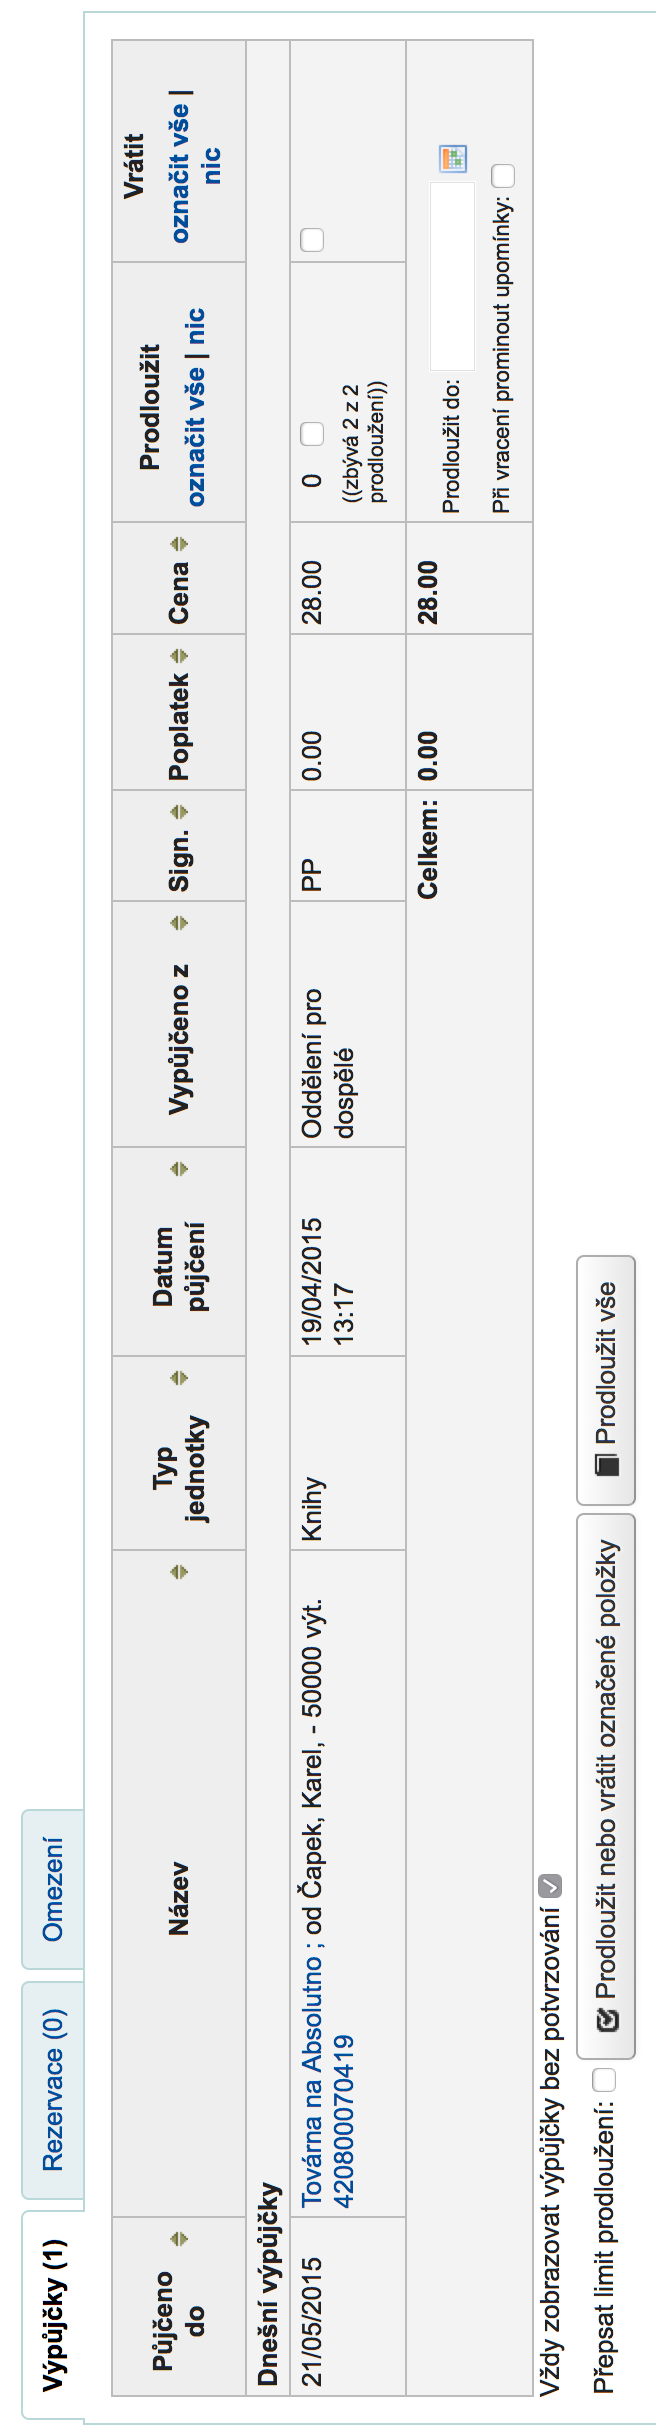
\includegraphics[width=0.5\textwidth]{resources/vypujcky_left}
    \caption{Výpůjčky čtenáře v~systému Koha}
    \label{vypujcky}
\end{figure}

Koha umí uživatele předem notifikovat pomocí emailu nebo SMS, kde správa šablon různých zpráv je samozřejmostí. Těmto notifikacím lze různě nastavovat například periodicitu a~další vlastnosti.

\subsubsection{Napojení na selfchecky}
Koha podporuje protokol SIP2, díky kterému je možné napojit systémy selfchecků, RFID technologie, kopírky/tiskárny či Zebra tiskárny pro tisk štítků.% #TODO add citation Choosing free library software: Experiences of the Faculty of Humanities and Social Studies in Zagreb, s. 651

\subsubsection{Podpora více výpůjčních protokolů}
Jelikož má Koha možnost vytvářet pobočky, má i podporu více výpůjčních protokolů. V~systému Koha je možné nastavovat vazby mezi jednotlivými knihovnami/pobočkami, tudíž je možné nastavit, kdo má na co práva a~kam „vidí“. Je tedy možné pobočky propojit nebo naopak rozdělit.

\subsubsection{Lokální a~globální karty Alephu}
Tato funkcionalita vyžaduje hlubší šetření. Momentálně se databáze uživatelů sdílí mezi všemi v~rámci instance a~jde blokovat jen globálně a~to buď na základě poplatků nebo nevrácení. V~případě, kdy by v~rámci instance neměla knihovna vidět do uživatelské databáze jiné knihovny, je potřeba chování systému upravit. Bylo by tedy potřeba vytvořit testovací instanci, která by představovala novou strukturu systému a~na ní odladit potřebné požadavky.

\subsubsection{MVS (Meziknihovní výpůjční služba)}
Meziknihovní výpůjční služba funguje v~Koha jako běžná výpůjčka, ale pro speciální typ uživatele - knihovnu. Knihovny jsou speciální kategorie čtenářů s~odpovídajícími parametry, jako cena za nula a~pravidly pro výpůjčky. Takže se provede klasická výpůjčka, která se následně odešle poštou. Lze vygenerovat report, který přehledně zobrazí, jaká knihovna od kdy má daný dokument. Příchozí MVS je řešena specifickým typem dokumentu, který má nastaven kratší dobu výpůjčky, navěšeno hlášení při návratu a~specifickou katalogizační šablonu. Takže dokument je přijat, rychle zkatalogizován, do jednoho pole je zapsáno, od koho je, a~půjčen čtenáři. Opět je k~dispozici report, který vypisuje, jaké dokumenty v~rámci příchozích MVS jsou k~dispozici, kdo je má, atd. Toto fungování nemusí zcela vyhovovat MU a~celou agentu bude pravděpodobně potřeba upravit nebo použít MVS modul\footnote{ILL modul Koha - https://github.com/PTFS-Europe/koha/tree/ill\_master}.

\subsection{Potřeby a~požadavky uživatelů}
Celý problém lze rozdělit na dvě části, vnitřní a~vnější. Tou vnitřní částí je rozhraní systému, se kterým měli potíže zaměstnanci. Tento problém lze v~systému Koha vyřešit velmi elegantně a~prakticky bez bariér. Jelikož je rozhraní systému webové, lze ho upravovat pomocí technologií HTML5 a~CSS3 spolu s~JavaScriptovou knihovnou jQuery, která dodá celému rozhraní uživatelskou přívětivost (efekty místo statického loadingu, asynchronní načítání obsahu, hezké zobrazování notifikací, slideUp efekty místo klasického smazání části obsahu a~mnoho dalšího). Právě JavaScript je jednoduché řešení, po kterém knihovny sahají, potřebují-li si přizpůsobit nějaké řešení svým potřebám. \citepages{80-82}{Denar2015thesis} Do každé stránky rozhraní lze vkládat libovolný javascript, takže upravit lze prakticky všechno. Díky jQuery lze tedy definovat  vlastní události a~přiřazovat k~nim nové či pozměněné akce nebo měnit či přidávat efekty. \citepages{3-9}{IYiYMQHMhgWYsu4q}

Vnější část problému je uživatelské rozhraní, tedy OPAC\footnote{Online Public Access Catalog
}, se kterým uživatelé neumí pořádně pracovat. Při provádění výzkumu měl autor studie možnost vyzkoušet si práci referenčního knihovníka na Filozofické fakultě Masarykovy univerzity, z~čehož vyplynulo, že uživatelé OPACu opakovaně nebyli schopni dohledat informace, které potřebovali, a~žádali o~pomoc referenční knihovníky. Většinou to byly problémy jako nedohledatelná kniha na regálu, nemožnost inteligentně dohledat knihu na nějaké téma v~ruském jazyce a~podobně.

Problém s~jazyky byl ten, že OPAC nabízel například 3 jazyky z~určitého MARC pole, zatímco se reálně prohledávalo pole jiné. V~době psaní této práce existovala někde v~rozhraní tabulka se zkratkami jazyka, které bylo možné použít pro prohledávání. Uživatelé, kteří o~tabulce nevěděli, byli nuceni zvolit jeden z~jazyků, spustit vyhledávání a~v~URL změnit zkratku jazyku za jinou, kterou si tipli, že je správná pro daný jazyk.

Tyto problémy lze v~systému Koha vyřešit zaprvé správným zaindexováním dat a~zadruhé uživatelsky přívětivým OPACem, kterým se osvědčil být VuFind vyvíjený jako open source na Villanova University. \citepages{12}{Coufalova2009} Tento OPAC používá drtivá většina knihoven v~České republice provozující systém Koha (zbytek knihoven je maximálně nenáročných a~zůstali na interním Koha OPACu). VuFind umožňuje uživatelům vyhledávat v~celém fondu knihovny a~nabízí i doplňkové služby a~to celé přehledně a~jednoduše. VuFind je modulární, o~čemž svědčí i fakt, že je na něm postaven český Centrální portál knihoven\footnote{Centrální portál Knihoven (CPK) - https://knihovny.cz/}, který poskytuje přístup k~fondům a~službám všech zapojených knihovních i neknihovních institucí v~rámci republiky. Centrální portál knihoven je vyvíjen jako open source a~jeho moduly jsou dostupné v~repozitáři na Githubu\footnote{CPK repozitář https://github.com/moravianlibrary/VuFind-2.x
}. Lze se tak inspirovat řešením, které prošlo uživatelským testováním a~je založeno na uživatelsky přívětivém moderním designu. \citesource{aktivity_2016}  \citesource{smlouva_o_dilo_2015}

VuFind je navíc discovery systém, který lze v~rámci Masarykovy univerzity využít k~zapojení externích elektronických informačních zdrojů, což OPAC Kohy neumožňuje. VuFind je také stavěný na práci se Solrem, což je databázový systém vhodný pro práci s~Big Data. Podle Alfreda Serafiniho\footnote{Freelance software konzultant, autor publikace Apache Solr Beginner's Guide (ISBN 978-1-78216-252-0).} je to vhodný nástroj pro prohledávání velkého množství read-only metadat, kde jako příklady využití uvádí právě VuFind a~Internet Archive\footnote{Internet Archive - http://www.archive.org/}. \citepages{20}{68071520130101}

Idea rozhraní VuFind je založena na teorii, že uživatele nezajímá cesta, jakou se k~dokumentu dostane, ale v~jaké formě je k~dispozici a~jak je možné ho získat v~rámci instituce. \citepages{20}{Coufalova2009} Lze tedy tvrdit, že katalog, který slouží knihovníkům, nemůže být stejný jako OPAC \citepages{5}{Schmidt2012}, jelikož ten má být designován pro uživatele, kteří s~ním interagují. OPAC je veřejnou částí knihovního systému, tedy vstupní bránou uživatele, která musí být uživatelsky přívětivá, musí tedy splnit potřeby uživatele, které lze vydefinovat pomoci Maslowovy pyramidy webdesignu \citepages{156-179}{rezac_2014}, kam patří důvěryhodnost, radost z~používání, vytvoření vazby, přesvědčivost, použitelnost, přístupnost, dostupnost, nalezitelnost a~smysluplnost. 

Tak jako Koha, i VuFind je postaven na webových technologiích, což dává designerům a~softwarovým architektům obrovské možnosti v~rámci přizpůsobení veřejného rozhraní. Pomocí HTML5 lze rozhraní zpřístupnit i zrakově či jinak handicapovaným uživatelům, kterým se tak OPAC zpřístupní pro jejich speciální čtecí zařízení. \citepages{19-27}{Hogan2011}

Zajímavostí je také budoucnost těchto technologíí, která vnáší do oboru knihovnictví sémantičnost v~rámci webového rozhraní. Díky HTML5 a~sémantickým technologiím, jako je například mikroformát RDF (a také samotná podstata sémantiky v~HTML5), je možné dávat jednotlivým částem webu význam, což z~něho dělá lépe prohledávatelný web na Internetu, na což vzápětí navazuje i chytré vyhledávání na webu za využití umělé inteligence. \citepages{70-77}{fay_sauers_2012} Takto lze OPAC připravit na budoucnost webu 3.0, respektive webu 4.0.

VuFind je navíc založen na myšlence responsivního designu a~využívá webového frameworku  Bootstrap 3, je tedy responzivní ve smyslu přístupnosti na zařízeních s~různou uhlopříčkou a~rozlíšením, takže je stejně použitelný jak na desktopech, tak i na tabletech či smartphonech.

\subsubsection{Služba Copy on Demand (COD)}
Tato služba přímo v~Koha ani ve VuFindu neexistuje, avšak je natolik triviální, že její napsání nezabere víc jak pár hodin. Tuto funkci lze také řešit externí službou, která vygeneruje odkaz (tlačítko), který stačí jednoduše embedovat\footnote{Vložit.} do šablony OPACu.


\subsubsection{Obálky knih}
Nejen obálky knih, ale i naskenované obsahy a~indexy lze zpřístupnit ve VuFindu pomocí API ObálekKnih\footnote{API ObálkyKnih.cz - https://obalkyknih.cz/doc/Dokumentace\_API\_OKCZ\_3.1.pdf.} ve verzi 3. Příklad implementace ve VuFindu lze vidět na Centrálním portálu knihoven, respektive v~repozitáři\footnote{Implementace ObálekKnih v~CPK https://github.com/moravianlibrary/VuFind-2.x/tree/master/themes/obalkyknih-api-v3-bootstrap3} na Githubu.

\subsubsection{Automatická oprava překlepů a~nabídka alternativ při neúspěšném hledání}
Tuto funkcionalitu lze zapnout vyhledávací komponentou \code{spellcheck}.

\subsection{Systémové požadavky} \label{sec:systemove_pozadavky}
Následující část rozebírá hlavní systémové požadavky na knihovní systém Masarykovy univerzity.

\subsubsection{Velký počet knihovních jednotek, uživatelů, poboček, podpoboček}
V~této chvíli je potřeba, aby nový systém zvládl cca 2 miliony knihovních jednotek, cca 50 000 aktuálně registrovaných  uživatelů.

Toto kritérium by nemělo být problémem, jelikož např. síť 900 aktivních knihoven v~Turecku (z~celkového počtu 1 126) obsluhuje 13 700 000 knihovních jednotek a~1 220 000 aktivních uživatelů v~jedné instalaci systému Koha. \citesource{koha_komunita_2016}
 Používají na to 14 produkčních serverů, 4 testovací, MariaDB a~Galera Cluster se čtyrmi nody, 8 Apache serverů a~jeden Zebra server. 

Koha je navíc škálovatelná\footnote{Schopnost systému pružně reagovat na vzrůstající nebo klesající nároky uživatelů na výkon systému.}, lze tedy tvrdit, že počet obsloužených jednotek a~uživatelů je záležitost technická. Toto škálování (horizontální i vertikální) \citepages{1-4}{6847479} je možné provádět například pomocí open source produktů OpenStack a~OpenShift společnosti RedHat. 

OpenStack řeší infrastrukturu (infrastructure as a~service - IaaS), to znamená poskytování bootovatelného virtuálního stroje, networkingu, datového úložiště a~dalších. \citepages{14-16}{breeding_2012} OpenShift jako platforma (platform as a~service - PaaS) zase řeší rychlý deploy LAMP\footnote{Linux, Apache, MySQL/MariaDb, PHP/Perl/Python.} aplikací.

\subsubsection{Flexibilita}
Jedním ze základních požadavků na knihovní systém v~knihovnách Masarykovy univerzity je vysoká potřeba vše členit do složitějších hierarchických struktur (uživatelé, katalogy, pobočky). Velké univerzity nemají typicky jednu knihovnu, ale celou síť navzájem propojených knihoven, kterou musí být systém schopny obsluhovat jednotně a~současně podporovat jejich odlišnosti. Masarykova univerzita má 10 fakultních knihoven, které momentálně operují nad společným systémem/katalogem, fungují však do značné míry samostatně. Mají odlišné zejména otevírací doby, statusy knih, výpůjční doby a~pokuty, akvizice a~fakturace jednotek. Společnou však mají centrální bázi uživatelů s~možností lokální registrace na pobočkách. 

Důležitá je také podpora konsorcií. Celá Masarykova univerzita se chová svým způsobem jako konsorcium. Kromě toho ale může nastat případ, kdy instalovaný systém bude potřeba provozovat skutečně pro více různých nezávislých institucí - konsorcium.

Velká flexibilita je potřebná prakticky ve všem, například při propojování záznamů při zpracování specifických typů dokumentů (přítisky, přívazky, monografická čísla a~podobně).

Při současném řešení je nutné řešit vícero samostatně prohledávatelných knihovních databází (s~možností dalšího členění do dílčích knihoven a~studoven) a~souborný katalog pro celou univerzitu.

Z~pohledu systémové vrstvy existují při instalaci systému Koha tři možnosti:

\begin{itemize}
\item samostatná instalace pro každou knihovnu
\item jedna instalace a~instance pro každou knihovnu
\item jedna instalace a~knihovny jako jednotlivá oddělení (některá mohou být nezávislá - nevidí zbytek)
\end{itemize}

Samostatná instalace je nezávislá ve všech směrech.
Instalace pro jednotlivé knihovny mohou zjednodušit správu, protože vše běží na jednom serveru. To znamená, že aktualizace a~správa systému se dělá jen jednou. Navíc je využita jedna databáze, takže existuje teoretická možnost automatizované synchronizace subdatabází jednotlivých instancí. \citepages{19-21}{breeding_2012}

Jednou z~možností, které by nejvíce vyhovovaly stávající architektuře systému Aleph a~systémům, které je potřeba zapojit, se jeví schéma na obrázku \ref{fig:koha}. Finální návrh struktur instalace však vyjde až z~kompletních informací ohledně rozdělení jednotlivých knihoven a~poboček a~požadavků na jejich samostatnost a~začlenění do skupin a~hierarchie.

\begin{figure}
    \centering
	\def\svgwidth{1.27\textwidth}
    \input{koha.pdf_tex}
	\caption{Možná akrchitektura systémů MU při využití open source řešení Koha.}
	\label{fig:koha}
\end{figure}

\subsubsection{Robustnost a~vysoká provozní spolehlivost systému}
Tak robustní systém jako ILS pro MU může být náchylný k~výpadkům, spravuje-li velké množství dat a~dotazů. Tomu je potřeba zabránit nebo to alespoň omezit na minimum. V~případě výpadku sítě či napájení je nutné systém obnovit ze zálohy, aniž by došlo k~poruše konzistence či integrity dat.

Systém musí fungovat non-stop. Při problémech způsobených nějakou vstupní chybou nesmí tyto chyby způsobit výpadek systému nebo porušit integritu dat \citepages{2}{bartosek_2001_systemovy_pohled} a~tyto chyby/výjimky musí být korektně odchytávány a~ošetřovány. S~provozní spolehlivostí také souvisí výkon. Důležitým aspektem je jak rychlá odezva, tak rychlé zpracování velkého množství dat. O~škálování systému se již psalo v~kapitole \ref{sec:systemove_pozadavky} Systémové požadavky, avšak je potřeba myslet i na to, že neustále zvyšování nároků na výpočetní výkon také zvyšuje nároky na koncové stanice uživatelů \citepages{2-3}{bartosek_2001_systemovy_pohled}.

Koha také plně podporuje technologii PSGI/Plack, která slibuje zrychlení většiny každodenních úkonů. \citesource{koha_3.22_released_2016}
 PSGI je rozhraní mezi perlovskou aplikací a~serverem, zatímco samotný Plack je perlovským modulem a~nástrojem, který obsahuje PSGI middleware, helpery a~adaptery pro web server.  \citesource{psgi/plack_2016}

\subsubsection{Otevřenost systému}
Systém musí být technicky připraven na to, aby mohl být napojen na další systémy využívané v~rámci Masarykovy univerzity, tj. personální, ekonomický, studijní.

Celkově fakt, že Koha je open source systém, dává případnému napojování na další systémy velké možnosti, jelikož je možné do kódu zasahovat a~přizpůsobovat si tak knihovní systém svým potřebám, aniž by knihovna musela žádat výrobce o~novou funkcionalitu.

V~případě, že jiná knihovna již tento krok podstoupila, je možné v~rámci komunity tento kód  implementovat i do forku (derivátu repozitáře) \citepages{29}{Chaconc2009} té dané knihovny, tudíž není potřeba znovu vyvíjet software s~ekvivalentní funkcionalitou nebo nesmyslně platit za již zaplacenou věc. Knihovna samozřejmě nemusí mít vlastní fork a~může přispívat do upstreamu (zdrojový repozitář), odkud si Kohu vzala, tudíž sdílí novou funkcionalitu s~komunitou.

V~případě, že organizace má vlastní vývojáře, je rychlost vývoje OSS rychlá a~relativně bezproblémová a~navíc projde kód kontrolou nejen formální (kód samotný), ale i věcnou (zakomponování do zbytku systému). OSS reaguje na požadavky uživatelů, kdežto proprietární software nabízí funkcionality na základě své strategie nebo obchodního modelu. Některé funkce tak díky vysokým nákladům nemusí být nikdy implementovány, výrobcům se zkrátka nevyplatí. Pokud se mu tyto části funkcionality mají vyplatit vyvíjet, nasadí podle toho i jejich cenu. Výsledkem jsou služby, které si některé knihovny nemohou dovolit, což má vliv na jejich začlenění do kooperativních projektů nebo na kvalitu a~rozsah poskytovaných služeb.

\subsubsection{Bezpečnost systému}
Bezpečnost systému lze uvažovat nejméně ze tří úhlů pohledu. První úroveň uvažuje bezpečnost v~rámci přístupu do systému a~jeho částí (autentizace). Druhá úroveň uvažuje bezpečnost týkající se pravomocí jednotlivých skupin uživatelů (autorizace). U~těchto úrovní se dá mluvit jako o~prevenci zneužití či poškození dat, ať už úmyslného nebo ne. Třetí úroveň lze uvažovat jako logovací, neboli zaznamenávající chování v~systému. Veškerá bezpečnost se týká aplikační vrstvy ISO/OSI \citepages{80-82}{kurose_ross_2014} modelu počítačové sítě.

V~Koha se připravuje balíčková podpora LetsEncrypt, takže bude poměrně snadné přejít na HTTPS. Pravidelně se řeší bezpečnostní aktualizace (minimálně 1x/měsíc). Hesla jsou šifrována pomocí Bcryptu.

\subsubsection{Shibboleth}
Napojení na open source federativní sytém pro propojování identit Shibboleth je také možné a~konfigurace je dostupná na wiki stránkách\footnote{Konfigurace Shibbolethu pro Koha - https://wiki.koha-community.org/wiki/Shibboleth\_Configuration} mezinárodní komunity.

\subsubsection{Dokumentace}
Jedním z~požadavků byla dostupná plná dokumentace systému. Pro systém Koha je k~dispozici:

\begin{itemize}
\item dokumentace systému\footnote{Dokumentace Koha - https://koha-community.org/documentation/}
\item dokumentace k~veškerým API a~podporovaným protokolům\footnote{API a~protokoly Koha - \url{https://wiki.koha-community.org/wiki/APIs\_and\_protocols\_supported\_by\_Koha}}
\item český manuál \footnote{Český manuál Koha - http://www.knihovni-system-koha.cz/index.php/navody-a-vzdelavani/cesky-manual-systemu-koha}
\end{itemize}

\subsubsection{Externí aplikace knihoven}
Následující externí aplikace knihoven lze řešit přímo knihovním systémem.

\begin{itemize}
\item \bold{Dlouhodobé výpůjčky, které letos končí} (KUK) - toto by měla zvládnout pravidla výpůjček. Ta se definují od obecných ke specialitám. Buď podle typu dokumentu nebo kategorie čtenáře, nebo knihovny. Upozornění pak chodí automaticky.
\item \bold{Hromadná objednávka} (KUK) - možnost vytisknout více titulů do jednoho objednávkového formuláře. V~tomto případě stačí nadefinovat design MU.
\item \bold{Rozpočty} - přehled rozpočtů, čerpání financí (KUK).
\item \bold{Limity nákupů} (KUK).
\item \bold{Přehled fondů pro potřeby akreditací} - vygenerování přehledu počtu svazků knih/časopisů podle majetku fakulty a~kolik z~toho je ve volných výběrech (KUK). V~systému Koha lze řešit jako statistiky na základě metadat.
\item \bold{Kontrola řady čárových kódů} – při zpracování knih se občas ztratí čárový kód, je potřeba ho dohledat a~obsadit (jeho číslo je zároveň přírůstkové číslo) (KUK).
\item \bold{Kontrola chyb} (KUK) - v~Koha existuje celá řada chybových kontrol, které lze spouštět ručně nebo je automatizovat.
\item \bold{Dopis hříšníkům} (KUK).
\end{itemize}

\subsection{Potřeby a~požadavky katalogizace}

Katalogizační modul Kohy samozřejmě podporuje správu digitálních informačních artefaktů a~má i možnost vytvářet nové multimediální materiály. Modul disponuje přehledným katalogizačním editorem, který lze snadno editovat. Záznamy lze dotahovat přes Z39.50/SRU\footnote{Search/Retrieve via URL.}. 

Je možné vytvářet vlastní MARC šablony pro různé typy dokumentů. Položky, které se často opakují, či dlouhé seznamy možností je možné definovat do tzv. ověřených hodnot. Tyto ověřené hodnoty se pak zobrazí v~šabloně v~podobě roletek, ze kterých je možné vybírat.

Národní autority se v~Koha dotahují přes Z39.50 (v~knihovnách MU pomocí FTP\footnote{File Transfer Protocol - protokol pro transport dat.
.}). OAI harvester je pro Kohu ve fázi implementace.

Editor lze rozdělit do záložek 0-9, které definují rozsah polí, viz. obrázek \ref{fig:editor}. Tyto záložky lze slovně pojmenovat nebo rozhraní zobrazovat jako celý záznam.

\begin{figure}
    \centering
    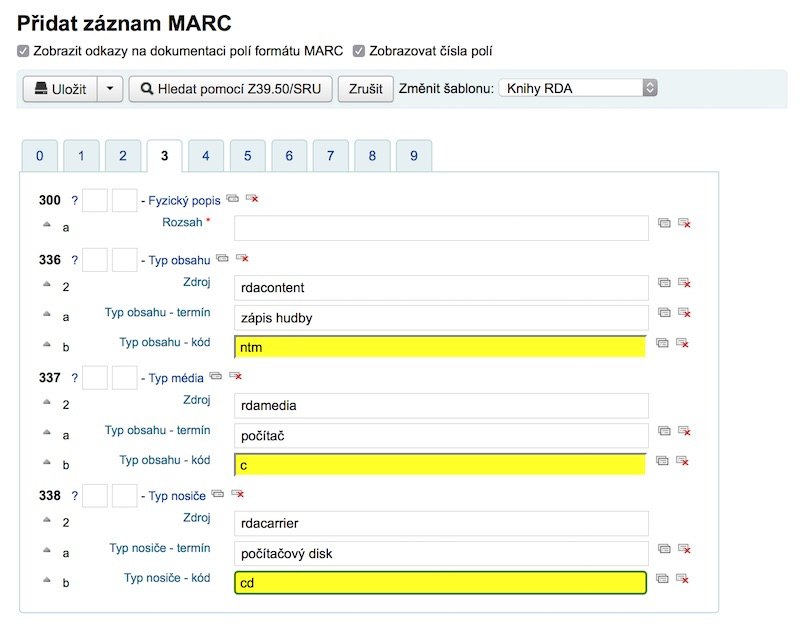
\includegraphics[width=1.0\textwidth]{resources/katalogizacni_editor}
    \caption{ }{Katalogizační editor systému Koha\protect\footnotemark}
    \label{fig:editor}
\end{figure}
\footnotetext{Katalogizační editor systému Koha - http://www.knihovni-system-koha.cz/index.php/projekty/podpora-rda}

\subsubsection{Hromadné úpravy}
Záznamy lze editovat také hromadně pomocí nástroje „Hromadné úpravy jednotek“, kde se nadefinují modifikační šablony, viz obrázek \ref{fig:hromadne_upravy}.

\begin{figure}
    \centering
    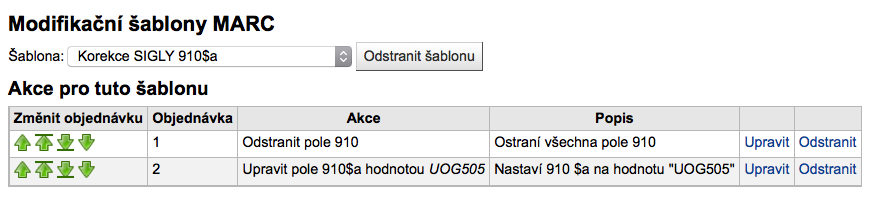
\includegraphics[width=1.0\textwidth]{resources/hromadne_upravy}
    \caption{Hromadné úpravy záznamů v~systému Koha}
    \label{fig:hromadne_upravy}
\end{figure}

Co se katalogizace elektronických zdrojů týče, elektronické zdroje se katalogizují jako knihy, jen se použije jiná šablona. Rozdíl v~záznamu je primárně v~kódovaných údajích.

\subsubsection{Podpora RDA}
Hezkým příkladem, jak lze upravovat frontend za využítí Javascriptu, je úprava bibliografických a~autoritních šablon pro podporu RDA, kde jsou jednoduše vložena chybějící pole a~možnost zobrazovat hodnoty, které lze do polí vložit.

\subsubsection{Stahování bibliografických záznamů přes Z39.50}
Koha podporuje protokol Z39.50 jako klient i jako server, to znamená, že dokáže stahovat záznamy například z~Národní knihovny, Jednotné informační brány, Souborného katalogu, Moravské zemské knihovny a~podobně, ale také povoluje jiným knihovnám stahovat své záznamy (například v~rámci konsorcia).

\subsubsection{Rejstříky}
Koha umí pracovat s~čímkoliv, co má povahu autority (korporace, věcné téma, místo, žánr) a~také umí vytvořit řízený slovník čehokoli, co má pak povahu oveřených hodnot, které lze provázat s~katalogizační šablonou.

\subsubsection{Omezení práv}
V~Koha lze udělovat práva pro to, který personál má mít přístup k~editaci jednotek a~který k~editaci záznamů. To znamená že někteří zaměstnanci nemohou editovat záznam, ale mohou jenom změnit například čárový kód, a~podobně. Slouží k~tomu komponenty \code{SubfieldsToUseWhenPrefill} a~\code{SubfieldsToAllowForRestrictedEditing}.

\subsubsection{Autoritní hesla}
Výběr autoritních hesel je pro Kohu samozřejmostí. Možnost dohledat autoritu zobrazuje obrázek \ref{fig:vysledky_vyhledavani_autorit}.

\begin{figure}
    \centering
    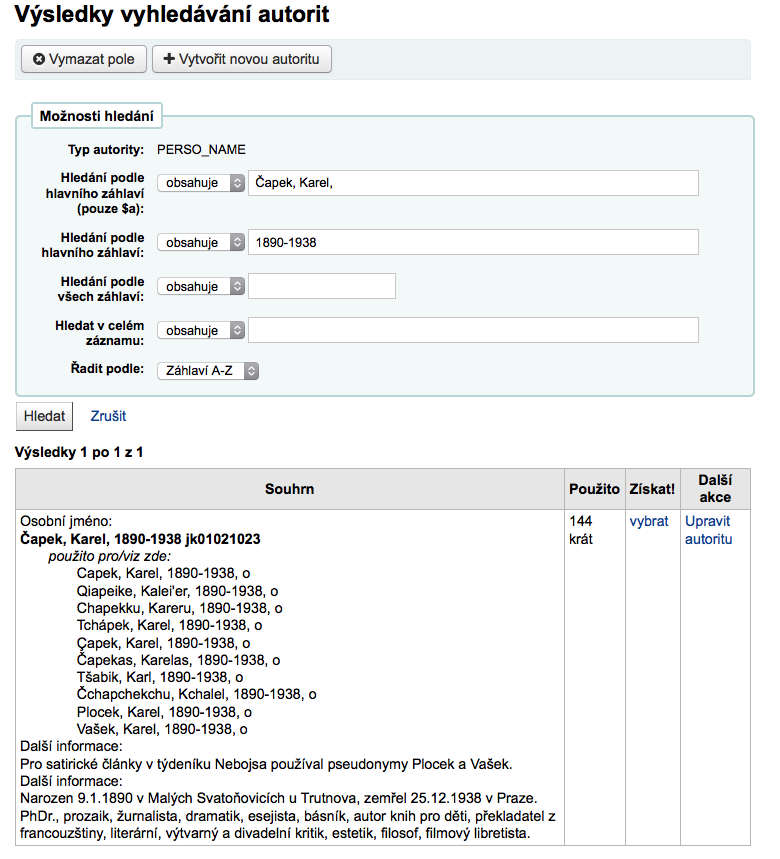
\includegraphics[width=1.0\textwidth]{resources/vysledky_vyhledavani_autorit}
    \caption{Výsledky vyhledávání autorit v~Koha}
    \label{fig:vysledky_vyhledavani_autorit}
\end{figure}

\subsection{Potřeby a~požadavky akvizice}
Modul akvizice disponuje běžnými funkcemi, které jsou pro procesy akvizice v~knihovnách potřeba, to znamená, že Koha dokáže vytvářet dodavatele, aplikovat slevy, rozlišovat ceny s~DPH a~bez DPH a~podobně. Tyto údaje tedy pomáhají při příjmu objednávky, kdy lze jednoduše zkontrolovat fakturu. Objednávku lze vyvářet jednoduše, a~to vytvořením jednoho nebo více košíků, kde se pro každého dodavatele navolí jednotlivé položky objednávky. Záznamy těchto položek lze doplnit buď z~vlastní databáze, nebo dotáhnout přes Z39.50 například z~České národní bibliografie nebo Souborného katalogu.

Jedním z~požadavků bylo, aby nový systém uměl evidovat adresy dodavatelů, IČ a~DIČ, což pro Kohu není problém.

V~systému Koha je také možné dohledat, kolik knih bylo koupeno a~z~jakých zakázek. Ke každému dodavateli jsou přiřazené objednávky. Když se uzavřou, je možné je exportovat do tabulkového formátu nebo PDF. Ve vygenerované tabulce lze označovat, které položky objednávky v~balíku dorazily, a~tedy vidět, které položky nebyly pokryty. Takto se vytvoří seznam dokladů, ke kterým se přiloží naskenovaná faktura. Částky se odepíšou z~rozpočtů, které mohou mít různé složky a~fondy. Koha sama sleduje vykrytí, má jednoduché predikce plnění a~upozotňuje, když se přibližuje k~vyčerpání částky nebo procentuální části. Příklad objednávky lze vidět na obrázku \ref{fig:objednavka}.

\begin{figure}
    \centering
    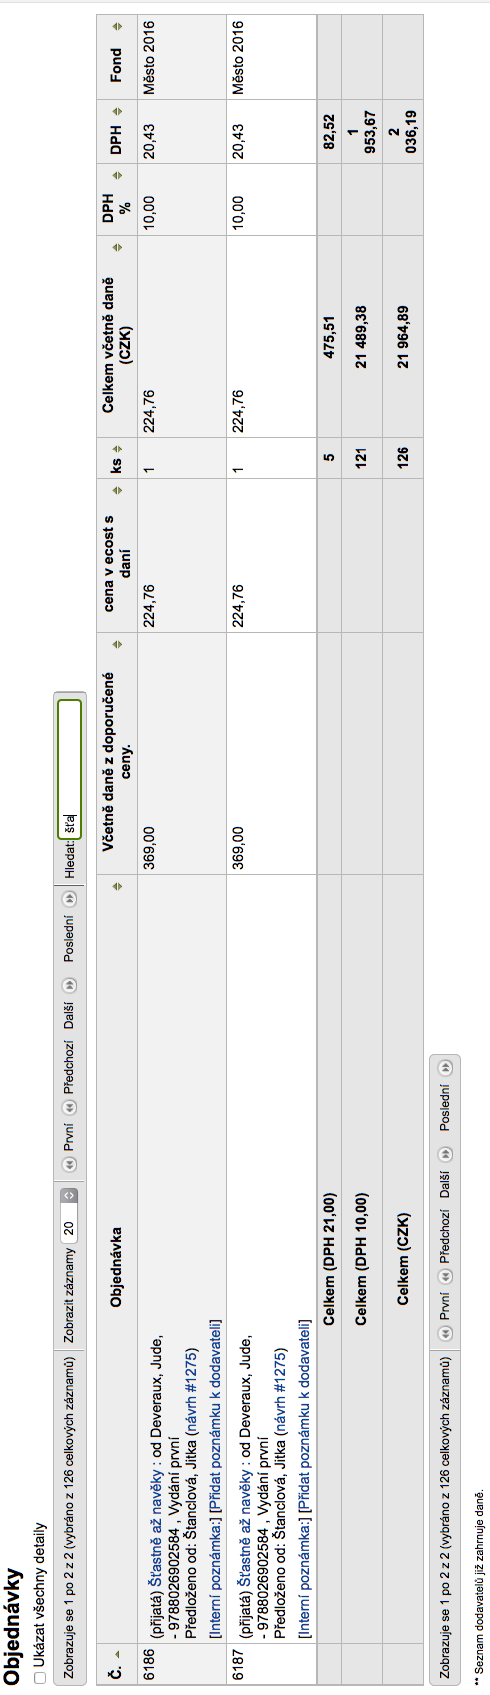
\includegraphics[width=0.5\textwidth]{resources/objednavka_left}
    \caption{Příklad objednávky v~systému Koha}
    \label{fig:objednavka}
\end{figure}

\section{Dopad projektu na životní prostředí}
Systém Koha je napsán v~perlu, neupovídaném stručném skriptovacím jazyce \citepages{v-ix}{Wall1997}, což má za následek také menší celkovou velikost zdrojového kódu. To vede k~menší náročnosti na zpracování na straně serverů a~menší energetickou zátěž, tudíž lze tvrdit, že více šetří životní prostředí. Jak tvrdí motto jQuery, který využívá Koha i VuFind: \citace{Write less, do more}. \citesource{jquery_2016}

\section{Finanční plán a~ekonomická analýza projektu}
Při řešení finanční otázky projektu je potřeba myslet zejména na to, že finance ušetřené na koupi nebo podporu systému bude nutné vložit do mezd personálu, který bude migraci provádět. Tento projekt bude realizován několik měsíců a~v~každé etapě bude potřeba jiné skupiny lidí. Tyto lidské zdroje však budou v~plném nasazení potřeba jen ze začátku, kdy se bude migrovat a~pak systém kustomizovat. Poté náklady na pracovní skupiny klesnou na potřebnou systémovou podporu, která se bude starat o~chod a~správu systému.

Ve chvílích, kdy bude potřeba psát nové funkce či upravovat ty stávající, je vhodné je konzultovat s~komunitou. To z~toho důvodu, že bude-li mít o~funkcionalitu zájem více institucí, mohou se náklady rozdělit mezi zájemce v~komunitě, a~to jak finanční,  tak i ty lidské.

\section{Hodnocení efektivity a~udržitelnosti projektu}
Celé hodnocení efektivity a~udržitelnosti projektu ve velké míře závisí na tom, jak se případný objednatel (v~tomto případě MU) postaví k~výsledkům SWOT analýzy a~jak využije silné stránky a~jak se vypořádá se slabými stránkami projektu. Následující SWOT analýza byla prováděná v~průběhu 6 měsíců a~probíhala současně s~průzkumem mapování knihovních procesů v~MU. Hlavním předmětem analýzy byla migrace na open source systém Koha. Analýza byla prováděna jako instalace nové Kohy, vytvoření instancí a~následného dohledávání externí podpory, rozhovorů s~knihovníky a~systémovými knihovníky MU, Ústavem výpočetní techniky a~knihovnami, které migrací prošly bud samostatně nebo s~využitím externí komerční podpory. Analýza je zpracována ke dni 07. 03. 2015 a~její životnost se odhaduje na 5 let (v~případě její další revize).

\begin{table}
    \centering
    \begin{tabular}{ p{5.8cm} | p{5.8cm} }
    \bold{Silné stránky (S)} 
    \begin{itemize}
		\item open source
		\item webový klient systému
		\item nastavení systému „na míru“ potřeb dané knihovny
		\item úspora nákladů na pořízení a~provoz systému (sdílení nákladů na vývoj, provoz)
		\item žádný vendor lock-in
	\end{itemize}
    & 
    \bold{Slabé stránky (W)} 
    \begin{itemize}
		\item nelze srovnat s~jinou migrací v~rámci ČR v~posledních letech
		\item nutnost dopsat chybějící funkcionalitu
		\item nutnost upravit moduly k~potřebám knihoven
		\item obava o~zvládnutí přechodu a~údržby systému svépomocí
	\end{itemize}
    \\ \hline
    
    \bold{Příležitosti (O)} 
    \begin{itemize}
		\item možnost centralizovat služby pro uživatele, discovery systém a~OPAC
		\item možnost zapojení se do komunity
		\item možnost zapojit studenty do tvorby chybějící funkcionality nebo možnost vytvořit předmět s~praktickým výstupem zaměřený na vývoj open source softwaru na vybraných projektech
		\item komplexnější pochopení procesů v~knihovně knihovníky
		\item vytvoření nové úrovně a~formy spolupráce mezi knihovnami
		\item součásti přechodu lze optimalizovat procesy v~knihovnách
	\end{itemize}
    & 
    \bold{Hrozby (T)} 
    \begin{itemize}
		\item neochota zaměstnanců učit se s~novým systémem
		\item možnost, že se projeví neznalost problematiky v~oboru knihovnictví jeho zaměstnanci
		\item možnost nedokončení migrace v~případě nepevného vedení všech etap celého procesu
	\end{itemize}
    \end{tabular}
    \caption{SWOT analýza projeku migrace na open source systém Koha v~knihovnách MU}
\end{table}

Udržitelnost projektu, který by byl zrealizován, je závislá na mnoha faktorech. Jedním a~zároveň tím nejzásadnějším je způsob vývoje a~udržování systému. Systém je totiž možné provozovat tak, že se vyklonuje\footnote{Pořídí kopie.} vzdálený Koha repozitář z~upstreamu\footnote{Zdrojový repozitář verzovacího systému.}, do kterého v~budoucnu bude možné jednoduše stahovat\footnote{Stahovat - pullovat nové verze dat z~repozitáře. Opakem pullu je push, kdy se to repozitáře vkládají nové verze dat.} aktualizace z~upstreamu. Druhá cesta je vytvořit kopii vzdáleného repozitáře a~vývoj dělat v~rámci svého forku. To sebou nese jak výhody, tak i nevýhody. Hlavní výhodou je, že změny, které se udělají ve forku, nebude nutné procházet zdlouhavým code review na straně Koha komunity, což má za následek i to, že MU nebude závislá na tom, zda novou funkcionalitu komunita zařadí do standardního balíčku v~master větvi\footnote{Hlavní větev v~repozitáři verzovacího systému Git.} repozitáře. Tento krok však může MU využít, bude-li se jednat o~nějakou všeobecnou univerzální funkcionalitu. 

Bude-li to lokální záležitost, může to provozovat ve svém forku a~o~nic se nestarat. Tato varianta se jeví jako nejvhodnější, ale je potřeba počítat s~tím, že bude-li chtít MU stahovat aktualizace z~upstreamu, mohou nastat konflikty v~kódu, které bude potřeba řešit ve smyslu slučování\footnote{Situace, kdy je potřeba spojit 2 verze souboru, se nazývá merge.} dvou rozdílných verzí souboru. Třetí cesta je pak, že MU naklonuje Koha repozitář, který již nebude slučován s~upstreamem, tedy úplně se odřízne od upstreamu. Toto řešení však není vhodné kvůli budoucí správě systému v~případě, kdy by MU chtěla externí pomoc a~verze Kohy a~upstreamu by se hodně lišila. 

\section{Analýza a~řízení rizik}
V~průběhu provádění všech etap a~hlavně po celkovém ukončení realizace je potřeba mít možnost poskytnutí zpětné vazby a~fungující komunikaci v~celém konsorciu. V~kterékoliv z~etap realizace projektu mohou nastat problémy, které je vhodné řešit co nejdříve, aby nedošlo k~dalším komplikacím. Celá realizace stojí a~padá také na vedení a~proto je nutné, aby v~případě problémů vedení tyto problémy diskutovalo a~řešilo. 

Může nastat situace, kdy se změní směřování ústavu a~open source již nebude hlavní myšlenkou dne. V~tom případě se při nejhorším ztratí čas a~úsilí věnované projektu (s~tím spojené i mzdové náklady). Knihovny však nebudou jinak zasaženy a~budou fungovat stávajícím způsobem. Je vhodné migraci, respektive implementaci nového systému, provádět na testovacích serverech a~data importovat do testovacích databází, aby se zabránilo případným nechtěným kolizím.

Další riziko představuje fakt, že problémy, které MU měla při stávajícím systému, přetrvají i po migraci na Kohu. V~tom případě problém nebyl knihovní systém, ale špatná komunikace, nastavení nebo procesy.

Rizikem může být i to, že nový systém přinese mnoho změn, které se v~tak konzervativním prostředí, jako je knihovnictví, těžko uplatňují. V~tomto případě je dobré věnovat náležitou pozornost plánu přechodu a~školení. To by se nemělo týkat jen nového systému jako takového, ale i procesům v~knihovně.

Finanční riziko zase představuje neušetření financí (alespoň na začátku) při migraci na open source. Důvodem může být využití ušetřených prostředků na mzdách pracovníků, kteří budou nový systém upravovat a~nastavovat. 

Riziko může také nastat v~době, kdy budou knihovníci muset vývojářům a~systémovým knihovníkům definovat, jak má která služba fungovat nebo jak se mají data interpretovat. Může se stát, že to ve skutečnosti nebudou vědět. Je proto potřeba pečlivě vybrat pracovní skupinu s~co nejvyšší možnou odborností a~praktickou zkušeností.

Další riziko je zhroucení projektu ve formě nevedených zaměstnanců. Nebudou-li zaměstnanci řízení, celý projekt se může časově i finančně protáhnout nebo se dokonce zhroutit.

\chapter*{Závěr}
\addcontentsline{toc}{chapter}{Závěr} 
Knihovní systém by měl být systémem, který pomáhá knihovníkům v~poskytování kvalitních služeb svým uživatelům - čtenářům. Ten je však kvůli neustále se měnícím potřebám uživatele potřeba upravovat. Jednou z~možností jak toho dosáhnout je pomocí využití open source přístupu. Migrace na open source knihovní systém s~sebou přináší velké změny. V~první řadě jsou to politické a~právní otázky určující směr a~možnosti, na které navazuje financování. Situace, kdy je správce knihovního systému bezmocně odkázán na podporu poskytovatele (vendor lock-in), se náhle změní, je-li možné přelévat investiční a~mzdové náklady instituce. Jak píše RNDr. Miroslav Bartošek, CSc.: \citace{Knihovní systém nesmí mít podobu ‚černé skřínky‘, do které správce ‚nevidí‘ dostatečně hluboko a~je s~každým nestandardním zásahem a~požadavkem odkázán na milost či nemilost dodavatele systému.} \citepages{3}{bartosek_2001_systemovy_pohled}
 Jsem přesvědčen, že migrace na open source knihovní systém Koha nejen v~tomto pomůže. Je potřeba si ale uvědomit, že ne všechny problémy lze řešit knihovním systémem, ale že je potřeba upravovat samotné procesy, v~kterých k~problémům dochází. Nakonec je to vždy lidský faktor, který je na vstupu i na výstupu každého systému. 
 
 Samotný proces migrace s~sebou nese nejen výhody, ale také rizika, které je potřeba řídit a~minimalizovat tak hrozby, které z~něj vyplývají. Projekt je svým rozsahem a~složitostí nutné rozdělit na menší, jednodušší části (etapy). V~těchto etapách musí projektový manager řídit jak lidské, tak i materiální zdroje tak, aby byly co nejefektivněji využity. Je potřeba myslet na to, že projektový manager nebo leader je osoba, která bude spojovat jednotlivé pracovní skupiny projektu. Musí být také komunikačním centrem, kterému lze při realizaci projektu poskytovat zpětnou vazbu. 
 
  Problémy byly, jsou a~budou, avšak s~přátelskou pomocí komunity a~odhodlaným projektovým managerem je lze zvládnout. Jak práce dokazuje na příkladech zahraničních knihoven a~univerzit, které již migraci podstoupili, přechod z~komerčního systému Aleph na Kohu možný je, avšak je nutné sestavit podrobnější harmonogram realizace a~detailně rozpracovat (hlavně sdílení uživatelů a~MVS modul), jak se budou řešit jednotlivé kroky migrace, což je svým rozsahem možné rozpracovat v~další diplomové práci. Výstupem teoretické části by pak mohl být harmonogram realizace projektu, zatímco praktická část by nabízela konkrétní, nejen softwarová řešení všech problémů, které je nutné vyřešit pro úspěšnou migraci knihoven MU na open source systém Koha.

\chapter*{Appendix}
\addcontentsline{toc}{chapter}{Appendix} 
V~případě zájmu o~migraci na systém Koha je možné využít pomoci komunity, ať už české\footnote{Česká Koha komunita - http://www.koha.cz/} nebo mezinárodní\footnote{Mezinárodní Koha komunita - https://koha-community.org/
}, nebo také komerční podpory\footnote{Komerční podpora Koha - http://www.koha-v-knihovne.cz/}.
Sledovat dění v~české Koha komunitě lze také na facebookových stránkách\footnote{Facebook Koha - https://www.facebook.com/kohaCZ/
} komunity a~na wiki stránkách Githubu\footnote{Wiki stránky Koha -  https://github.com/open-source-knihovna/KohaCZ/wiki
}. Otázky k~problematice je možné klást do českého chatu\footnote{Koha e-mail Chat - https://gitter.im/open-source-knihovna/KohaCZ} na Gitteru nebo se zeptat kterékoli knihovny\footnote{Seznam knihoven, které v~ČR používají systém Koha v~běžném provozu - https://github.com/open-source-knihovna/KohaCZ/wiki/Seznam-knihoven,-kter\%C3\%A9-v-\%C4\%8CR-pou\%C5\%BE\%C3\%ADvaj\%C3\%AD-syst\%C3\%A9m-Koha-v-b\%C4\%9B\%C5\%BEn\%C3\%A9m-provozu
}, která migraci podstoupila. Vhodné médum ke komunikaci problémů anebo jiných informací je také mailing list Koha.

\chapter*{Seznam literatury}
\addcontentsline{toc}{chapter}{Seznam literatury} 

[1] Aktivity. \textit{Koncepce.knihovna.cz: Trendy českého knihovnictví online} [online]. 2016 [cit. 2016-04-19]. Dostupné z: http://koncepce.knihovna.cz/aktivity/
~\\ ~\\ \noindent
[2] BARTOŠEK, Miroslav. Aleph: nový knihovní systém pro MU. \textit{Zpravodaj ÚVT MU} [online]. 2002, 	\textbf{XIII}(2), 6-10 [cit. 2016-04-19]. ISSN 1212-0901. Dostupné z: http://ics.muni.cz/bulletin/clanky\_tisk/263.pdf
~\\ ~\\ \noindent
[3] BARTOŠEK, Miroslav. Systémový pohled na výběr knihovního systému nové generace a „finský model“. In: \textit{Automatizace knihovních procesů, 8. ročník} [online]. Liberec, 2001, s.~1-8 [cit. 2016-04-22]. Dostupné z: http://knihovnice.civ.cvut.cz/akp/clanky/04.pdf
~\\ ~\\ \noindent
[4] BILAL, Dania. \textit{Library automation: core concepts and practical systems analysis}. 3rd ed. Santa Barbara: Libraries Unlimited, c2014. ISBN 9781591589228.
~\\ ~\\ \noindent
[5] BREEDING, Marshall. \textit{Cloud computing for libraries}. 1st pub. London: Facet Publishing, 2012. Tech set. ISBN 9781856048477.
~\\ ~\\ \noindent
[6] CEJPEK, Jiří. \textit{Informace, komunikace a myšlení: úvod do informační vědy}. 2. přeprac. vyd. Praha: Karolinum, 2005. ISBN 80-246-1037-5.
~\\ ~\\ \noindent
[7] COHEN ARAZI, Tomas. Koha 3.22 released. In: \textit{KOHA} [online]. 2015 [cit. 2016-04-22]. Dostupné z: https://koha-community.org/koha-3-22-released/
~\\ ~\\ \noindent
[8] COUFALOVÁ, Jindřiška, Karolína KOŠŤÁLOVÁ a Hana NEMEŠKALOVÁ. \textit{Katalogy nové generace: analýza vybraných systémů z~pohledu uživatele}. 1.~vyd. Praha: Národní knihovna České republiky, 2009. ISBN 9788070505793.
~\\ ~\\ \noindent
[9] DENÁR, Michal. Otevřené knihovní systémy v~českých knihovnách. \textit{ITlib. Informačné technológie a knižnice}. 2015a, 	\textbf{2015}(3), 10-14. ISSN 1335-793X. Dostupné také z: http://itlib.cvtisr.sk/buxus/docs/10\_Otevrene\%20knihovni.pdf
~\\ ~\\ \noindent
[10] DENÁR, Michal. \textit{Implementace otevřeného knihovního systému Koha v~teorii a praxi} [online]. Brno, 2015b [cit. 2016-04-22]. Dostupné z: http://theses.cz/id/b2ee6n/. Diplomová práce. Masarykova univerzita, Filosofická fakulta, Ústav české literatury a knihovnictví. Vedoucí práce PhDr. Martin Krčál, DiS.
~\\ ~\\ \noindent
[11] DILHOFOVÁ, Adéla, Monika KRATOCHVÍLOVÁ a Jan LIDMILA. \textit{Příručka pro knihovníky veřejných knihoven}. Vyd.~1. Brno: Moravská zemská knihovna v~Brně, 2013. ISBN 9788070511992.
~\\ ~\\ \noindent
[12] FAY, Robin M a Michael P SAUERS. \textit{Semantic web technologies and social searching for librarians}. 1st pub. London: Facet Publishing, 2012. Tech set. ISBN 9781856048422.
~\\ ~\\ \noindent
[13] FOGEL, Karl. \textit{Tvorba open source softwaru: jak řídit úspěšný projekt svobodného softwaru}. Praha: CZ.NIC, 2012. CZ.NIC. ISBN 9788090424852.
~\\ ~\\ \noindent
[14] FOTR, Jiří. \textit{Podnikatelský plán a investiční rozhodování}. Vyd.~1. Praha: Grada, 1995. ISBN 808562320X.
~\\ ~\\ \noindent
[15] GAFF, B. M. a G. J. PLOUSSIOS. Open Source Software. \textit{Computer} [online]. 2012, 	\textbf{45}(6), 9-11 [cit. 2016-04-22]. ISSN 0018-9162. Dostupné z: http://dx.doi.org/10.1109/MC.2012.213
~\\ ~\\ \noindent
[16] HOGAN, Brian P. \textit{HTML5 a CSS3: výukový kurz webového vývojáře}. Vyd.~1. Brno: Computer Press, 2011. ISBN 9788025135761.
~\\ ~\\ \noindent
[17] CHACON, Scott. \textit{Pro Git}. Praha: CZ.NIC, c2009. CZ.NIC. ISBN 9788090424814.
~\\ ~\\ \noindent
[18] \textit{JQuery} [online]. 2016 [cit. 2016-04-19]. Dostupné z: https://jquery.com/
~\\ ~\\ \noindent
[19] \textit{JQuery: kuchařka programátora}. Vyd.~1. Brno: Computer Press, 2010. ISBN 9788025131527.
~\\ ~\\ \noindent
[20] KOHA KOMUNITA. \textit{Mailing list for discussion of the Koha library system}. 2016. Dostupné také z: http://comments.gmane.org/gmane.comp.misc.koha/40306
~\\ ~\\ \noindent
[21] KUROSE, James F a Keith W ROSS. \textit{Počítačové sítě}. 1.~vyd. Brno: Computer Press, 2014. ISBN 9788025138250.
~\\ ~\\ \noindent
[22] LIU, C. Y., K. C. LAI, Y. F. LEE, Y. C. LIN a M. R. SHIE. Vertical/Horizontal Resource Scaling Mechanism for Federated Clouds. In: \textit{2014 International Conference on Information Science and Applications (ICISA)} [online]. 2014, s.~1-4 [cit. 2016-04-22]. ISSN 2162-9048. Dostupné z: http://dx.doi.org/10.1109/ICISA.2014.6847479
~\\ ~\\ \noindent
[23] MCLEAN, Allen. Open-Source Software. \textit{Canadian Journal of Nursing Informatics} [online]. Vancouver: Canadian Journal of Nursing Informatics, Editor in Chief June Kaminski, 2015, \textbf{10}(3) [cit. 2016-04-19]. ISSN 1718-9438. Dostupné ze: \url{http://ezproxy.techlib.cz/login?url=http://search.proquest.com.ezproxy.techlib.cz/docview/1753599175?accountid=119841}
~\\ ~\\ \noindent
[24] MĚSTSKÁ KNIHOVNA V~PRAZE. \textit{Smlouva o~dílo}. 2015. Dostupné také z: \url{https://www.mlp.cz/cz/dokumenty/?act=get&check=9b18decd2472b8a72ebb2eec7adab1e0&id=1659&noinc=1}
~\\ ~\\ \noindent
[25] MÜLLER, Ralf a Rodney TURNER. Leadership competency profiles of successful project managers. \textit{International Journal of Project Management} [online]. 2010, 	\textbf{28}(5), 437-448 [cit. 2016-04-22]. ISSN 0263-7863. Dostupné z: http://www.sciencedirect.com/science/article/pii/S0263786309000970
~\\ ~\\ \noindent
[26] PODEŠVOVÁ, Veronika. \textit{Studie proveditelnosti} [online]. Brno, 2010 [cit. 2016-04-22]. Dostupné z: http://is.muni.cz/th/253862/esf\_\b\_a2/. Bakalářská práce. Masarykova univerzita, Ekonomicko-správní fakulta. Vedoucí práce Doc. Ing. Petr Pirožek, Ph.D.
~\\ ~\\ \noindent
[27] PSGI/Plack. \textit{PSGI/Plack - Perl Superglue for Web Frameworks and Web Servers} [online]. 2016 [cit. 2016-04-19]. Dostupné z: http://plackperl.org/
~\\ ~\\ \noindent
[28] ROSENAU, Milton D. \textit{Řízení projektů}. Vyd.~1. Praha: Computer Press, 2000. Business books (Computer Press). ISBN 8072262181.
~\\ ~\\ \noindent
[29] ŘEHÁČEK, Petr. \textit{Projektové řízení podle PMI}. 1.~vyd. Praha: Ekopress, 2013. ISBN 9788086929903.
~\\ ~\\ \noindent
[30] ŘEZÁČ, Jan. \textit{Web ostrý jako břitva: návrh fungujícího webu pro webdesignery a zadavatele projektů}. Vyd.~1. Jihlava: Baroque Partners, 2014. ISBN 9788087923016.
~\\ ~\\ \noindent
[31] SERAFINI, Alfredo. \textit{Apache Solr Beginner’s Guide} [online]. Birmingham: Packt Publishing, 2013 [cit. 2016-04-22]. ISBN 9781782162520. Dostupné z: \url{http://search.ebscohost.com/login.aspx?direct=true&db=nlebk&AN=680715&lang=cs&site=ehost-live}
~\\ ~\\ \noindent
[32] SCHMIDT, Aaron a Amanda ETCHES. \textit{User experience (UX) design for libraries}. 1st pub. London: Facet Publishing, 2012. Tech set. ISBN 9781856048439.
~\\ ~\\ \noindent
[33] SIEBER, Patrik. MINISTERSTVO PRO MÍSTNÍ ROZVOJ. \textit{Studie proveditelnosti (Feasibility Study): metodická příručka}. 1.4. 2004. Dostupné také z: http://www.strukturalni-fondy.cz/getmedia/c4772855-8ffc-4036-97fc-2d7caa1ad86e/1136372156-zpracov-n-studie-proveditelnosti
~\\ ~\\ \noindent
[34] SINGH, Vandana. Experiences of Migrating to an OpenSource Integrated Library System. \textit{Information Technology \& Libraries} [online]. 2013, \textbf{32}(1), 36-53 [cit. 2015-11-08]. ISSN 0730-9295. Dostupné z: \url{http://ezproxy.muni.cz/login?url=http://search.ebscohost.com/login.aspx?direct=true&AuthType=ip,cookie,uid&db=lls&AN=89093583&lang=cs&site=eds-live&scope=site}
~\\ ~\\ \noindent
[35] WALL, Larry, Tom CHRISTIANSEN a Randal L SCHWARTZ. \textit{Programování v~jazyce Perl}. Vyd.~1. Praha: Computer Press, 1997. ISBN 8085896958.
~\\ ~\\ \noindent
[36] ŽABIČKOVÁ, Petra. Nejrozšířenější open source knihovní systémy a jejich použitelnost. \textit{Duha} [online]. 2014, 	\textbf{28}(1) [cit. 2016-04-19]. ISSN 1804-4255. Dostupné z: http://duha.mzk.cz/clanky/nejrozsirenejsi-open-source-knihovni-systemy-jejich-pouzitelnost

}
\end{document}
